\documentclass[twoside]{book}

% Packages required by doxygen
\usepackage{fixltx2e}
\usepackage{calc}
\usepackage{doxygen}
\usepackage[export]{adjustbox} % also loads graphicx
\usepackage{graphicx}
\usepackage[utf8]{inputenc}
\usepackage{makeidx}
\usepackage{multicol}
\usepackage{multirow}
\PassOptionsToPackage{warn}{textcomp}
\usepackage{textcomp}
\usepackage[nointegrals]{wasysym}
\usepackage[table]{xcolor}

% Font selection
\usepackage[T1]{fontenc}
\usepackage[scaled=.90]{helvet}
\usepackage{courier}
\usepackage{amssymb}
\usepackage{sectsty}
\renewcommand{\familydefault}{\sfdefault}
\allsectionsfont{%
  \fontseries{bc}\selectfont%
  \color{darkgray}%
}
\renewcommand{\DoxyLabelFont}{%
  \fontseries{bc}\selectfont%
  \color{darkgray}%
}
\newcommand{\+}{\discretionary{\mbox{\scriptsize$\hookleftarrow$}}{}{}}

% Page & text layout
\usepackage{geometry}
\geometry{%
  a4paper,%
  top=2.5cm,%
  bottom=2.5cm,%
  left=2.5cm,%
  right=2.5cm%
}
\tolerance=750
\hfuzz=15pt
\hbadness=750
\setlength{\emergencystretch}{15pt}
\setlength{\parindent}{0cm}
\setlength{\parskip}{0.2cm}
\makeatletter
\renewcommand{\paragraph}{%
  \@startsection{paragraph}{4}{0ex}{-1.0ex}{1.0ex}{%
    \normalfont\normalsize\bfseries\SS@parafont%
  }%
}
\renewcommand{\subparagraph}{%
  \@startsection{subparagraph}{5}{0ex}{-1.0ex}{1.0ex}{%
    \normalfont\normalsize\bfseries\SS@subparafont%
  }%
}
\makeatother

% Headers & footers
\usepackage{fancyhdr}
\pagestyle{fancyplain}
\fancyhead[LE]{\fancyplain{}{\bfseries\thepage}}
\fancyhead[CE]{\fancyplain{}{}}
\fancyhead[RE]{\fancyplain{}{\bfseries\leftmark}}
\fancyhead[LO]{\fancyplain{}{\bfseries\rightmark}}
\fancyhead[CO]{\fancyplain{}{}}
\fancyhead[RO]{\fancyplain{}{\bfseries\thepage}}
\fancyfoot[LE]{\fancyplain{}{}}
\fancyfoot[CE]{\fancyplain{}{}}
\fancyfoot[RE]{\fancyplain{}{\bfseries\scriptsize Generated on Mon Jan 5 2015 23\+:41\+:49 for A\+S\+Revaluationtoolkit by Doxygen }}
\fancyfoot[LO]{\fancyplain{}{\bfseries\scriptsize Generated on Mon Jan 5 2015 23\+:41\+:49 for A\+S\+Revaluationtoolkit by Doxygen }}
\fancyfoot[CO]{\fancyplain{}{}}
\fancyfoot[RO]{\fancyplain{}{}}
\renewcommand{\footrulewidth}{0.4pt}
\renewcommand{\chaptermark}[1]{%
  \markboth{#1}{}%
}
\renewcommand{\sectionmark}[1]{%
  \markright{\thesection\ #1}%
}

% Indices & bibliography
\usepackage{natbib}
\usepackage[titles]{tocloft}
\setcounter{tocdepth}{3}
\setcounter{secnumdepth}{5}
\makeindex

% Custom commands
\newcommand{\clearemptydoublepage}{%
  \newpage{\pagestyle{empty}\cleardoublepage}%
}


%===== C O N T E N T S =====

\begin{document}

% Titlepage & ToC
\pagenumbering{roman}
\begin{titlepage}
\vspace*{7cm}
\begin{center}%
{\Large A\+S\+Revaluationtoolkit \\[1ex]\large 1.\+0 }\\
\vspace*{1cm}
{\large Generated by Doxygen 1.8.9}\\
\vspace*{0.5cm}
{\small Mon Jan 5 2015 23:41:49}\\
\end{center}
\end{titlepage}
\clearemptydoublepage
\tableofcontents
\clearemptydoublepage
\pagenumbering{arabic}

%--- Begin generated contents ---
\chapter{Namespace Index}
\section{Packages}
Here are the packages with brief descriptions (if available)\+:\begin{DoxyCompactList}
\item\contentsline{section}{{\bf project} }{\pageref{namespaceproject}}{}
\item\contentsline{section}{{\bf project.\+speech} }{\pageref{namespaceproject_1_1speech}}{}
\item\contentsline{section}{{\bf project.\+speech.\+asrengines} }{\pageref{namespaceproject_1_1speech_1_1asrengines}}{}
\item\contentsline{section}{{\bf project.\+speech.\+evaluationsystem} }{\pageref{namespaceproject_1_1speech_1_1evaluationsystem}}{}
\item\contentsline{section}{{\bf project.\+speech.\+evaluator} }{\pageref{namespaceproject_1_1speech_1_1evaluator}}{}
\item\contentsline{section}{{\bf project.\+speech.\+global\+Access} }{\pageref{namespaceproject_1_1speech_1_1global_access}}{}
\item\contentsline{section}{{\bf project.\+speech.\+reader\+And\+Writer} }{\pageref{namespaceproject_1_1speech_1_1reader_and_writer}}{}
\item\contentsline{section}{{\bf project.\+speech.\+user\+Interface} }{\pageref{namespaceproject_1_1speech_1_1user_interface}}{}
\end{DoxyCompactList}

\chapter{Hierarchical Index}
\section{Class Hierarchy}
This inheritance list is sorted roughly, but not completely, alphabetically\+:\begin{DoxyCompactList}
\item \contentsline{section}{project.\+speech.\+asrengines.\+Cmu\+Sphinx\+Engine}{\pageref{classproject_1_1speech_1_1asrengines_1_1_cmu_sphinx_engine}}{}
\item \contentsline{section}{project.\+speech.\+evaluator.\+Evaluation\+Aligner}{\pageref{classproject_1_1speech_1_1evaluator_1_1_evaluation_aligner}}{}
\item \contentsline{section}{project.\+speech.\+evaluationsystem.\+Evaluation\+System}{\pageref{classproject_1_1speech_1_1evaluationsystem_1_1_evaluation_system}}{}
\item \contentsline{section}{project.\+speech.\+evaluator.\+Evaluator\+Result}{\pageref{classproject_1_1speech_1_1evaluator_1_1_evaluator_result}}{}
\item \contentsline{section}{project.\+speech.\+reader\+And\+Writer.\+File\+Details}{\pageref{classproject_1_1speech_1_1reader_and_writer_1_1_file_details}}{}
\item \contentsline{section}{project.\+speech.\+reader\+And\+Writer.\+File\+Reader}{\pageref{classproject_1_1speech_1_1reader_and_writer_1_1_file_reader}}{}
\item \contentsline{section}{project.\+speech.\+reader\+And\+Writer.\+File\+Scripter}{\pageref{classproject_1_1speech_1_1reader_and_writer_1_1_file_scripter}}{}
\item \contentsline{section}{project.\+speech.\+global\+Access.\+Globals}{\pageref{classproject_1_1speech_1_1global_access_1_1_globals}}{}
\item J\+Window\begin{DoxyCompactList}
\item \contentsline{section}{project.\+speech.\+user\+Interface.\+Ui\+Splash\+Screen\+Evaluation\+Frame}{\pageref{classproject_1_1speech_1_1user_interface_1_1_ui_splash_screen_evaluation_frame}}{}
\item \contentsline{section}{project.\+speech.\+user\+Interface.\+Ui\+Splash\+Screen\+Loading\+Frame}{\pageref{classproject_1_1speech_1_1user_interface_1_1_ui_splash_screen_loading_frame}}{}
\end{DoxyCompactList}
\item \contentsline{section}{project.\+speech.\+user\+Interface.\+Ui\+Asr\+Properties}{\pageref{classproject_1_1speech_1_1user_interface_1_1_ui_asr_properties}}{}
\item \contentsline{section}{project.\+speech.\+user\+Interface.\+Ui\+Method1\+Frame}{\pageref{classproject_1_1speech_1_1user_interface_1_1_ui_method1_frame}}{}
\item \contentsline{section}{project.\+speech.\+user\+Interface.\+Ui\+Method2\+Frame}{\pageref{classproject_1_1speech_1_1user_interface_1_1_ui_method2_frame}}{}
\item \contentsline{section}{project.\+speech.\+user\+Interface.\+Ui\+Result\+Frame1}{\pageref{classproject_1_1speech_1_1user_interface_1_1_ui_result_frame1}}{}
\item J\+Frame\begin{DoxyCompactList}
\item \contentsline{section}{project.\+speech.\+user\+Interface.\+Ui\+Instruction\+Frame1}{\pageref{classproject_1_1speech_1_1user_interface_1_1_ui_instruction_frame1}}{}
\item \contentsline{section}{project.\+speech.\+user\+Interface.\+Ui\+Instruction\+Frame2}{\pageref{classproject_1_1speech_1_1user_interface_1_1_ui_instruction_frame2}}{}
\item \contentsline{section}{project.\+speech.\+user\+Interface.\+Ui\+Instruction\+Main\+Frame}{\pageref{classproject_1_1speech_1_1user_interface_1_1_ui_instruction_main_frame}}{}
\item \contentsline{section}{project.\+speech.\+user\+Interface.\+Ui\+Main\+Frame}{\pageref{classproject_1_1speech_1_1user_interface_1_1_ui_main_frame}}{}
\end{DoxyCompactList}
\item Speech\+Recognizer\+Event\begin{DoxyCompactList}
\item \contentsline{section}{project.\+speech.\+asrengines.\+Ispeech\+Engine}{\pageref{classproject_1_1speech_1_1asrengines_1_1_ispeech_engine}}{}
\end{DoxyCompactList}
\end{DoxyCompactList}

\chapter{Class Index}
\section{Class List}
Here are the classes, structs, unions and interfaces with brief descriptions\+:\begin{DoxyCompactList}
\item\contentsline{section}{{\bf project.\+speech.\+asrengines.\+Cmu\+Sphinx\+Engine} }{\pageref{classproject_1_1speech_1_1asrengines_1_1_cmu_sphinx_engine}}{}
\item\contentsline{section}{{\bf project.\+speech.\+evaluator.\+Evaluation\+Aligner} }{\pageref{classproject_1_1speech_1_1evaluator_1_1_evaluation_aligner}}{}
\item\contentsline{section}{{\bf project.\+speech.\+evaluationsystem.\+Evaluation\+System} }{\pageref{classproject_1_1speech_1_1evaluationsystem_1_1_evaluation_system}}{}
\item\contentsline{section}{{\bf project.\+speech.\+evaluator.\+Evaluator\+Result} }{\pageref{classproject_1_1speech_1_1evaluator_1_1_evaluator_result}}{}
\item\contentsline{section}{{\bf project.\+speech.\+reader\+And\+Writer.\+File\+Details} }{\pageref{classproject_1_1speech_1_1reader_and_writer_1_1_file_details}}{}
\item\contentsline{section}{{\bf project.\+speech.\+reader\+And\+Writer.\+File\+Reader} }{\pageref{classproject_1_1speech_1_1reader_and_writer_1_1_file_reader}}{}
\item\contentsline{section}{{\bf project.\+speech.\+reader\+And\+Writer.\+File\+Scripter} }{\pageref{classproject_1_1speech_1_1reader_and_writer_1_1_file_scripter}}{}
\item\contentsline{section}{{\bf project.\+speech.\+global\+Access.\+Globals} }{\pageref{classproject_1_1speech_1_1global_access_1_1_globals}}{}
\item\contentsline{section}{{\bf project.\+speech.\+asrengines.\+Ispeech\+Engine} }{\pageref{classproject_1_1speech_1_1asrengines_1_1_ispeech_engine}}{}
\item\contentsline{section}{{\bf project.\+speech.\+user\+Interface.\+Ui\+Asr\+Properties} }{\pageref{classproject_1_1speech_1_1user_interface_1_1_ui_asr_properties}}{}
\item\contentsline{section}{{\bf project.\+speech.\+user\+Interface.\+Ui\+Instruction\+Frame1} }{\pageref{classproject_1_1speech_1_1user_interface_1_1_ui_instruction_frame1}}{}
\item\contentsline{section}{{\bf project.\+speech.\+user\+Interface.\+Ui\+Instruction\+Frame2} }{\pageref{classproject_1_1speech_1_1user_interface_1_1_ui_instruction_frame2}}{}
\item\contentsline{section}{{\bf project.\+speech.\+user\+Interface.\+Ui\+Instruction\+Main\+Frame} }{\pageref{classproject_1_1speech_1_1user_interface_1_1_ui_instruction_main_frame}}{}
\item\contentsline{section}{{\bf project.\+speech.\+user\+Interface.\+Ui\+Main\+Frame} }{\pageref{classproject_1_1speech_1_1user_interface_1_1_ui_main_frame}}{}
\item\contentsline{section}{{\bf project.\+speech.\+user\+Interface.\+Ui\+Method1\+Frame} }{\pageref{classproject_1_1speech_1_1user_interface_1_1_ui_method1_frame}}{}
\item\contentsline{section}{{\bf project.\+speech.\+user\+Interface.\+Ui\+Method2\+Frame} }{\pageref{classproject_1_1speech_1_1user_interface_1_1_ui_method2_frame}}{}
\item\contentsline{section}{{\bf project.\+speech.\+user\+Interface.\+Ui\+Result\+Frame1} }{\pageref{classproject_1_1speech_1_1user_interface_1_1_ui_result_frame1}}{}
\item\contentsline{section}{{\bf project.\+speech.\+user\+Interface.\+Ui\+Result\+Frame2} }{\pageref{classproject_1_1speech_1_1user_interface_1_1_ui_result_frame2}}{}
\item\contentsline{section}{{\bf project.\+speech.\+user\+Interface.\+Ui\+Splash\+Screen\+Evaluation\+Frame} }{\pageref{classproject_1_1speech_1_1user_interface_1_1_ui_splash_screen_evaluation_frame}}{}
\item\contentsline{section}{{\bf project.\+speech.\+user\+Interface.\+Ui\+Splash\+Screen\+Loading\+Frame} }{\pageref{classproject_1_1speech_1_1user_interface_1_1_ui_splash_screen_loading_frame}}{}
\item\contentsline{section}{{\bf project.\+speech.\+user\+Interface.\+Ui\+Test} }{\pageref{classproject_1_1speech_1_1user_interface_1_1_ui_test}}{}
\end{DoxyCompactList}

\chapter{File Index}
\section{File List}
Here is a list of all files with brief descriptions\+:\begin{DoxyCompactList}
\item\contentsline{section}{project/speech/asrengines/{\bf Cmu\+Sphinx\+Engine.\+java} }{\pageref{_cmu_sphinx_engine_8java}}{}
\item\contentsline{section}{project/speech/asrengines/{\bf Ispeech\+Engine.\+java} }{\pageref{_ispeech_engine_8java}}{}
\item\contentsline{section}{project/speech/evaluationsystem/{\bf Evaluation\+System.\+java} }{\pageref{_evaluation_system_8java}}{}
\item\contentsline{section}{project/speech/evaluator/{\bf Evaluation\+Aligner.\+java} }{\pageref{_evaluation_aligner_8java}}{}
\item\contentsline{section}{project/speech/evaluator/{\bf Evaluator\+Result.\+java} }{\pageref{_evaluator_result_8java}}{}
\item\contentsline{section}{project/speech/global\+Access/{\bf Globals.\+java} }{\pageref{_globals_8java}}{}
\item\contentsline{section}{project/speech/reader\+And\+Writer/{\bf File\+Details.\+java} }{\pageref{_file_details_8java}}{}
\item\contentsline{section}{project/speech/reader\+And\+Writer/{\bf File\+Reader.\+java} }{\pageref{_file_reader_8java}}{}
\item\contentsline{section}{project/speech/reader\+And\+Writer/{\bf File\+Scripter.\+java} }{\pageref{_file_scripter_8java}}{}
\item\contentsline{section}{project/speech/user\+Interface/{\bf Ui\+Asr\+Properties.\+java} }{\pageref{_ui_asr_properties_8java}}{}
\item\contentsline{section}{project/speech/user\+Interface/{\bf Ui\+Instruction\+Frame1.\+java} }{\pageref{_ui_instruction_frame1_8java}}{}
\item\contentsline{section}{project/speech/user\+Interface/{\bf Ui\+Instruction\+Frame2.\+java} }{\pageref{_ui_instruction_frame2_8java}}{}
\item\contentsline{section}{project/speech/user\+Interface/{\bf Ui\+Instruction\+Main\+Frame.\+java} }{\pageref{_ui_instruction_main_frame_8java}}{}
\item\contentsline{section}{project/speech/user\+Interface/{\bf Ui\+Main\+Frame.\+java} }{\pageref{_ui_main_frame_8java}}{}
\item\contentsline{section}{project/speech/user\+Interface/{\bf Ui\+Method1\+Frame.\+java} }{\pageref{_ui_method1_frame_8java}}{}
\item\contentsline{section}{project/speech/user\+Interface/{\bf Ui\+Method2\+Frame.\+java} }{\pageref{_ui_method2_frame_8java}}{}
\item\contentsline{section}{project/speech/user\+Interface/{\bf Ui\+Result\+Frame1.\+java} }{\pageref{_ui_result_frame1_8java}}{}
\item\contentsline{section}{project/speech/user\+Interface/{\bf Ui\+Result\+Frame2.\+java} }{\pageref{_ui_result_frame2_8java}}{}
\item\contentsline{section}{project/speech/user\+Interface/{\bf Ui\+Splash\+Screen\+Evaluation\+Frame.\+java} }{\pageref{_ui_splash_screen_evaluation_frame_8java}}{}
\item\contentsline{section}{project/speech/user\+Interface/{\bf Ui\+Splash\+Screen\+Loading\+Frame.\+java} }{\pageref{_ui_splash_screen_loading_frame_8java}}{}
\item\contentsline{section}{project/speech/user\+Interface/{\bf Ui\+Test.\+java} }{\pageref{_ui_test_8java}}{}
\end{DoxyCompactList}

\chapter{Namespace Documentation}
\section{Package project}
\label{namespaceproject}\index{project@{project}}
\subsection*{Packages}
\begin{DoxyCompactItemize}
\item 
package {\bf speech}
\end{DoxyCompactItemize}

\section{Package project.\+speech}
\label{namespaceproject_1_1speech}\index{project.\+speech@{project.\+speech}}
\subsection*{Packages}
\begin{DoxyCompactItemize}
\item 
package {\bf asrengines}
\item 
package {\bf evaluationsystem}
\item 
package {\bf evaluator}
\item 
package {\bf global\+Access}
\item 
package {\bf reader\+And\+Writer}
\item 
package {\bf user\+Interface}
\end{DoxyCompactItemize}

\section{Package project.\+speech.\+asrengines}
\label{namespaceproject_1_1speech_1_1asrengines}\index{project.\+speech.\+asrengines@{project.\+speech.\+asrengines}}
\subsection*{Classes}
\begin{DoxyCompactItemize}
\item 
class {\bf Cmu\+Sphinx\+Engine}
\item 
class {\bf Ispeech\+Engine}
\end{DoxyCompactItemize}

\section{Package project.\+speech.\+evaluationsystem}
\label{namespaceproject_1_1speech_1_1evaluationsystem}\index{project.\+speech.\+evaluationsystem@{project.\+speech.\+evaluationsystem}}
\subsection*{Classes}
\begin{DoxyCompactItemize}
\item 
class {\bf Evaluation\+System}
\end{DoxyCompactItemize}

\section{Package project.\+speech.\+evaluator}
\label{namespaceproject_1_1speech_1_1evaluator}\index{project.\+speech.\+evaluator@{project.\+speech.\+evaluator}}
\subsection*{Classes}
\begin{DoxyCompactItemize}
\item 
class {\bf Evaluation\+Aligner}
\item 
class {\bf Evaluator\+Result}
\end{DoxyCompactItemize}

\section{Package project.\+speech.\+global\+Access}
\label{namespaceproject_1_1speech_1_1global_access}\index{project.\+speech.\+global\+Access@{project.\+speech.\+global\+Access}}
\subsection*{Classes}
\begin{DoxyCompactItemize}
\item 
class {\bf Globals}
\end{DoxyCompactItemize}

\section{Package project.\+speech.\+reader\+And\+Writer}
\label{namespaceproject_1_1speech_1_1reader_and_writer}\index{project.\+speech.\+reader\+And\+Writer@{project.\+speech.\+reader\+And\+Writer}}
\subsection*{Classes}
\begin{DoxyCompactItemize}
\item 
class {\bf File\+Details}
\item 
class {\bf File\+Reader}
\item 
class {\bf File\+Scripter}
\end{DoxyCompactItemize}

\section{Package project.\+speech.\+user\+Interface}
\label{namespaceproject_1_1speech_1_1user_interface}\index{project.\+speech.\+user\+Interface@{project.\+speech.\+user\+Interface}}
\subsection*{Classes}
\begin{DoxyCompactItemize}
\item 
class {\bfseries My\+Swing\+Worker}
\item 
class {\bf Ui\+Asr\+Properties}
\item 
class {\bf Ui\+Instruction\+Frame1}
\item 
class {\bf Ui\+Instruction\+Frame2}
\item 
class {\bf Ui\+Instruction\+Main\+Frame}
\item 
class {\bf Ui\+Main\+Frame}
\item 
class {\bf Ui\+Method1\+Frame}
\item 
class {\bf Ui\+Method2\+Frame}
\item 
class {\bf Ui\+Result\+Frame1}
\item 
class {\bf Ui\+Splash\+Screen\+Evaluation\+Frame}
\item 
class {\bf Ui\+Splash\+Screen\+Loading\+Frame}
\end{DoxyCompactItemize}

\chapter{Class Documentation}
\section{project.\+speech.\+asrengines.\+Cmu\+Sphinx\+Engine Class Reference}
\label{classproject_1_1speech_1_1asrengines_1_1_cmu_sphinx_engine}\index{project.\+speech.\+asrengines.\+Cmu\+Sphinx\+Engine@{project.\+speech.\+asrengines.\+Cmu\+Sphinx\+Engine}}
\subsection*{Public Member Functions}
\begin{DoxyCompactItemize}
\item 
{\bf Cmu\+Sphinx\+Engine} (File dictionary, String acoustic, File language)
\item 
Configuration {\bf configure} ()
\item 
void {\bf recognize\+Speech} (Configuration config, File current\+Speech\+Folder, File current\+Speech\+Files, File reference\+File)  throws I\+O\+Exception 
\end{DoxyCompactItemize}
\subsection*{Private Attributes}
\begin{DoxyCompactItemize}
\item 
String {\bf language\+Model}
\item 
String {\bf dictionary\+Model}
\item 
String {\bf acoustic\+Model}
\item 
Array\+List$<$ String $>$ {\bf output\+Sentences\+Cmu\+List} = new Array\+List$<$String$>$()
\item 
Array\+List$<$ String $>$ {\bf output\+File\+Names\+Cmu\+List} = new Array\+List$<$String$>$()
\item 
double {\bf start\+Time\+Ms\+Cmu}
\item 
double {\bf stop\+Time\+Ms\+Cmu}
\item 
double {\bf time\+Difference\+Cmu}
\end{DoxyCompactItemize}


\subsection{Constructor \& Destructor Documentation}
\index{project\+::speech\+::asrengines\+::\+Cmu\+Sphinx\+Engine@{project\+::speech\+::asrengines\+::\+Cmu\+Sphinx\+Engine}!Cmu\+Sphinx\+Engine@{Cmu\+Sphinx\+Engine}}
\index{Cmu\+Sphinx\+Engine@{Cmu\+Sphinx\+Engine}!project\+::speech\+::asrengines\+::\+Cmu\+Sphinx\+Engine@{project\+::speech\+::asrengines\+::\+Cmu\+Sphinx\+Engine}}
\subsubsection[{Cmu\+Sphinx\+Engine}]{\setlength{\rightskip}{0pt plus 5cm}project.\+speech.\+asrengines.\+Cmu\+Sphinx\+Engine.\+Cmu\+Sphinx\+Engine (
\begin{DoxyParamCaption}
\item[{File}]{dictionary, }
\item[{String}]{acoustic, }
\item[{File}]{language}
\end{DoxyParamCaption}
)}\label{classproject_1_1speech_1_1asrengines_1_1_cmu_sphinx_engine_ac04cdd3d9210ae02721ae4ba14613437}


\subsection{Member Function Documentation}
\index{project\+::speech\+::asrengines\+::\+Cmu\+Sphinx\+Engine@{project\+::speech\+::asrengines\+::\+Cmu\+Sphinx\+Engine}!configure@{configure}}
\index{configure@{configure}!project\+::speech\+::asrengines\+::\+Cmu\+Sphinx\+Engine@{project\+::speech\+::asrengines\+::\+Cmu\+Sphinx\+Engine}}
\subsubsection[{configure}]{\setlength{\rightskip}{0pt plus 5cm}Configuration project.\+speech.\+asrengines.\+Cmu\+Sphinx\+Engine.\+configure (
\begin{DoxyParamCaption}
{}
\end{DoxyParamCaption}
)}\label{classproject_1_1speech_1_1asrengines_1_1_cmu_sphinx_engine_acb47e9ad30dd074fc7af81ac8d960d4c}
\index{project\+::speech\+::asrengines\+::\+Cmu\+Sphinx\+Engine@{project\+::speech\+::asrengines\+::\+Cmu\+Sphinx\+Engine}!recognize\+Speech@{recognize\+Speech}}
\index{recognize\+Speech@{recognize\+Speech}!project\+::speech\+::asrengines\+::\+Cmu\+Sphinx\+Engine@{project\+::speech\+::asrengines\+::\+Cmu\+Sphinx\+Engine}}
\subsubsection[{recognize\+Speech}]{\setlength{\rightskip}{0pt plus 5cm}void project.\+speech.\+asrengines.\+Cmu\+Sphinx\+Engine.\+recognize\+Speech (
\begin{DoxyParamCaption}
\item[{Configuration}]{config, }
\item[{File}]{current\+Speech\+Folder, }
\item[{File}]{current\+Speech\+Files, }
\item[{File}]{reference\+File}
\end{DoxyParamCaption}
) throws I\+O\+Exception}\label{classproject_1_1speech_1_1asrengines_1_1_cmu_sphinx_engine_a3854f5db6fba1cfac9334fcded812bcb}


\subsection{Member Data Documentation}
\index{project\+::speech\+::asrengines\+::\+Cmu\+Sphinx\+Engine@{project\+::speech\+::asrengines\+::\+Cmu\+Sphinx\+Engine}!acoustic\+Model@{acoustic\+Model}}
\index{acoustic\+Model@{acoustic\+Model}!project\+::speech\+::asrengines\+::\+Cmu\+Sphinx\+Engine@{project\+::speech\+::asrengines\+::\+Cmu\+Sphinx\+Engine}}
\subsubsection[{acoustic\+Model}]{\setlength{\rightskip}{0pt plus 5cm}String project.\+speech.\+asrengines.\+Cmu\+Sphinx\+Engine.\+acoustic\+Model\hspace{0.3cm}{\ttfamily [private]}}\label{classproject_1_1speech_1_1asrengines_1_1_cmu_sphinx_engine_a46c4e2e73622be82081a89067b4b6437}
\index{project\+::speech\+::asrengines\+::\+Cmu\+Sphinx\+Engine@{project\+::speech\+::asrengines\+::\+Cmu\+Sphinx\+Engine}!dictionary\+Model@{dictionary\+Model}}
\index{dictionary\+Model@{dictionary\+Model}!project\+::speech\+::asrengines\+::\+Cmu\+Sphinx\+Engine@{project\+::speech\+::asrengines\+::\+Cmu\+Sphinx\+Engine}}
\subsubsection[{dictionary\+Model}]{\setlength{\rightskip}{0pt plus 5cm}String project.\+speech.\+asrengines.\+Cmu\+Sphinx\+Engine.\+dictionary\+Model\hspace{0.3cm}{\ttfamily [private]}}\label{classproject_1_1speech_1_1asrengines_1_1_cmu_sphinx_engine_a9a9c829bc02cdc2eb19e0f865762a55b}
\index{project\+::speech\+::asrengines\+::\+Cmu\+Sphinx\+Engine@{project\+::speech\+::asrengines\+::\+Cmu\+Sphinx\+Engine}!language\+Model@{language\+Model}}
\index{language\+Model@{language\+Model}!project\+::speech\+::asrengines\+::\+Cmu\+Sphinx\+Engine@{project\+::speech\+::asrengines\+::\+Cmu\+Sphinx\+Engine}}
\subsubsection[{language\+Model}]{\setlength{\rightskip}{0pt plus 5cm}String project.\+speech.\+asrengines.\+Cmu\+Sphinx\+Engine.\+language\+Model\hspace{0.3cm}{\ttfamily [private]}}\label{classproject_1_1speech_1_1asrengines_1_1_cmu_sphinx_engine_a82b6b403c50b69f8138860970f85379e}
\index{project\+::speech\+::asrengines\+::\+Cmu\+Sphinx\+Engine@{project\+::speech\+::asrengines\+::\+Cmu\+Sphinx\+Engine}!output\+File\+Names\+Cmu\+List@{output\+File\+Names\+Cmu\+List}}
\index{output\+File\+Names\+Cmu\+List@{output\+File\+Names\+Cmu\+List}!project\+::speech\+::asrengines\+::\+Cmu\+Sphinx\+Engine@{project\+::speech\+::asrengines\+::\+Cmu\+Sphinx\+Engine}}
\subsubsection[{output\+File\+Names\+Cmu\+List}]{\setlength{\rightskip}{0pt plus 5cm}Array\+List$<$String$>$ project.\+speech.\+asrengines.\+Cmu\+Sphinx\+Engine.\+output\+File\+Names\+Cmu\+List = new Array\+List$<$String$>$()\hspace{0.3cm}{\ttfamily [private]}}\label{classproject_1_1speech_1_1asrengines_1_1_cmu_sphinx_engine_a343386d7068b8358ec692a95b0f2a274}
\index{project\+::speech\+::asrengines\+::\+Cmu\+Sphinx\+Engine@{project\+::speech\+::asrengines\+::\+Cmu\+Sphinx\+Engine}!output\+Sentences\+Cmu\+List@{output\+Sentences\+Cmu\+List}}
\index{output\+Sentences\+Cmu\+List@{output\+Sentences\+Cmu\+List}!project\+::speech\+::asrengines\+::\+Cmu\+Sphinx\+Engine@{project\+::speech\+::asrengines\+::\+Cmu\+Sphinx\+Engine}}
\subsubsection[{output\+Sentences\+Cmu\+List}]{\setlength{\rightskip}{0pt plus 5cm}Array\+List$<$String$>$ project.\+speech.\+asrengines.\+Cmu\+Sphinx\+Engine.\+output\+Sentences\+Cmu\+List = new Array\+List$<$String$>$()\hspace{0.3cm}{\ttfamily [private]}}\label{classproject_1_1speech_1_1asrengines_1_1_cmu_sphinx_engine_acee8400f1a33a32527aaed604a822551}
\index{project\+::speech\+::asrengines\+::\+Cmu\+Sphinx\+Engine@{project\+::speech\+::asrengines\+::\+Cmu\+Sphinx\+Engine}!start\+Time\+Ms\+Cmu@{start\+Time\+Ms\+Cmu}}
\index{start\+Time\+Ms\+Cmu@{start\+Time\+Ms\+Cmu}!project\+::speech\+::asrengines\+::\+Cmu\+Sphinx\+Engine@{project\+::speech\+::asrengines\+::\+Cmu\+Sphinx\+Engine}}
\subsubsection[{start\+Time\+Ms\+Cmu}]{\setlength{\rightskip}{0pt plus 5cm}double project.\+speech.\+asrengines.\+Cmu\+Sphinx\+Engine.\+start\+Time\+Ms\+Cmu\hspace{0.3cm}{\ttfamily [private]}}\label{classproject_1_1speech_1_1asrengines_1_1_cmu_sphinx_engine_a4c4e5cc595d9f9dfe5506f75cb700b62}
\index{project\+::speech\+::asrengines\+::\+Cmu\+Sphinx\+Engine@{project\+::speech\+::asrengines\+::\+Cmu\+Sphinx\+Engine}!stop\+Time\+Ms\+Cmu@{stop\+Time\+Ms\+Cmu}}
\index{stop\+Time\+Ms\+Cmu@{stop\+Time\+Ms\+Cmu}!project\+::speech\+::asrengines\+::\+Cmu\+Sphinx\+Engine@{project\+::speech\+::asrengines\+::\+Cmu\+Sphinx\+Engine}}
\subsubsection[{stop\+Time\+Ms\+Cmu}]{\setlength{\rightskip}{0pt plus 5cm}double project.\+speech.\+asrengines.\+Cmu\+Sphinx\+Engine.\+stop\+Time\+Ms\+Cmu\hspace{0.3cm}{\ttfamily [private]}}\label{classproject_1_1speech_1_1asrengines_1_1_cmu_sphinx_engine_aabf9829bf6dc76e5b03ad6036f6d8f2a}
\index{project\+::speech\+::asrengines\+::\+Cmu\+Sphinx\+Engine@{project\+::speech\+::asrengines\+::\+Cmu\+Sphinx\+Engine}!time\+Difference\+Cmu@{time\+Difference\+Cmu}}
\index{time\+Difference\+Cmu@{time\+Difference\+Cmu}!project\+::speech\+::asrengines\+::\+Cmu\+Sphinx\+Engine@{project\+::speech\+::asrengines\+::\+Cmu\+Sphinx\+Engine}}
\subsubsection[{time\+Difference\+Cmu}]{\setlength{\rightskip}{0pt plus 5cm}double project.\+speech.\+asrengines.\+Cmu\+Sphinx\+Engine.\+time\+Difference\+Cmu\hspace{0.3cm}{\ttfamily [private]}}\label{classproject_1_1speech_1_1asrengines_1_1_cmu_sphinx_engine_a9b1762c8a6e85ef74223decef47a5ce4}


The documentation for this class was generated from the following file\+:\begin{DoxyCompactItemize}
\item 
project/speech/asrengines/{\bf Cmu\+Sphinx\+Engine.\+java}\end{DoxyCompactItemize}

\section{project.\+speech.\+evaluator.\+Evaluation\+Aligner Class Reference}
\label{classproject_1_1speech_1_1evaluator_1_1_evaluation_aligner}\index{project.\+speech.\+evaluator.\+Evaluation\+Aligner@{project.\+speech.\+evaluator.\+Evaluation\+Aligner}}
\subsection*{Public Member Functions}
\begin{DoxyCompactItemize}
\item 
{\bf Evaluation\+Aligner} (File reference\+File, File hypothesis\+File, File time\+File)
\item 
{\bf Evaluation\+Aligner} (File reference\+File, File hypothesis\+File)
\item 
{\bf Evaluator\+Result} {\bf evaluate\+With\+Time} ()  throws I\+O\+Exception 
\item 
{\bf Evaluator\+Result} {\bf evaluate\+No\+Time} ()  throws I\+O\+Exception 
\item 
void {\bf evaluate} ()  throws I\+O\+Exception
\end{DoxyCompactItemize}
\subsection*{Private Attributes}
\begin{DoxyCompactItemize}
\item 
int {\bf hits} = 0
\item 
int {\bf num\+Sub\+Total} = 0
\item 
int {\bf num\+Del\+Total} = 0
\item 
int {\bf num\+Ins\+Total} = 0
\item 
int {\bf num\+Sub} = 0
\item 
int {\bf num\+Del} = 0
\item 
int {\bf num\+Ins} = 0
\item 
int {\bf number\+Of\+Words} = 0
\item 
String {\bf time\+Span}
\end{DoxyCompactItemize}
\subsection*{Static Private Attributes}
\begin{DoxyCompactItemize}
\item 
static String {\bf empty} = \char`\"{}$\ast$$\ast$$\ast$$\ast$$\ast$\char`\"{}
\end{DoxyCompactItemize}


\subsection{Constructor \& Destructor Documentation}
\index{project\+::speech\+::evaluator\+::\+Evaluation\+Aligner@{project\+::speech\+::evaluator\+::\+Evaluation\+Aligner}!Evaluation\+Aligner@{Evaluation\+Aligner}}
\index{Evaluation\+Aligner@{Evaluation\+Aligner}!project\+::speech\+::evaluator\+::\+Evaluation\+Aligner@{project\+::speech\+::evaluator\+::\+Evaluation\+Aligner}}
\subsubsection[{Evaluation\+Aligner}]{\setlength{\rightskip}{0pt plus 5cm}project.\+speech.\+evaluator.\+Evaluation\+Aligner.\+Evaluation\+Aligner (
\begin{DoxyParamCaption}
\item[{File}]{reference\+File, }
\item[{File}]{hypothesis\+File, }
\item[{File}]{time\+File}
\end{DoxyParamCaption}
)}\label{classproject_1_1speech_1_1evaluator_1_1_evaluation_aligner_acb8dc143a5a2dc13d5a3f8aa830bec9e}
\index{project\+::speech\+::evaluator\+::\+Evaluation\+Aligner@{project\+::speech\+::evaluator\+::\+Evaluation\+Aligner}!Evaluation\+Aligner@{Evaluation\+Aligner}}
\index{Evaluation\+Aligner@{Evaluation\+Aligner}!project\+::speech\+::evaluator\+::\+Evaluation\+Aligner@{project\+::speech\+::evaluator\+::\+Evaluation\+Aligner}}
\subsubsection[{Evaluation\+Aligner}]{\setlength{\rightskip}{0pt plus 5cm}project.\+speech.\+evaluator.\+Evaluation\+Aligner.\+Evaluation\+Aligner (
\begin{DoxyParamCaption}
\item[{File}]{reference\+File, }
\item[{File}]{hypothesis\+File}
\end{DoxyParamCaption}
)}\label{classproject_1_1speech_1_1evaluator_1_1_evaluation_aligner_acfe521d3afc58d448becbcc5c2a519f9}


\subsection{Member Function Documentation}
\index{project\+::speech\+::evaluator\+::\+Evaluation\+Aligner@{project\+::speech\+::evaluator\+::\+Evaluation\+Aligner}!evaluate@{evaluate}}
\index{evaluate@{evaluate}!project\+::speech\+::evaluator\+::\+Evaluation\+Aligner@{project\+::speech\+::evaluator\+::\+Evaluation\+Aligner}}
\subsubsection[{evaluate}]{\setlength{\rightskip}{0pt plus 5cm}void project.\+speech.\+evaluator.\+Evaluation\+Aligner.\+evaluate (
\begin{DoxyParamCaption}
{}
\end{DoxyParamCaption}
) throws I\+O\+Exception}\label{classproject_1_1speech_1_1evaluator_1_1_evaluation_aligner_a43ca9cc71f052417a654af820580693e}
\index{project\+::speech\+::evaluator\+::\+Evaluation\+Aligner@{project\+::speech\+::evaluator\+::\+Evaluation\+Aligner}!evaluate\+No\+Time@{evaluate\+No\+Time}}
\index{evaluate\+No\+Time@{evaluate\+No\+Time}!project\+::speech\+::evaluator\+::\+Evaluation\+Aligner@{project\+::speech\+::evaluator\+::\+Evaluation\+Aligner}}
\subsubsection[{evaluate\+No\+Time}]{\setlength{\rightskip}{0pt plus 5cm}{\bf Evaluator\+Result} project.\+speech.\+evaluator.\+Evaluation\+Aligner.\+evaluate\+No\+Time (
\begin{DoxyParamCaption}
{}
\end{DoxyParamCaption}
) throws I\+O\+Exception}\label{classproject_1_1speech_1_1evaluator_1_1_evaluation_aligner_ac1b2093a4f9c3e4739922a8b7e2542f4}
\index{project\+::speech\+::evaluator\+::\+Evaluation\+Aligner@{project\+::speech\+::evaluator\+::\+Evaluation\+Aligner}!evaluate\+With\+Time@{evaluate\+With\+Time}}
\index{evaluate\+With\+Time@{evaluate\+With\+Time}!project\+::speech\+::evaluator\+::\+Evaluation\+Aligner@{project\+::speech\+::evaluator\+::\+Evaluation\+Aligner}}
\subsubsection[{evaluate\+With\+Time}]{\setlength{\rightskip}{0pt plus 5cm}{\bf Evaluator\+Result} project.\+speech.\+evaluator.\+Evaluation\+Aligner.\+evaluate\+With\+Time (
\begin{DoxyParamCaption}
{}
\end{DoxyParamCaption}
) throws I\+O\+Exception}\label{classproject_1_1speech_1_1evaluator_1_1_evaluation_aligner_ad6a7e9a5ec0561fe8682dd152d2bdfc0}


\subsection{Member Data Documentation}
\index{project\+::speech\+::evaluator\+::\+Evaluation\+Aligner@{project\+::speech\+::evaluator\+::\+Evaluation\+Aligner}!empty@{empty}}
\index{empty@{empty}!project\+::speech\+::evaluator\+::\+Evaluation\+Aligner@{project\+::speech\+::evaluator\+::\+Evaluation\+Aligner}}
\subsubsection[{empty}]{\setlength{\rightskip}{0pt plus 5cm}String project.\+speech.\+evaluator.\+Evaluation\+Aligner.\+empty = \char`\"{}$\ast$$\ast$$\ast$$\ast$$\ast$\char`\"{}\hspace{0.3cm}{\ttfamily [static]}, {\ttfamily [private]}}\label{classproject_1_1speech_1_1evaluator_1_1_evaluation_aligner_a9a89f83fd01eaed4e395e59ac1de5a10}
\index{project\+::speech\+::evaluator\+::\+Evaluation\+Aligner@{project\+::speech\+::evaluator\+::\+Evaluation\+Aligner}!hits@{hits}}
\index{hits@{hits}!project\+::speech\+::evaluator\+::\+Evaluation\+Aligner@{project\+::speech\+::evaluator\+::\+Evaluation\+Aligner}}
\subsubsection[{hits}]{\setlength{\rightskip}{0pt plus 5cm}int project.\+speech.\+evaluator.\+Evaluation\+Aligner.\+hits = 0\hspace{0.3cm}{\ttfamily [private]}}\label{classproject_1_1speech_1_1evaluator_1_1_evaluation_aligner_a1fbe7bc0dc88b2525876f00e6f3dbfe5}
\index{project\+::speech\+::evaluator\+::\+Evaluation\+Aligner@{project\+::speech\+::evaluator\+::\+Evaluation\+Aligner}!number\+Of\+Words@{number\+Of\+Words}}
\index{number\+Of\+Words@{number\+Of\+Words}!project\+::speech\+::evaluator\+::\+Evaluation\+Aligner@{project\+::speech\+::evaluator\+::\+Evaluation\+Aligner}}
\subsubsection[{number\+Of\+Words}]{\setlength{\rightskip}{0pt plus 5cm}int project.\+speech.\+evaluator.\+Evaluation\+Aligner.\+number\+Of\+Words = 0\hspace{0.3cm}{\ttfamily [private]}}\label{classproject_1_1speech_1_1evaluator_1_1_evaluation_aligner_a0aced9453509bf300040edd839a6aa1f}
\index{project\+::speech\+::evaluator\+::\+Evaluation\+Aligner@{project\+::speech\+::evaluator\+::\+Evaluation\+Aligner}!num\+Del@{num\+Del}}
\index{num\+Del@{num\+Del}!project\+::speech\+::evaluator\+::\+Evaluation\+Aligner@{project\+::speech\+::evaluator\+::\+Evaluation\+Aligner}}
\subsubsection[{num\+Del}]{\setlength{\rightskip}{0pt plus 5cm}int project.\+speech.\+evaluator.\+Evaluation\+Aligner.\+num\+Del = 0\hspace{0.3cm}{\ttfamily [private]}}\label{classproject_1_1speech_1_1evaluator_1_1_evaluation_aligner_a07a5c39c149f39c34990a9d8283c0058}
\index{project\+::speech\+::evaluator\+::\+Evaluation\+Aligner@{project\+::speech\+::evaluator\+::\+Evaluation\+Aligner}!num\+Del\+Total@{num\+Del\+Total}}
\index{num\+Del\+Total@{num\+Del\+Total}!project\+::speech\+::evaluator\+::\+Evaluation\+Aligner@{project\+::speech\+::evaluator\+::\+Evaluation\+Aligner}}
\subsubsection[{num\+Del\+Total}]{\setlength{\rightskip}{0pt plus 5cm}int project.\+speech.\+evaluator.\+Evaluation\+Aligner.\+num\+Del\+Total = 0\hspace{0.3cm}{\ttfamily [private]}}\label{classproject_1_1speech_1_1evaluator_1_1_evaluation_aligner_aacea48d20d81ae6f82395b88d94929f4}
\index{project\+::speech\+::evaluator\+::\+Evaluation\+Aligner@{project\+::speech\+::evaluator\+::\+Evaluation\+Aligner}!num\+Ins@{num\+Ins}}
\index{num\+Ins@{num\+Ins}!project\+::speech\+::evaluator\+::\+Evaluation\+Aligner@{project\+::speech\+::evaluator\+::\+Evaluation\+Aligner}}
\subsubsection[{num\+Ins}]{\setlength{\rightskip}{0pt plus 5cm}int project.\+speech.\+evaluator.\+Evaluation\+Aligner.\+num\+Ins = 0\hspace{0.3cm}{\ttfamily [private]}}\label{classproject_1_1speech_1_1evaluator_1_1_evaluation_aligner_a9627419232cba606dc603386ba042c26}
\index{project\+::speech\+::evaluator\+::\+Evaluation\+Aligner@{project\+::speech\+::evaluator\+::\+Evaluation\+Aligner}!num\+Ins\+Total@{num\+Ins\+Total}}
\index{num\+Ins\+Total@{num\+Ins\+Total}!project\+::speech\+::evaluator\+::\+Evaluation\+Aligner@{project\+::speech\+::evaluator\+::\+Evaluation\+Aligner}}
\subsubsection[{num\+Ins\+Total}]{\setlength{\rightskip}{0pt plus 5cm}int project.\+speech.\+evaluator.\+Evaluation\+Aligner.\+num\+Ins\+Total = 0\hspace{0.3cm}{\ttfamily [private]}}\label{classproject_1_1speech_1_1evaluator_1_1_evaluation_aligner_a3987bc9fcdfcff4d3260be6addd6c6e8}
\index{project\+::speech\+::evaluator\+::\+Evaluation\+Aligner@{project\+::speech\+::evaluator\+::\+Evaluation\+Aligner}!num\+Sub@{num\+Sub}}
\index{num\+Sub@{num\+Sub}!project\+::speech\+::evaluator\+::\+Evaluation\+Aligner@{project\+::speech\+::evaluator\+::\+Evaluation\+Aligner}}
\subsubsection[{num\+Sub}]{\setlength{\rightskip}{0pt plus 5cm}int project.\+speech.\+evaluator.\+Evaluation\+Aligner.\+num\+Sub = 0\hspace{0.3cm}{\ttfamily [private]}}\label{classproject_1_1speech_1_1evaluator_1_1_evaluation_aligner_a343c1f1001f9a7e13717aa1eedeb84c7}
\index{project\+::speech\+::evaluator\+::\+Evaluation\+Aligner@{project\+::speech\+::evaluator\+::\+Evaluation\+Aligner}!num\+Sub\+Total@{num\+Sub\+Total}}
\index{num\+Sub\+Total@{num\+Sub\+Total}!project\+::speech\+::evaluator\+::\+Evaluation\+Aligner@{project\+::speech\+::evaluator\+::\+Evaluation\+Aligner}}
\subsubsection[{num\+Sub\+Total}]{\setlength{\rightskip}{0pt plus 5cm}int project.\+speech.\+evaluator.\+Evaluation\+Aligner.\+num\+Sub\+Total = 0\hspace{0.3cm}{\ttfamily [private]}}\label{classproject_1_1speech_1_1evaluator_1_1_evaluation_aligner_a8e7f217f3f0f53b126d44d40484f427a}
\index{project\+::speech\+::evaluator\+::\+Evaluation\+Aligner@{project\+::speech\+::evaluator\+::\+Evaluation\+Aligner}!time\+Span@{time\+Span}}
\index{time\+Span@{time\+Span}!project\+::speech\+::evaluator\+::\+Evaluation\+Aligner@{project\+::speech\+::evaluator\+::\+Evaluation\+Aligner}}
\subsubsection[{time\+Span}]{\setlength{\rightskip}{0pt plus 5cm}String project.\+speech.\+evaluator.\+Evaluation\+Aligner.\+time\+Span\hspace{0.3cm}{\ttfamily [private]}}\label{classproject_1_1speech_1_1evaluator_1_1_evaluation_aligner_a599b179bad8addf825b8c50734fddf77}


The documentation for this class was generated from the following file\+:\begin{DoxyCompactItemize}
\item 
project/speech/evaluator/{\bf Evaluation\+Aligner.\+java}\end{DoxyCompactItemize}

\section{project.\+speech.\+evaluationsystem.\+Evaluation\+System Class Reference}
\label{classproject_1_1speech_1_1evaluationsystem_1_1_evaluation_system}\index{project.\+speech.\+evaluationsystem.\+Evaluation\+System@{project.\+speech.\+evaluationsystem.\+Evaluation\+System}}
\subsection*{Static Public Member Functions}
\begin{DoxyCompactItemize}
\item 
static Array\+List$<$ File $>$ {\bf read\+Directory} (File current\+Path)
\item 
static void {\bf text\+Evaluation} (File temp\+Reference\+File, File temp\+Hypothesis\+File, Array\+List$<$ String $>$ performance\+List, String algorithm\+Selected)  throws I\+O\+Exception 
\item 
static void {\bf write\+Result\+File} (File file\+To\+Write\+Result, Array\+List$<$ String $>$ temp\+Selected\+Performance\+List, {\bf Evaluator\+Result} eresult, String temp\+Hypothesis\+File\+Name, File sub\+Speech\+Folder)  throws I\+O\+Exception
\item 
static void {\bf recognise\+And\+Evaluate} (File speech\+Database\+Directory, Array\+List$<$ {\bf Ui\+Asr\+Properties} $>$ asr\+Properties\+Obj, Array\+List$<$ String $>$ selected\+Performance\+List, Array\+List$<$ String $>$ selected\+Asr\+List, String algorithm\+Selected)  throws Exception 
\end{DoxyCompactItemize}
\subsection*{Static Private Attributes}
\begin{DoxyCompactItemize}
\item 
static Array\+List$<$ File $>$ {\bf speech\+Database\+Folders} = new Array\+List$<$File$>$()
\item 
static Array\+List$<$ File $>$ {\bf recognition\+Output\+Folders} = new Array\+List$<$File$>$()
\item 
static Array\+List$<$ File $>$ {\bf reference\+Files\+List} = new Array\+List$<$File$>$()
\item 
static File {\bf current\+Speech\+Files}
\item 
static File {\bf reference\+File}
\item 
static File {\bf hypothesis\+File}
\item 
static File {\bf time\+Taken\+File}
\item 
static File {\bf cmu\+Dictionary\+File}
\item 
static String {\bf cmu\+Acoustic\+String}
\item 
static File {\bf cmu\+Language\+File}
\item 
static String {\bf hypothesis\+File\+Name}
\item 
static String {\bf time\+Taken\+Count}
\item 
static String {\bf asr\+Used}
\item 
static int {\bf H}
\item 
static int {\bf S}
\item 
static int {\bf D}
\item 
static int {\bf I}
\item 
static int {\bf N}
\item 
static double {\bf percent\+Hits}
\item 
static double {\bf percent\+Substitutions}
\item 
static double {\bf percent\+Deletions}
\item 
static double {\bf percent\+Insertions}
\item 
static double {\bf wer}
\item 
static double {\bf mer}
\item 
static double {\bf wil}
\item 
static boolean {\bf evaluation\+Result\+File\+Opened} = false
\item 
static boolean {\bf is\+Evalution\+Directory\+Occured} = false
\item 
static boolean {\bf asr1\+Status} = false
\item 
static boolean {\bf asr2\+Status} = false
\end{DoxyCompactItemize}


\subsection{Member Function Documentation}
\index{project\+::speech\+::evaluationsystem\+::\+Evaluation\+System@{project\+::speech\+::evaluationsystem\+::\+Evaluation\+System}!read\+Directory@{read\+Directory}}
\index{read\+Directory@{read\+Directory}!project\+::speech\+::evaluationsystem\+::\+Evaluation\+System@{project\+::speech\+::evaluationsystem\+::\+Evaluation\+System}}
\subsubsection[{read\+Directory}]{\setlength{\rightskip}{0pt plus 5cm}static Array\+List$<$File$>$ project.\+speech.\+evaluationsystem.\+Evaluation\+System.\+read\+Directory (
\begin{DoxyParamCaption}
\item[{File}]{current\+Path}
\end{DoxyParamCaption}
)\hspace{0.3cm}{\ttfamily [static]}}\label{classproject_1_1speech_1_1evaluationsystem_1_1_evaluation_system_aaae715bc2fca5fa37798f0a677e64ba2}
This functions receives a path and returns the files or folders in the path 
\begin{DoxyParams}{Parameters}
{\em current\+Path} & Path of current folder \\
\hline
\end{DoxyParams}
\begin{DoxyReturn}{Returns}
list of files or folders present inside the current\+Path 
\end{DoxyReturn}
\index{project\+::speech\+::evaluationsystem\+::\+Evaluation\+System@{project\+::speech\+::evaluationsystem\+::\+Evaluation\+System}!recognise\+And\+Evaluate@{recognise\+And\+Evaluate}}
\index{recognise\+And\+Evaluate@{recognise\+And\+Evaluate}!project\+::speech\+::evaluationsystem\+::\+Evaluation\+System@{project\+::speech\+::evaluationsystem\+::\+Evaluation\+System}}
\subsubsection[{recognise\+And\+Evaluate}]{\setlength{\rightskip}{0pt plus 5cm}static void project.\+speech.\+evaluationsystem.\+Evaluation\+System.\+recognise\+And\+Evaluate (
\begin{DoxyParamCaption}
\item[{File}]{speech\+Database\+Directory, }
\item[{Array\+List$<$ {\bf Ui\+Asr\+Properties} $>$}]{asr\+Properties\+Obj, }
\item[{Array\+List$<$ String $>$}]{selected\+Performance\+List, }
\item[{Array\+List$<$ String $>$}]{selected\+Asr\+List, }
\item[{String}]{algorithm\+Selected}
\end{DoxyParamCaption}
) throws Exception\hspace{0.3cm}{\ttfamily [static]}}\label{classproject_1_1speech_1_1evaluationsystem_1_1_evaluation_system_a2a5dfddc5e18caf53a3499fd612b742f}

\begin{DoxyParams}{Parameters}
{\em speech\+Database\+Directory} & Directory where the speech folders are stored \\
\hline
{\em asr\+Properties\+Obj} & List containing the paths of dictionary, language and acoustic files \\
\hline
{\em selected\+Performance\+List} & List of performance metrics needed as the result \\
\hline
{\em selected\+Asr\+List} & list containing the speech recognition engines selected for evaluation \\
\hline
{\em algorithm\+Selected} & Alignment algorithm selected \\
\hline
\end{DoxyParams}

\begin{DoxyExceptions}{Exceptions}
{\em Exception} & when the result directory could not be deleted \\
\hline
\end{DoxyExceptions}
\index{project\+::speech\+::evaluationsystem\+::\+Evaluation\+System@{project\+::speech\+::evaluationsystem\+::\+Evaluation\+System}!text\+Evaluation@{text\+Evaluation}}
\index{text\+Evaluation@{text\+Evaluation}!project\+::speech\+::evaluationsystem\+::\+Evaluation\+System@{project\+::speech\+::evaluationsystem\+::\+Evaluation\+System}}
\subsubsection[{text\+Evaluation}]{\setlength{\rightskip}{0pt plus 5cm}static void project.\+speech.\+evaluationsystem.\+Evaluation\+System.\+text\+Evaluation (
\begin{DoxyParamCaption}
\item[{File}]{temp\+Reference\+File, }
\item[{File}]{temp\+Hypothesis\+File, }
\item[{Array\+List$<$ String $>$}]{performance\+List, }
\item[{String}]{algorithm\+Selected}
\end{DoxyParamCaption}
) throws I\+O\+Exception\hspace{0.3cm}{\ttfamily [static]}}\label{classproject_1_1speech_1_1evaluationsystem_1_1_evaluation_system_a172dd41dd0f7e3074fcc2fbdabeeb8fa}
This function is called when the second model is chosen, which only needs reference text file and hypothesis text file to make the alignment process and determine the performance measures 
\begin{DoxyParams}{Parameters}
{\em temp\+Reference\+File} & Reference text file for evaluation \\
\hline
{\em temp\+Hypothesis\+File} & Hypothesis text file to be evaluated \\
\hline
{\em performance\+List} & List of performance metrics needed as the result \\
\hline
{\em algorithm\+Selected} & alignment algorithm selected \\
\hline
\end{DoxyParams}

\begin{DoxyExceptions}{Exceptions}
{\em I\+O\+Exception} & if the result directory could not be deleted \\
\hline
\end{DoxyExceptions}
\index{project\+::speech\+::evaluationsystem\+::\+Evaluation\+System@{project\+::speech\+::evaluationsystem\+::\+Evaluation\+System}!write\+Result\+File@{write\+Result\+File}}
\index{write\+Result\+File@{write\+Result\+File}!project\+::speech\+::evaluationsystem\+::\+Evaluation\+System@{project\+::speech\+::evaluationsystem\+::\+Evaluation\+System}}
\subsubsection[{write\+Result\+File}]{\setlength{\rightskip}{0pt plus 5cm}static void project.\+speech.\+evaluationsystem.\+Evaluation\+System.\+write\+Result\+File (
\begin{DoxyParamCaption}
\item[{File}]{file\+To\+Write\+Result, }
\item[{Array\+List$<$ String $>$}]{temp\+Selected\+Performance\+List, }
\item[{{\bf Evaluator\+Result}}]{eresult, }
\item[{String}]{temp\+Hypothesis\+File\+Name, }
\item[{File}]{sub\+Speech\+Folder}
\end{DoxyParamCaption}
) throws I\+O\+Exception\hspace{0.3cm}{\ttfamily [static]}}\label{classproject_1_1speech_1_1evaluationsystem_1_1_evaluation_system_a67e234cf7ded6396321404adf332fa68}
This function writes the results generated in a file 
\begin{DoxyParams}{Parameters}
{\em file\+To\+Write\+Result} & File where the result should be written \\
\hline
{\em temp\+Selected\+Performance\+List} & List of performance metrics needed as the result \\
\hline
{\em eresult} & evaluation result containing hits, substitutions, deletions, insertions and number of words \\
\hline
{\em temp\+Hypothesis\+File\+Name} & Name of the hypothesis text file written by the speech recognition engine(contains name of the speech recognition system) \\
\hline
{\em sub\+Speech\+Folder} & Name of the folder, where the reference and hypothesis text are stored \\
\hline
\end{DoxyParams}

\begin{DoxyExceptions}{Exceptions}
{\em I\+O\+Exception} & when the file cannot be written \\
\hline
\end{DoxyExceptions}


\subsection{Member Data Documentation}
\index{project\+::speech\+::evaluationsystem\+::\+Evaluation\+System@{project\+::speech\+::evaluationsystem\+::\+Evaluation\+System}!asr1\+Status@{asr1\+Status}}
\index{asr1\+Status@{asr1\+Status}!project\+::speech\+::evaluationsystem\+::\+Evaluation\+System@{project\+::speech\+::evaluationsystem\+::\+Evaluation\+System}}
\subsubsection[{asr1\+Status}]{\setlength{\rightskip}{0pt plus 5cm}boolean project.\+speech.\+evaluationsystem.\+Evaluation\+System.\+asr1\+Status = false\hspace{0.3cm}{\ttfamily [static]}, {\ttfamily [private]}}\label{classproject_1_1speech_1_1evaluationsystem_1_1_evaluation_system_a4d453984ce988f95b4f86b0ea22bfbad}
\index{project\+::speech\+::evaluationsystem\+::\+Evaluation\+System@{project\+::speech\+::evaluationsystem\+::\+Evaluation\+System}!asr2\+Status@{asr2\+Status}}
\index{asr2\+Status@{asr2\+Status}!project\+::speech\+::evaluationsystem\+::\+Evaluation\+System@{project\+::speech\+::evaluationsystem\+::\+Evaluation\+System}}
\subsubsection[{asr2\+Status}]{\setlength{\rightskip}{0pt plus 5cm}boolean project.\+speech.\+evaluationsystem.\+Evaluation\+System.\+asr2\+Status = false\hspace{0.3cm}{\ttfamily [static]}, {\ttfamily [private]}}\label{classproject_1_1speech_1_1evaluationsystem_1_1_evaluation_system_adef9e24a7166f2b890112ae65533f075}
\index{project\+::speech\+::evaluationsystem\+::\+Evaluation\+System@{project\+::speech\+::evaluationsystem\+::\+Evaluation\+System}!asr\+Used@{asr\+Used}}
\index{asr\+Used@{asr\+Used}!project\+::speech\+::evaluationsystem\+::\+Evaluation\+System@{project\+::speech\+::evaluationsystem\+::\+Evaluation\+System}}
\subsubsection[{asr\+Used}]{\setlength{\rightskip}{0pt plus 5cm}String project.\+speech.\+evaluationsystem.\+Evaluation\+System.\+asr\+Used\hspace{0.3cm}{\ttfamily [static]}, {\ttfamily [private]}}\label{classproject_1_1speech_1_1evaluationsystem_1_1_evaluation_system_a26caac13eb994f620f63a74dc586c4df}
\index{project\+::speech\+::evaluationsystem\+::\+Evaluation\+System@{project\+::speech\+::evaluationsystem\+::\+Evaluation\+System}!cmu\+Acoustic\+String@{cmu\+Acoustic\+String}}
\index{cmu\+Acoustic\+String@{cmu\+Acoustic\+String}!project\+::speech\+::evaluationsystem\+::\+Evaluation\+System@{project\+::speech\+::evaluationsystem\+::\+Evaluation\+System}}
\subsubsection[{cmu\+Acoustic\+String}]{\setlength{\rightskip}{0pt plus 5cm}String project.\+speech.\+evaluationsystem.\+Evaluation\+System.\+cmu\+Acoustic\+String\hspace{0.3cm}{\ttfamily [static]}, {\ttfamily [private]}}\label{classproject_1_1speech_1_1evaluationsystem_1_1_evaluation_system_aef12c2784046867caeb388406878a5bd}
\index{project\+::speech\+::evaluationsystem\+::\+Evaluation\+System@{project\+::speech\+::evaluationsystem\+::\+Evaluation\+System}!cmu\+Dictionary\+File@{cmu\+Dictionary\+File}}
\index{cmu\+Dictionary\+File@{cmu\+Dictionary\+File}!project\+::speech\+::evaluationsystem\+::\+Evaluation\+System@{project\+::speech\+::evaluationsystem\+::\+Evaluation\+System}}
\subsubsection[{cmu\+Dictionary\+File}]{\setlength{\rightskip}{0pt plus 5cm}File project.\+speech.\+evaluationsystem.\+Evaluation\+System.\+cmu\+Dictionary\+File\hspace{0.3cm}{\ttfamily [static]}, {\ttfamily [private]}}\label{classproject_1_1speech_1_1evaluationsystem_1_1_evaluation_system_aeb8eb8482defa0245a8127e829bdf97e}
\index{project\+::speech\+::evaluationsystem\+::\+Evaluation\+System@{project\+::speech\+::evaluationsystem\+::\+Evaluation\+System}!cmu\+Language\+File@{cmu\+Language\+File}}
\index{cmu\+Language\+File@{cmu\+Language\+File}!project\+::speech\+::evaluationsystem\+::\+Evaluation\+System@{project\+::speech\+::evaluationsystem\+::\+Evaluation\+System}}
\subsubsection[{cmu\+Language\+File}]{\setlength{\rightskip}{0pt plus 5cm}File project.\+speech.\+evaluationsystem.\+Evaluation\+System.\+cmu\+Language\+File\hspace{0.3cm}{\ttfamily [static]}, {\ttfamily [private]}}\label{classproject_1_1speech_1_1evaluationsystem_1_1_evaluation_system_a8a8b68b5b9d1a73337f9f1e13ce07d1b}
\index{project\+::speech\+::evaluationsystem\+::\+Evaluation\+System@{project\+::speech\+::evaluationsystem\+::\+Evaluation\+System}!current\+Speech\+Files@{current\+Speech\+Files}}
\index{current\+Speech\+Files@{current\+Speech\+Files}!project\+::speech\+::evaluationsystem\+::\+Evaluation\+System@{project\+::speech\+::evaluationsystem\+::\+Evaluation\+System}}
\subsubsection[{current\+Speech\+Files}]{\setlength{\rightskip}{0pt plus 5cm}File project.\+speech.\+evaluationsystem.\+Evaluation\+System.\+current\+Speech\+Files\hspace{0.3cm}{\ttfamily [static]}, {\ttfamily [private]}}\label{classproject_1_1speech_1_1evaluationsystem_1_1_evaluation_system_a799c114eaf3c104418c62ceada287763}
\index{project\+::speech\+::evaluationsystem\+::\+Evaluation\+System@{project\+::speech\+::evaluationsystem\+::\+Evaluation\+System}!D@{D}}
\index{D@{D}!project\+::speech\+::evaluationsystem\+::\+Evaluation\+System@{project\+::speech\+::evaluationsystem\+::\+Evaluation\+System}}
\subsubsection[{D}]{\setlength{\rightskip}{0pt plus 5cm}int project.\+speech.\+evaluationsystem.\+Evaluation\+System.\+D\hspace{0.3cm}{\ttfamily [static]}, {\ttfamily [private]}}\label{classproject_1_1speech_1_1evaluationsystem_1_1_evaluation_system_a319882b5c20b02604ad8e2b67401b5fc}
\index{project\+::speech\+::evaluationsystem\+::\+Evaluation\+System@{project\+::speech\+::evaluationsystem\+::\+Evaluation\+System}!evaluation\+Result\+File\+Opened@{evaluation\+Result\+File\+Opened}}
\index{evaluation\+Result\+File\+Opened@{evaluation\+Result\+File\+Opened}!project\+::speech\+::evaluationsystem\+::\+Evaluation\+System@{project\+::speech\+::evaluationsystem\+::\+Evaluation\+System}}
\subsubsection[{evaluation\+Result\+File\+Opened}]{\setlength{\rightskip}{0pt plus 5cm}boolean project.\+speech.\+evaluationsystem.\+Evaluation\+System.\+evaluation\+Result\+File\+Opened = false\hspace{0.3cm}{\ttfamily [static]}, {\ttfamily [private]}}\label{classproject_1_1speech_1_1evaluationsystem_1_1_evaluation_system_a5675aa2deffb523f7e29d83ceb9479d5}
\index{project\+::speech\+::evaluationsystem\+::\+Evaluation\+System@{project\+::speech\+::evaluationsystem\+::\+Evaluation\+System}!H@{H}}
\index{H@{H}!project\+::speech\+::evaluationsystem\+::\+Evaluation\+System@{project\+::speech\+::evaluationsystem\+::\+Evaluation\+System}}
\subsubsection[{H}]{\setlength{\rightskip}{0pt plus 5cm}int project.\+speech.\+evaluationsystem.\+Evaluation\+System.\+H\hspace{0.3cm}{\ttfamily [static]}, {\ttfamily [private]}}\label{classproject_1_1speech_1_1evaluationsystem_1_1_evaluation_system_acb77e10f87a0874bcb7ae4961b58bc20}
\index{project\+::speech\+::evaluationsystem\+::\+Evaluation\+System@{project\+::speech\+::evaluationsystem\+::\+Evaluation\+System}!hypothesis\+File@{hypothesis\+File}}
\index{hypothesis\+File@{hypothesis\+File}!project\+::speech\+::evaluationsystem\+::\+Evaluation\+System@{project\+::speech\+::evaluationsystem\+::\+Evaluation\+System}}
\subsubsection[{hypothesis\+File}]{\setlength{\rightskip}{0pt plus 5cm}File project.\+speech.\+evaluationsystem.\+Evaluation\+System.\+hypothesis\+File\hspace{0.3cm}{\ttfamily [static]}, {\ttfamily [private]}}\label{classproject_1_1speech_1_1evaluationsystem_1_1_evaluation_system_a0018e6d5657144f108f0b442016410cd}
\index{project\+::speech\+::evaluationsystem\+::\+Evaluation\+System@{project\+::speech\+::evaluationsystem\+::\+Evaluation\+System}!hypothesis\+File\+Name@{hypothesis\+File\+Name}}
\index{hypothesis\+File\+Name@{hypothesis\+File\+Name}!project\+::speech\+::evaluationsystem\+::\+Evaluation\+System@{project\+::speech\+::evaluationsystem\+::\+Evaluation\+System}}
\subsubsection[{hypothesis\+File\+Name}]{\setlength{\rightskip}{0pt plus 5cm}String project.\+speech.\+evaluationsystem.\+Evaluation\+System.\+hypothesis\+File\+Name\hspace{0.3cm}{\ttfamily [static]}, {\ttfamily [private]}}\label{classproject_1_1speech_1_1evaluationsystem_1_1_evaluation_system_a552182596e97833a25bb5ccaacde1798}
\index{project\+::speech\+::evaluationsystem\+::\+Evaluation\+System@{project\+::speech\+::evaluationsystem\+::\+Evaluation\+System}!I@{I}}
\index{I@{I}!project\+::speech\+::evaluationsystem\+::\+Evaluation\+System@{project\+::speech\+::evaluationsystem\+::\+Evaluation\+System}}
\subsubsection[{I}]{\setlength{\rightskip}{0pt plus 5cm}int project.\+speech.\+evaluationsystem.\+Evaluation\+System.\+I\hspace{0.3cm}{\ttfamily [static]}, {\ttfamily [private]}}\label{classproject_1_1speech_1_1evaluationsystem_1_1_evaluation_system_adf7f77a61b2b40cbc730f75cee13de48}
\index{project\+::speech\+::evaluationsystem\+::\+Evaluation\+System@{project\+::speech\+::evaluationsystem\+::\+Evaluation\+System}!is\+Evalution\+Directory\+Occured@{is\+Evalution\+Directory\+Occured}}
\index{is\+Evalution\+Directory\+Occured@{is\+Evalution\+Directory\+Occured}!project\+::speech\+::evaluationsystem\+::\+Evaluation\+System@{project\+::speech\+::evaluationsystem\+::\+Evaluation\+System}}
\subsubsection[{is\+Evalution\+Directory\+Occured}]{\setlength{\rightskip}{0pt plus 5cm}boolean project.\+speech.\+evaluationsystem.\+Evaluation\+System.\+is\+Evalution\+Directory\+Occured = false\hspace{0.3cm}{\ttfamily [static]}, {\ttfamily [private]}}\label{classproject_1_1speech_1_1evaluationsystem_1_1_evaluation_system_a42f7b13f8455e1666206a4f5c0d5bbd9}
\index{project\+::speech\+::evaluationsystem\+::\+Evaluation\+System@{project\+::speech\+::evaluationsystem\+::\+Evaluation\+System}!mer@{mer}}
\index{mer@{mer}!project\+::speech\+::evaluationsystem\+::\+Evaluation\+System@{project\+::speech\+::evaluationsystem\+::\+Evaluation\+System}}
\subsubsection[{mer}]{\setlength{\rightskip}{0pt plus 5cm}double project.\+speech.\+evaluationsystem.\+Evaluation\+System.\+mer\hspace{0.3cm}{\ttfamily [static]}, {\ttfamily [private]}}\label{classproject_1_1speech_1_1evaluationsystem_1_1_evaluation_system_a81d79c34714b54dadfbfdb4749b1a8dd}
\index{project\+::speech\+::evaluationsystem\+::\+Evaluation\+System@{project\+::speech\+::evaluationsystem\+::\+Evaluation\+System}!N@{N}}
\index{N@{N}!project\+::speech\+::evaluationsystem\+::\+Evaluation\+System@{project\+::speech\+::evaluationsystem\+::\+Evaluation\+System}}
\subsubsection[{N}]{\setlength{\rightskip}{0pt plus 5cm}int project.\+speech.\+evaluationsystem.\+Evaluation\+System.\+N\hspace{0.3cm}{\ttfamily [static]}, {\ttfamily [private]}}\label{classproject_1_1speech_1_1evaluationsystem_1_1_evaluation_system_a4993160be4b5107cf915579ac0b17891}
\index{project\+::speech\+::evaluationsystem\+::\+Evaluation\+System@{project\+::speech\+::evaluationsystem\+::\+Evaluation\+System}!percent\+Deletions@{percent\+Deletions}}
\index{percent\+Deletions@{percent\+Deletions}!project\+::speech\+::evaluationsystem\+::\+Evaluation\+System@{project\+::speech\+::evaluationsystem\+::\+Evaluation\+System}}
\subsubsection[{percent\+Deletions}]{\setlength{\rightskip}{0pt plus 5cm}double project.\+speech.\+evaluationsystem.\+Evaluation\+System.\+percent\+Deletions\hspace{0.3cm}{\ttfamily [static]}, {\ttfamily [private]}}\label{classproject_1_1speech_1_1evaluationsystem_1_1_evaluation_system_a4bf558aad63763241b0be092648d68df}
\index{project\+::speech\+::evaluationsystem\+::\+Evaluation\+System@{project\+::speech\+::evaluationsystem\+::\+Evaluation\+System}!percent\+Hits@{percent\+Hits}}
\index{percent\+Hits@{percent\+Hits}!project\+::speech\+::evaluationsystem\+::\+Evaluation\+System@{project\+::speech\+::evaluationsystem\+::\+Evaluation\+System}}
\subsubsection[{percent\+Hits}]{\setlength{\rightskip}{0pt plus 5cm}double project.\+speech.\+evaluationsystem.\+Evaluation\+System.\+percent\+Hits\hspace{0.3cm}{\ttfamily [static]}, {\ttfamily [private]}}\label{classproject_1_1speech_1_1evaluationsystem_1_1_evaluation_system_a35ed5dfdfa74334ef52a49112766dc18}
\index{project\+::speech\+::evaluationsystem\+::\+Evaluation\+System@{project\+::speech\+::evaluationsystem\+::\+Evaluation\+System}!percent\+Insertions@{percent\+Insertions}}
\index{percent\+Insertions@{percent\+Insertions}!project\+::speech\+::evaluationsystem\+::\+Evaluation\+System@{project\+::speech\+::evaluationsystem\+::\+Evaluation\+System}}
\subsubsection[{percent\+Insertions}]{\setlength{\rightskip}{0pt plus 5cm}double project.\+speech.\+evaluationsystem.\+Evaluation\+System.\+percent\+Insertions\hspace{0.3cm}{\ttfamily [static]}, {\ttfamily [private]}}\label{classproject_1_1speech_1_1evaluationsystem_1_1_evaluation_system_ac7410a726b46774a49749c708a92e66f}
\index{project\+::speech\+::evaluationsystem\+::\+Evaluation\+System@{project\+::speech\+::evaluationsystem\+::\+Evaluation\+System}!percent\+Substitutions@{percent\+Substitutions}}
\index{percent\+Substitutions@{percent\+Substitutions}!project\+::speech\+::evaluationsystem\+::\+Evaluation\+System@{project\+::speech\+::evaluationsystem\+::\+Evaluation\+System}}
\subsubsection[{percent\+Substitutions}]{\setlength{\rightskip}{0pt plus 5cm}double project.\+speech.\+evaluationsystem.\+Evaluation\+System.\+percent\+Substitutions\hspace{0.3cm}{\ttfamily [static]}, {\ttfamily [private]}}\label{classproject_1_1speech_1_1evaluationsystem_1_1_evaluation_system_a9ac08b306bc851ec21e5dab85a440418}
\index{project\+::speech\+::evaluationsystem\+::\+Evaluation\+System@{project\+::speech\+::evaluationsystem\+::\+Evaluation\+System}!recognition\+Output\+Folders@{recognition\+Output\+Folders}}
\index{recognition\+Output\+Folders@{recognition\+Output\+Folders}!project\+::speech\+::evaluationsystem\+::\+Evaluation\+System@{project\+::speech\+::evaluationsystem\+::\+Evaluation\+System}}
\subsubsection[{recognition\+Output\+Folders}]{\setlength{\rightskip}{0pt plus 5cm}Array\+List$<$File$>$ project.\+speech.\+evaluationsystem.\+Evaluation\+System.\+recognition\+Output\+Folders = new Array\+List$<$File$>$()\hspace{0.3cm}{\ttfamily [static]}, {\ttfamily [private]}}\label{classproject_1_1speech_1_1evaluationsystem_1_1_evaluation_system_ac4ff09604dd683ad4c43c2693d19aea9}
\index{project\+::speech\+::evaluationsystem\+::\+Evaluation\+System@{project\+::speech\+::evaluationsystem\+::\+Evaluation\+System}!reference\+File@{reference\+File}}
\index{reference\+File@{reference\+File}!project\+::speech\+::evaluationsystem\+::\+Evaluation\+System@{project\+::speech\+::evaluationsystem\+::\+Evaluation\+System}}
\subsubsection[{reference\+File}]{\setlength{\rightskip}{0pt plus 5cm}File project.\+speech.\+evaluationsystem.\+Evaluation\+System.\+reference\+File\hspace{0.3cm}{\ttfamily [static]}, {\ttfamily [private]}}\label{classproject_1_1speech_1_1evaluationsystem_1_1_evaluation_system_aebbaa88ec43243e5c4c0c496f8672984}
\index{project\+::speech\+::evaluationsystem\+::\+Evaluation\+System@{project\+::speech\+::evaluationsystem\+::\+Evaluation\+System}!reference\+Files\+List@{reference\+Files\+List}}
\index{reference\+Files\+List@{reference\+Files\+List}!project\+::speech\+::evaluationsystem\+::\+Evaluation\+System@{project\+::speech\+::evaluationsystem\+::\+Evaluation\+System}}
\subsubsection[{reference\+Files\+List}]{\setlength{\rightskip}{0pt plus 5cm}Array\+List$<$File$>$ project.\+speech.\+evaluationsystem.\+Evaluation\+System.\+reference\+Files\+List = new Array\+List$<$File$>$()\hspace{0.3cm}{\ttfamily [static]}, {\ttfamily [private]}}\label{classproject_1_1speech_1_1evaluationsystem_1_1_evaluation_system_add0c1bc2f787fc8fdc6778dea6239be6}
\index{project\+::speech\+::evaluationsystem\+::\+Evaluation\+System@{project\+::speech\+::evaluationsystem\+::\+Evaluation\+System}!S@{S}}
\index{S@{S}!project\+::speech\+::evaluationsystem\+::\+Evaluation\+System@{project\+::speech\+::evaluationsystem\+::\+Evaluation\+System}}
\subsubsection[{S}]{\setlength{\rightskip}{0pt plus 5cm}int project.\+speech.\+evaluationsystem.\+Evaluation\+System.\+S\hspace{0.3cm}{\ttfamily [static]}, {\ttfamily [private]}}\label{classproject_1_1speech_1_1evaluationsystem_1_1_evaluation_system_acd23e570e3851f632593e187a85c289d}
\index{project\+::speech\+::evaluationsystem\+::\+Evaluation\+System@{project\+::speech\+::evaluationsystem\+::\+Evaluation\+System}!speech\+Database\+Folders@{speech\+Database\+Folders}}
\index{speech\+Database\+Folders@{speech\+Database\+Folders}!project\+::speech\+::evaluationsystem\+::\+Evaluation\+System@{project\+::speech\+::evaluationsystem\+::\+Evaluation\+System}}
\subsubsection[{speech\+Database\+Folders}]{\setlength{\rightskip}{0pt plus 5cm}Array\+List$<$File$>$ project.\+speech.\+evaluationsystem.\+Evaluation\+System.\+speech\+Database\+Folders = new Array\+List$<$File$>$()\hspace{0.3cm}{\ttfamily [static]}, {\ttfamily [private]}}\label{classproject_1_1speech_1_1evaluationsystem_1_1_evaluation_system_ae8d2cafb0a914ef1f3eeb9e83a095a4b}
\index{project\+::speech\+::evaluationsystem\+::\+Evaluation\+System@{project\+::speech\+::evaluationsystem\+::\+Evaluation\+System}!time\+Taken\+Count@{time\+Taken\+Count}}
\index{time\+Taken\+Count@{time\+Taken\+Count}!project\+::speech\+::evaluationsystem\+::\+Evaluation\+System@{project\+::speech\+::evaluationsystem\+::\+Evaluation\+System}}
\subsubsection[{time\+Taken\+Count}]{\setlength{\rightskip}{0pt plus 5cm}String project.\+speech.\+evaluationsystem.\+Evaluation\+System.\+time\+Taken\+Count\hspace{0.3cm}{\ttfamily [static]}, {\ttfamily [private]}}\label{classproject_1_1speech_1_1evaluationsystem_1_1_evaluation_system_a758a0ea7cdae028f4014095cf9b81043}
\index{project\+::speech\+::evaluationsystem\+::\+Evaluation\+System@{project\+::speech\+::evaluationsystem\+::\+Evaluation\+System}!time\+Taken\+File@{time\+Taken\+File}}
\index{time\+Taken\+File@{time\+Taken\+File}!project\+::speech\+::evaluationsystem\+::\+Evaluation\+System@{project\+::speech\+::evaluationsystem\+::\+Evaluation\+System}}
\subsubsection[{time\+Taken\+File}]{\setlength{\rightskip}{0pt plus 5cm}File project.\+speech.\+evaluationsystem.\+Evaluation\+System.\+time\+Taken\+File\hspace{0.3cm}{\ttfamily [static]}, {\ttfamily [private]}}\label{classproject_1_1speech_1_1evaluationsystem_1_1_evaluation_system_a50fb70d5f996704fc8d75d3f4574145d}
\index{project\+::speech\+::evaluationsystem\+::\+Evaluation\+System@{project\+::speech\+::evaluationsystem\+::\+Evaluation\+System}!wer@{wer}}
\index{wer@{wer}!project\+::speech\+::evaluationsystem\+::\+Evaluation\+System@{project\+::speech\+::evaluationsystem\+::\+Evaluation\+System}}
\subsubsection[{wer}]{\setlength{\rightskip}{0pt plus 5cm}double project.\+speech.\+evaluationsystem.\+Evaluation\+System.\+wer\hspace{0.3cm}{\ttfamily [static]}, {\ttfamily [private]}}\label{classproject_1_1speech_1_1evaluationsystem_1_1_evaluation_system_a90b99fea095474bfb0ba8e39eb14da1b}
\index{project\+::speech\+::evaluationsystem\+::\+Evaluation\+System@{project\+::speech\+::evaluationsystem\+::\+Evaluation\+System}!wil@{wil}}
\index{wil@{wil}!project\+::speech\+::evaluationsystem\+::\+Evaluation\+System@{project\+::speech\+::evaluationsystem\+::\+Evaluation\+System}}
\subsubsection[{wil}]{\setlength{\rightskip}{0pt plus 5cm}double project.\+speech.\+evaluationsystem.\+Evaluation\+System.\+wil\hspace{0.3cm}{\ttfamily [static]}, {\ttfamily [private]}}\label{classproject_1_1speech_1_1evaluationsystem_1_1_evaluation_system_ac98b7bfe554c1c57b7a0abca5bbbd2ee}


The documentation for this class was generated from the following file\+:\begin{DoxyCompactItemize}
\item 
project/speech/evaluationsystem/{\bf Evaluation\+System.\+java}\end{DoxyCompactItemize}

\section{project.\+speech.\+evaluator.\+Evaluator\+Result Class Reference}
\label{classproject_1_1speech_1_1evaluator_1_1_evaluator_result}\index{project.\+speech.\+evaluator.\+Evaluator\+Result@{project.\+speech.\+evaluator.\+Evaluator\+Result}}
\subsection*{Public Member Functions}
\begin{DoxyCompactItemize}
\item 
{\bf Evaluator\+Result} (int h, int s, int d, int i, int n, String t)
\item 
{\bf Evaluator\+Result} (int h, int s, int d, int i, int n)
\item 
int {\bf get\+Hits} ()
\item 
int {\bf get\+Substitutions} ()
\item 
int {\bf get\+Deletions} ()
\item 
int {\bf get\+Insertions} ()
\item 
int {\bf get\+Number\+Of\+Words} ()
\item 
String {\bf get\+Time} ()
\end{DoxyCompactItemize}
\subsection*{Private Attributes}
\begin{DoxyCompactItemize}
\item 
int {\bf hits}
\item 
int {\bf substitutions}
\item 
int {\bf deletions}
\item 
int {\bf insertions}
\item 
int {\bf number\+Of\+Words}
\item 
String {\bf time\+Span}
\end{DoxyCompactItemize}


\subsection{Constructor \& Destructor Documentation}
\index{project\+::speech\+::evaluator\+::\+Evaluator\+Result@{project\+::speech\+::evaluator\+::\+Evaluator\+Result}!Evaluator\+Result@{Evaluator\+Result}}
\index{Evaluator\+Result@{Evaluator\+Result}!project\+::speech\+::evaluator\+::\+Evaluator\+Result@{project\+::speech\+::evaluator\+::\+Evaluator\+Result}}
\subsubsection[{Evaluator\+Result}]{\setlength{\rightskip}{0pt plus 5cm}project.\+speech.\+evaluator.\+Evaluator\+Result.\+Evaluator\+Result (
\begin{DoxyParamCaption}
\item[{int}]{h, }
\item[{int}]{s, }
\item[{int}]{d, }
\item[{int}]{i, }
\item[{int}]{n, }
\item[{String}]{t}
\end{DoxyParamCaption}
)}\label{classproject_1_1speech_1_1evaluator_1_1_evaluator_result_a63d6b5c8a7508d8538ce01f660d2c4c4}
Constructor used by model1 
\begin{DoxyParams}{Parameters}
{\em h} & number of hits/correct words \\
\hline
{\em s} & number of substituted words \\
\hline
{\em d} & number of deleted words \\
\hline
{\em i} & number of inserted words \\
\hline
{\em n} & number of words in reference text \\
\hline
{\em t} & time taken for recognition \\
\hline
\end{DoxyParams}
\index{project\+::speech\+::evaluator\+::\+Evaluator\+Result@{project\+::speech\+::evaluator\+::\+Evaluator\+Result}!Evaluator\+Result@{Evaluator\+Result}}
\index{Evaluator\+Result@{Evaluator\+Result}!project\+::speech\+::evaluator\+::\+Evaluator\+Result@{project\+::speech\+::evaluator\+::\+Evaluator\+Result}}
\subsubsection[{Evaluator\+Result}]{\setlength{\rightskip}{0pt plus 5cm}project.\+speech.\+evaluator.\+Evaluator\+Result.\+Evaluator\+Result (
\begin{DoxyParamCaption}
\item[{int}]{h, }
\item[{int}]{s, }
\item[{int}]{d, }
\item[{int}]{i, }
\item[{int}]{n}
\end{DoxyParamCaption}
)}\label{classproject_1_1speech_1_1evaluator_1_1_evaluator_result_a62e4d75cd8fe16d582ed38372a6ee660}
Constructor used by model2 
\begin{DoxyParams}{Parameters}
{\em h} & number of hits/correct words \\
\hline
{\em s} & number of substituted words \\
\hline
{\em d} & number of deleted words \\
\hline
{\em i} & number of inserted words \\
\hline
{\em n} & number of words in reference text \\
\hline
\end{DoxyParams}


\subsection{Member Function Documentation}
\index{project\+::speech\+::evaluator\+::\+Evaluator\+Result@{project\+::speech\+::evaluator\+::\+Evaluator\+Result}!get\+Deletions@{get\+Deletions}}
\index{get\+Deletions@{get\+Deletions}!project\+::speech\+::evaluator\+::\+Evaluator\+Result@{project\+::speech\+::evaluator\+::\+Evaluator\+Result}}
\subsubsection[{get\+Deletions}]{\setlength{\rightskip}{0pt plus 5cm}int project.\+speech.\+evaluator.\+Evaluator\+Result.\+get\+Deletions (
\begin{DoxyParamCaption}
{}
\end{DoxyParamCaption}
)}\label{classproject_1_1speech_1_1evaluator_1_1_evaluator_result_a31ad5c0f0079057bfe88c07e82102fac}
\begin{DoxyReturn}{Returns}
number of substituted words 
\end{DoxyReturn}
\index{project\+::speech\+::evaluator\+::\+Evaluator\+Result@{project\+::speech\+::evaluator\+::\+Evaluator\+Result}!get\+Hits@{get\+Hits}}
\index{get\+Hits@{get\+Hits}!project\+::speech\+::evaluator\+::\+Evaluator\+Result@{project\+::speech\+::evaluator\+::\+Evaluator\+Result}}
\subsubsection[{get\+Hits}]{\setlength{\rightskip}{0pt plus 5cm}int project.\+speech.\+evaluator.\+Evaluator\+Result.\+get\+Hits (
\begin{DoxyParamCaption}
{}
\end{DoxyParamCaption}
)}\label{classproject_1_1speech_1_1evaluator_1_1_evaluator_result_a7b4a4aa5e031ab0742ab500734db9abd}
\begin{DoxyReturn}{Returns}
number of hits/correct word pairs 
\end{DoxyReturn}
\index{project\+::speech\+::evaluator\+::\+Evaluator\+Result@{project\+::speech\+::evaluator\+::\+Evaluator\+Result}!get\+Insertions@{get\+Insertions}}
\index{get\+Insertions@{get\+Insertions}!project\+::speech\+::evaluator\+::\+Evaluator\+Result@{project\+::speech\+::evaluator\+::\+Evaluator\+Result}}
\subsubsection[{get\+Insertions}]{\setlength{\rightskip}{0pt plus 5cm}int project.\+speech.\+evaluator.\+Evaluator\+Result.\+get\+Insertions (
\begin{DoxyParamCaption}
{}
\end{DoxyParamCaption}
)}\label{classproject_1_1speech_1_1evaluator_1_1_evaluator_result_a5fc55ff05148b638e057504e6d40a448}
\begin{DoxyReturn}{Returns}
number of inserted words 
\end{DoxyReturn}
\index{project\+::speech\+::evaluator\+::\+Evaluator\+Result@{project\+::speech\+::evaluator\+::\+Evaluator\+Result}!get\+Number\+Of\+Words@{get\+Number\+Of\+Words}}
\index{get\+Number\+Of\+Words@{get\+Number\+Of\+Words}!project\+::speech\+::evaluator\+::\+Evaluator\+Result@{project\+::speech\+::evaluator\+::\+Evaluator\+Result}}
\subsubsection[{get\+Number\+Of\+Words}]{\setlength{\rightskip}{0pt plus 5cm}int project.\+speech.\+evaluator.\+Evaluator\+Result.\+get\+Number\+Of\+Words (
\begin{DoxyParamCaption}
{}
\end{DoxyParamCaption}
)}\label{classproject_1_1speech_1_1evaluator_1_1_evaluator_result_ac37bdfb73446522ebcac3b563c25451c}
\begin{DoxyReturn}{Returns}
number of words in reference text 
\end{DoxyReturn}
\index{project\+::speech\+::evaluator\+::\+Evaluator\+Result@{project\+::speech\+::evaluator\+::\+Evaluator\+Result}!get\+Substitutions@{get\+Substitutions}}
\index{get\+Substitutions@{get\+Substitutions}!project\+::speech\+::evaluator\+::\+Evaluator\+Result@{project\+::speech\+::evaluator\+::\+Evaluator\+Result}}
\subsubsection[{get\+Substitutions}]{\setlength{\rightskip}{0pt plus 5cm}int project.\+speech.\+evaluator.\+Evaluator\+Result.\+get\+Substitutions (
\begin{DoxyParamCaption}
{}
\end{DoxyParamCaption}
)}\label{classproject_1_1speech_1_1evaluator_1_1_evaluator_result_a01fa5bf362f5ec8b2e839a1ad54637b9}
\begin{DoxyReturn}{Returns}
number of substituted words 
\end{DoxyReturn}
\index{project\+::speech\+::evaluator\+::\+Evaluator\+Result@{project\+::speech\+::evaluator\+::\+Evaluator\+Result}!get\+Time@{get\+Time}}
\index{get\+Time@{get\+Time}!project\+::speech\+::evaluator\+::\+Evaluator\+Result@{project\+::speech\+::evaluator\+::\+Evaluator\+Result}}
\subsubsection[{get\+Time}]{\setlength{\rightskip}{0pt plus 5cm}String project.\+speech.\+evaluator.\+Evaluator\+Result.\+get\+Time (
\begin{DoxyParamCaption}
{}
\end{DoxyParamCaption}
)}\label{classproject_1_1speech_1_1evaluator_1_1_evaluator_result_aa0937a298431ef1a788bd1707e8a7a0d}
\begin{DoxyReturn}{Returns}
time consumed by speech recognizer 
\end{DoxyReturn}


\subsection{Member Data Documentation}
\index{project\+::speech\+::evaluator\+::\+Evaluator\+Result@{project\+::speech\+::evaluator\+::\+Evaluator\+Result}!deletions@{deletions}}
\index{deletions@{deletions}!project\+::speech\+::evaluator\+::\+Evaluator\+Result@{project\+::speech\+::evaluator\+::\+Evaluator\+Result}}
\subsubsection[{deletions}]{\setlength{\rightskip}{0pt plus 5cm}int project.\+speech.\+evaluator.\+Evaluator\+Result.\+deletions\hspace{0.3cm}{\ttfamily [private]}}\label{classproject_1_1speech_1_1evaluator_1_1_evaluator_result_a378c04decbf57e729480a7e28b802ca6}
\index{project\+::speech\+::evaluator\+::\+Evaluator\+Result@{project\+::speech\+::evaluator\+::\+Evaluator\+Result}!hits@{hits}}
\index{hits@{hits}!project\+::speech\+::evaluator\+::\+Evaluator\+Result@{project\+::speech\+::evaluator\+::\+Evaluator\+Result}}
\subsubsection[{hits}]{\setlength{\rightskip}{0pt plus 5cm}int project.\+speech.\+evaluator.\+Evaluator\+Result.\+hits\hspace{0.3cm}{\ttfamily [private]}}\label{classproject_1_1speech_1_1evaluator_1_1_evaluator_result_a78b20dcb2f8b01b66cb5cc4805ae52b5}
\index{project\+::speech\+::evaluator\+::\+Evaluator\+Result@{project\+::speech\+::evaluator\+::\+Evaluator\+Result}!insertions@{insertions}}
\index{insertions@{insertions}!project\+::speech\+::evaluator\+::\+Evaluator\+Result@{project\+::speech\+::evaluator\+::\+Evaluator\+Result}}
\subsubsection[{insertions}]{\setlength{\rightskip}{0pt plus 5cm}int project.\+speech.\+evaluator.\+Evaluator\+Result.\+insertions\hspace{0.3cm}{\ttfamily [private]}}\label{classproject_1_1speech_1_1evaluator_1_1_evaluator_result_ac7b78f1df7b4669b8b8811263ff18c4b}
\index{project\+::speech\+::evaluator\+::\+Evaluator\+Result@{project\+::speech\+::evaluator\+::\+Evaluator\+Result}!number\+Of\+Words@{number\+Of\+Words}}
\index{number\+Of\+Words@{number\+Of\+Words}!project\+::speech\+::evaluator\+::\+Evaluator\+Result@{project\+::speech\+::evaluator\+::\+Evaluator\+Result}}
\subsubsection[{number\+Of\+Words}]{\setlength{\rightskip}{0pt plus 5cm}int project.\+speech.\+evaluator.\+Evaluator\+Result.\+number\+Of\+Words\hspace{0.3cm}{\ttfamily [private]}}\label{classproject_1_1speech_1_1evaluator_1_1_evaluator_result_a71d0c6f10b4d06e6343e7156f3ba1332}
\index{project\+::speech\+::evaluator\+::\+Evaluator\+Result@{project\+::speech\+::evaluator\+::\+Evaluator\+Result}!substitutions@{substitutions}}
\index{substitutions@{substitutions}!project\+::speech\+::evaluator\+::\+Evaluator\+Result@{project\+::speech\+::evaluator\+::\+Evaluator\+Result}}
\subsubsection[{substitutions}]{\setlength{\rightskip}{0pt plus 5cm}int project.\+speech.\+evaluator.\+Evaluator\+Result.\+substitutions\hspace{0.3cm}{\ttfamily [private]}}\label{classproject_1_1speech_1_1evaluator_1_1_evaluator_result_a641b78e9746bdb5b5b4f9fb86fb7685e}
\index{project\+::speech\+::evaluator\+::\+Evaluator\+Result@{project\+::speech\+::evaluator\+::\+Evaluator\+Result}!time\+Span@{time\+Span}}
\index{time\+Span@{time\+Span}!project\+::speech\+::evaluator\+::\+Evaluator\+Result@{project\+::speech\+::evaluator\+::\+Evaluator\+Result}}
\subsubsection[{time\+Span}]{\setlength{\rightskip}{0pt plus 5cm}String project.\+speech.\+evaluator.\+Evaluator\+Result.\+time\+Span\hspace{0.3cm}{\ttfamily [private]}}\label{classproject_1_1speech_1_1evaluator_1_1_evaluator_result_a75610a544860d428cf0b57d0c1a7b15b}


The documentation for this class was generated from the following file\+:\begin{DoxyCompactItemize}
\item 
project/speech/evaluator/{\bf Evaluator\+Result.\+java}\end{DoxyCompactItemize}

\section{project.\+speech.\+reader\+And\+Writer.\+File\+Details Class Reference}
\label{classproject_1_1speech_1_1reader_and_writer_1_1_file_details}\index{project.\+speech.\+reader\+And\+Writer.\+File\+Details@{project.\+speech.\+reader\+And\+Writer.\+File\+Details}}
\subsection*{Public Member Functions}
\begin{DoxyCompactItemize}
\item 
{\bf File\+Details} (Array\+List$<$ String $>$ File\+Path, Array\+List$<$ String $>$ File\+Name\+Extension)
\item 
Array\+List$<$ String $>$ {\bf get\+File\+Path} ()
\item 
Array\+List$<$ String $>$ {\bf get\+File\+Name\+Extension} ()
\end{DoxyCompactItemize}
\subsection*{Private Attributes}
\begin{DoxyCompactItemize}
\item 
Array\+List$<$ String $>$ {\bf file\+Path}
\item 
Array\+List$<$ String $>$ {\bf file\+Name\+Extension}
\end{DoxyCompactItemize}


\subsection{Constructor \& Destructor Documentation}
\index{project\+::speech\+::reader\+And\+Writer\+::\+File\+Details@{project\+::speech\+::reader\+And\+Writer\+::\+File\+Details}!File\+Details@{File\+Details}}
\index{File\+Details@{File\+Details}!project\+::speech\+::reader\+And\+Writer\+::\+File\+Details@{project\+::speech\+::reader\+And\+Writer\+::\+File\+Details}}
\subsubsection[{File\+Details}]{\setlength{\rightskip}{0pt plus 5cm}project.\+speech.\+reader\+And\+Writer.\+File\+Details.\+File\+Details (
\begin{DoxyParamCaption}
\item[{Array\+List$<$ String $>$}]{File\+Path, }
\item[{Array\+List$<$ String $>$}]{File\+Name\+Extension}
\end{DoxyParamCaption}
)}\label{classproject_1_1speech_1_1reader_and_writer_1_1_file_details_a8badf0a3e8f4ce76a8733874bd4feade}


\subsection{Member Function Documentation}
\index{project\+::speech\+::reader\+And\+Writer\+::\+File\+Details@{project\+::speech\+::reader\+And\+Writer\+::\+File\+Details}!get\+File\+Name\+Extension@{get\+File\+Name\+Extension}}
\index{get\+File\+Name\+Extension@{get\+File\+Name\+Extension}!project\+::speech\+::reader\+And\+Writer\+::\+File\+Details@{project\+::speech\+::reader\+And\+Writer\+::\+File\+Details}}
\subsubsection[{get\+File\+Name\+Extension}]{\setlength{\rightskip}{0pt plus 5cm}Array\+List$<$String$>$ project.\+speech.\+reader\+And\+Writer.\+File\+Details.\+get\+File\+Name\+Extension (
\begin{DoxyParamCaption}
{}
\end{DoxyParamCaption}
)}\label{classproject_1_1speech_1_1reader_and_writer_1_1_file_details_a400f75c9028b8a5baaa978012eea55cd}
\index{project\+::speech\+::reader\+And\+Writer\+::\+File\+Details@{project\+::speech\+::reader\+And\+Writer\+::\+File\+Details}!get\+File\+Path@{get\+File\+Path}}
\index{get\+File\+Path@{get\+File\+Path}!project\+::speech\+::reader\+And\+Writer\+::\+File\+Details@{project\+::speech\+::reader\+And\+Writer\+::\+File\+Details}}
\subsubsection[{get\+File\+Path}]{\setlength{\rightskip}{0pt plus 5cm}Array\+List$<$String$>$ project.\+speech.\+reader\+And\+Writer.\+File\+Details.\+get\+File\+Path (
\begin{DoxyParamCaption}
{}
\end{DoxyParamCaption}
)}\label{classproject_1_1speech_1_1reader_and_writer_1_1_file_details_acc00ff58a50941bef0d20e380cdab6d1}


\subsection{Member Data Documentation}
\index{project\+::speech\+::reader\+And\+Writer\+::\+File\+Details@{project\+::speech\+::reader\+And\+Writer\+::\+File\+Details}!file\+Name\+Extension@{file\+Name\+Extension}}
\index{file\+Name\+Extension@{file\+Name\+Extension}!project\+::speech\+::reader\+And\+Writer\+::\+File\+Details@{project\+::speech\+::reader\+And\+Writer\+::\+File\+Details}}
\subsubsection[{file\+Name\+Extension}]{\setlength{\rightskip}{0pt plus 5cm}Array\+List$<$String$>$ project.\+speech.\+reader\+And\+Writer.\+File\+Details.\+file\+Name\+Extension\hspace{0.3cm}{\ttfamily [private]}}\label{classproject_1_1speech_1_1reader_and_writer_1_1_file_details_af02abf09e6d2185543f5cab8f187429e}
\index{project\+::speech\+::reader\+And\+Writer\+::\+File\+Details@{project\+::speech\+::reader\+And\+Writer\+::\+File\+Details}!file\+Path@{file\+Path}}
\index{file\+Path@{file\+Path}!project\+::speech\+::reader\+And\+Writer\+::\+File\+Details@{project\+::speech\+::reader\+And\+Writer\+::\+File\+Details}}
\subsubsection[{file\+Path}]{\setlength{\rightskip}{0pt plus 5cm}Array\+List$<$String$>$ project.\+speech.\+reader\+And\+Writer.\+File\+Details.\+file\+Path\hspace{0.3cm}{\ttfamily [private]}}\label{classproject_1_1speech_1_1reader_and_writer_1_1_file_details_a074175e36443bda8f3017e4df5038bcc}


The documentation for this class was generated from the following file\+:\begin{DoxyCompactItemize}
\item 
project/speech/reader\+And\+Writer/{\bf File\+Details.\+java}\end{DoxyCompactItemize}

\section{project.\+speech.\+reader\+And\+Writer.\+File\+Reader Class Reference}
\label{classproject_1_1speech_1_1reader_and_writer_1_1_file_reader}\index{project.\+speech.\+reader\+And\+Writer.\+File\+Reader@{project.\+speech.\+reader\+And\+Writer.\+File\+Reader}}
\subsection*{Public Member Functions}
\begin{DoxyCompactItemize}
\item 
{\bf File\+Details} {\bf reader} (File speeches)  throws I\+O\+Exception
\end{DoxyCompactItemize}
\subsection*{Static Private Attributes}
\begin{DoxyCompactItemize}
\item 
static Array\+List$<$ String $>$ {\bf file\+Path} = new Array\+List$<$String$>$()
\item 
static Array\+List$<$ String $>$ {\bf file\+Name\+Extension} = new Array\+List$<$String$>$()
\end{DoxyCompactItemize}


\subsection{Member Function Documentation}
\index{project\+::speech\+::reader\+And\+Writer\+::\+File\+Reader@{project\+::speech\+::reader\+And\+Writer\+::\+File\+Reader}!reader@{reader}}
\index{reader@{reader}!project\+::speech\+::reader\+And\+Writer\+::\+File\+Reader@{project\+::speech\+::reader\+And\+Writer\+::\+File\+Reader}}
\subsubsection[{reader}]{\setlength{\rightskip}{0pt plus 5cm}{\bf File\+Details} project.\+speech.\+reader\+And\+Writer.\+File\+Reader.\+reader (
\begin{DoxyParamCaption}
\item[{File}]{speeches}
\end{DoxyParamCaption}
) throws I\+O\+Exception}\label{classproject_1_1speech_1_1reader_and_writer_1_1_file_reader_a60f161c3d4922cc7c6b765c54e3f7148}
This function reads the folder and returns the list of file paths present in it with the file names 
\begin{DoxyParams}{Parameters}
{\em speeches} & Folder path containing list of audio files \\
\hline
\end{DoxyParams}
\begin{DoxyReturn}{Returns}
Object of \doxyref{File\+Details}{p.}{classproject_1_1speech_1_1reader_and_writer_1_1_file_details} containing file path and file names 
\end{DoxyReturn}

\begin{DoxyExceptions}{Exceptions}
{\em I\+O\+Exception} & \\
\hline
\end{DoxyExceptions}


\subsection{Member Data Documentation}
\index{project\+::speech\+::reader\+And\+Writer\+::\+File\+Reader@{project\+::speech\+::reader\+And\+Writer\+::\+File\+Reader}!file\+Name\+Extension@{file\+Name\+Extension}}
\index{file\+Name\+Extension@{file\+Name\+Extension}!project\+::speech\+::reader\+And\+Writer\+::\+File\+Reader@{project\+::speech\+::reader\+And\+Writer\+::\+File\+Reader}}
\subsubsection[{file\+Name\+Extension}]{\setlength{\rightskip}{0pt plus 5cm}Array\+List$<$String$>$ project.\+speech.\+reader\+And\+Writer.\+File\+Reader.\+file\+Name\+Extension = new Array\+List$<$String$>$()\hspace{0.3cm}{\ttfamily [static]}, {\ttfamily [private]}}\label{classproject_1_1speech_1_1reader_and_writer_1_1_file_reader_accb85c79fd7db3f31db74385a7872ff7}
\index{project\+::speech\+::reader\+And\+Writer\+::\+File\+Reader@{project\+::speech\+::reader\+And\+Writer\+::\+File\+Reader}!file\+Path@{file\+Path}}
\index{file\+Path@{file\+Path}!project\+::speech\+::reader\+And\+Writer\+::\+File\+Reader@{project\+::speech\+::reader\+And\+Writer\+::\+File\+Reader}}
\subsubsection[{file\+Path}]{\setlength{\rightskip}{0pt plus 5cm}Array\+List$<$String$>$ project.\+speech.\+reader\+And\+Writer.\+File\+Reader.\+file\+Path = new Array\+List$<$String$>$()\hspace{0.3cm}{\ttfamily [static]}, {\ttfamily [private]}}\label{classproject_1_1speech_1_1reader_and_writer_1_1_file_reader_a82d151f41c6d604f5cce1711ed4bf7b7}


The documentation for this class was generated from the following file\+:\begin{DoxyCompactItemize}
\item 
project/speech/reader\+And\+Writer/{\bf File\+Reader.\+java}\end{DoxyCompactItemize}

\section{project.\+speech.\+reader\+And\+Writer.\+File\+Scripter Class Reference}
\label{classproject_1_1speech_1_1reader_and_writer_1_1_file_scripter}\index{project.\+speech.\+reader\+And\+Writer.\+File\+Scripter@{project.\+speech.\+reader\+And\+Writer.\+File\+Scripter}}
\subsection*{Static Public Member Functions}
\begin{DoxyCompactItemize}
\item 
static void {\bf writer} (String asr\+Name, File database\+Name, File reference\+File, Array\+List$<$ String $>$ file\+Name\+List, Array\+List$<$ String $>$ sentence\+Detected\+List, double time\+Difference)  throws I\+O\+Exception 
\end{DoxyCompactItemize}


\subsection{Member Function Documentation}
\index{project\+::speech\+::reader\+And\+Writer\+::\+File\+Scripter@{project\+::speech\+::reader\+And\+Writer\+::\+File\+Scripter}!writer@{writer}}
\index{writer@{writer}!project\+::speech\+::reader\+And\+Writer\+::\+File\+Scripter@{project\+::speech\+::reader\+And\+Writer\+::\+File\+Scripter}}
\subsubsection[{writer}]{\setlength{\rightskip}{0pt plus 5cm}static void project.\+speech.\+reader\+And\+Writer.\+File\+Scripter.\+writer (
\begin{DoxyParamCaption}
\item[{String}]{asr\+Name, }
\item[{File}]{database\+Name, }
\item[{File}]{reference\+File, }
\item[{Array\+List$<$ String $>$}]{file\+Name\+List, }
\item[{Array\+List$<$ String $>$}]{sentence\+Detected\+List, }
\item[{double}]{time\+Difference}
\end{DoxyParamCaption}
) throws I\+O\+Exception\hspace{0.3cm}{\ttfamily [static]}}\label{classproject_1_1speech_1_1reader_and_writer_1_1_file_scripter_a41e17c95c8990c0259cc1b1fb9eaf902}
This function writes the output obtained by the speech recognizer in a file 
\begin{DoxyParams}{Parameters}
{\em asr\+Name} & Name of the speech recognition engine used \\
\hline
{\em database\+Name} & Name of the speech folder used for recognition \\
\hline
{\em reference\+File} & Reference file available in the speech database for evaluation \\
\hline
{\em file\+Name\+List} & List consisting of the names of all speech files present in the folder, inserted as the first word in every sentence \\
\hline
{\em sentence\+Detected\+List} & List containing the sentences recognized by the speech recognition engine \\
\hline
{\em time\+Difference} & time consumed by the speech engine for recognition \\
\hline
\end{DoxyParams}

\begin{DoxyExceptions}{Exceptions}
{\em I\+O\+Exception} & \\
\hline
\end{DoxyExceptions}


The documentation for this class was generated from the following file\+:\begin{DoxyCompactItemize}
\item 
project/speech/reader\+And\+Writer/{\bf File\+Scripter.\+java}\end{DoxyCompactItemize}

\section{project.\+speech.\+global\+Access.\+Globals Class Reference}
\label{classproject_1_1speech_1_1global_access_1_1_globals}\index{project.\+speech.\+global\+Access.\+Globals@{project.\+speech.\+global\+Access.\+Globals}}
\subsection*{Static Public Attributes}
\begin{DoxyCompactItemize}
\item 
static String {\bf theme1} = U\+I\+Manager.\+get\+System\+Look\+And\+Feel\+Class\+Name()
\item 
static String {\bf theme2} = \char`\"{}com.\+sun.\+java.\+swing.\+plaf.\+windows.\+Windows\+Look\+And\+Feel\char`\"{}
\item 
static String {\bf theme3} = \char`\"{}javax.\+swing.\+plaf.\+metal.\+Metal\+Look\+And\+Feel\char`\"{}
\item 
static Color {\bf turquoise} = new Color(0, 162, 232, 255)
\item 
static String {\bf select} = \char`\"{}-\/-\/-\/ Select -\/-\/-\/\char`\"{}
\item 
static String {\bf asr1\+Name} = \char`\"{}cmusphinx\char`\"{}
\item 
static String {\bf asr2\+Name} = \char`\"{}ispeech\char`\"{}
\item 
static String {\bf asr1\+Selection\+Name\+U\+I} = \char`\"{}Cmu\+Sphinx\char`\"{}
\item 
static String {\bf asr2\+Selection\+Name\+U\+I} = \char`\"{}i\+Speech\char`\"{}
\item 
static String {\bf allselection\+U\+I} = \char`\"{}All\char`\"{}
\item 
static String {\bf algorithm1} = \char`\"{}H\+S\+D\+I weights\char`\"{}
\item 
static String {\bf wer\+U\+I} = \char`\"{}W\+E\+R\char`\"{}
\item 
static String {\bf ser\+U\+I} = \char`\"{}S\+E\+R\char`\"{}
\item 
static String {\bf muc\+U\+I} = \char`\"{}M\+U\+C\char`\"{}
\item 
static String {\bf acc\+U\+I} = \char`\"{}A\+C\+C\char`\"{}
\item 
static String {\bf all\+U\+I} = \char`\"{}A\+L\+L\char`\"{}
\item 
static String {\bf wav\+Folder} = \char`\"{}wav\char`\"{}
\item 
static String {\bf etc\+Folder} = \char`\"{}etc\char`\"{}
\item 
static File {\bf recognition\+Output\+Directory} = new File(\char`\"{}asr\+Output\char`\"{})
\item 
static File {\bf Recognise\+And\+Evaluate\+Result\+Directory} = new File(\char`\"{}evaluation\+Output\char`\"{})
\item 
static File {\bf text\+Evaluation\+Result\+Directory} = new File (\char`\"{}comparison\+Output\char`\"{})
\item 
static String {\bf reference\+File\+Name} = \char`\"{}prompts-\/original\char`\"{}
\item 
static String {\bf hypothesis\+Output\+File\+Name\+Asr1} = {\bf asr1\+Selection\+Name\+U\+I}+\char`\"{}-\/output.\+txt\char`\"{}
\item 
static String {\bf hypothesis\+Output\+File\+Name\+Asr2} = {\bf asr2\+Selection\+Name\+U\+I}+\char`\"{}-\/output.\+txt\char`\"{}
\item 
static String {\bf hypothesis\+Time\+File\+Name\+Asr1} = {\bf asr1\+Selection\+Name\+U\+I}+\char`\"{}-\/time.\+txt\char`\"{}
\item 
static String {\bf hypothesis\+Time\+File\+Name\+Asr2} = {\bf asr2\+Selection\+Name\+U\+I}+\char`\"{}-\/time.\+txt\char`\"{}
\item 
static String {\bf text\+Evaluation\+Result\+File\+Name} = \char`\"{}comparison-\/result.\+txt\char`\"{}
\item 
static String {\bf recognise\+And\+Evaluate\+Result\+File\+Name} = \char`\"{}evaluation-\/result.\+txt\char`\"{}
\end{DoxyCompactItemize}


\subsection{Member Data Documentation}
\index{project\+::speech\+::global\+Access\+::\+Globals@{project\+::speech\+::global\+Access\+::\+Globals}!acc\+U\+I@{acc\+U\+I}}
\index{acc\+U\+I@{acc\+U\+I}!project\+::speech\+::global\+Access\+::\+Globals@{project\+::speech\+::global\+Access\+::\+Globals}}
\subsubsection[{acc\+U\+I}]{\setlength{\rightskip}{0pt plus 5cm}String project.\+speech.\+global\+Access.\+Globals.\+acc\+U\+I = \char`\"{}A\+C\+C\char`\"{}\hspace{0.3cm}{\ttfamily [static]}}\label{classproject_1_1speech_1_1global_access_1_1_globals_a6a59dd07c06bd1d79c6bf85cd1d942f9}
\index{project\+::speech\+::global\+Access\+::\+Globals@{project\+::speech\+::global\+Access\+::\+Globals}!algorithm1@{algorithm1}}
\index{algorithm1@{algorithm1}!project\+::speech\+::global\+Access\+::\+Globals@{project\+::speech\+::global\+Access\+::\+Globals}}
\subsubsection[{algorithm1}]{\setlength{\rightskip}{0pt plus 5cm}String project.\+speech.\+global\+Access.\+Globals.\+algorithm1 = \char`\"{}H\+S\+D\+I weights\char`\"{}\hspace{0.3cm}{\ttfamily [static]}}\label{classproject_1_1speech_1_1global_access_1_1_globals_a4868f8be1e8fe3e23317a25df01462cd}
\index{project\+::speech\+::global\+Access\+::\+Globals@{project\+::speech\+::global\+Access\+::\+Globals}!allselection\+U\+I@{allselection\+U\+I}}
\index{allselection\+U\+I@{allselection\+U\+I}!project\+::speech\+::global\+Access\+::\+Globals@{project\+::speech\+::global\+Access\+::\+Globals}}
\subsubsection[{allselection\+U\+I}]{\setlength{\rightskip}{0pt plus 5cm}String project.\+speech.\+global\+Access.\+Globals.\+allselection\+U\+I = \char`\"{}All\char`\"{}\hspace{0.3cm}{\ttfamily [static]}}\label{classproject_1_1speech_1_1global_access_1_1_globals_a8b4f640bfa5aacbac67d6df6ef2daf37}
\index{project\+::speech\+::global\+Access\+::\+Globals@{project\+::speech\+::global\+Access\+::\+Globals}!all\+U\+I@{all\+U\+I}}
\index{all\+U\+I@{all\+U\+I}!project\+::speech\+::global\+Access\+::\+Globals@{project\+::speech\+::global\+Access\+::\+Globals}}
\subsubsection[{all\+U\+I}]{\setlength{\rightskip}{0pt plus 5cm}String project.\+speech.\+global\+Access.\+Globals.\+all\+U\+I = \char`\"{}A\+L\+L\char`\"{}\hspace{0.3cm}{\ttfamily [static]}}\label{classproject_1_1speech_1_1global_access_1_1_globals_a573a53f1444ae4e3699b4cfdbf5edfe6}
\index{project\+::speech\+::global\+Access\+::\+Globals@{project\+::speech\+::global\+Access\+::\+Globals}!asr1\+Name@{asr1\+Name}}
\index{asr1\+Name@{asr1\+Name}!project\+::speech\+::global\+Access\+::\+Globals@{project\+::speech\+::global\+Access\+::\+Globals}}
\subsubsection[{asr1\+Name}]{\setlength{\rightskip}{0pt plus 5cm}String project.\+speech.\+global\+Access.\+Globals.\+asr1\+Name = \char`\"{}cmusphinx\char`\"{}\hspace{0.3cm}{\ttfamily [static]}}\label{classproject_1_1speech_1_1global_access_1_1_globals_afcd15751371b88405fb9186cf3d59c6f}
\index{project\+::speech\+::global\+Access\+::\+Globals@{project\+::speech\+::global\+Access\+::\+Globals}!asr1\+Selection\+Name\+U\+I@{asr1\+Selection\+Name\+U\+I}}
\index{asr1\+Selection\+Name\+U\+I@{asr1\+Selection\+Name\+U\+I}!project\+::speech\+::global\+Access\+::\+Globals@{project\+::speech\+::global\+Access\+::\+Globals}}
\subsubsection[{asr1\+Selection\+Name\+U\+I}]{\setlength{\rightskip}{0pt plus 5cm}String project.\+speech.\+global\+Access.\+Globals.\+asr1\+Selection\+Name\+U\+I = \char`\"{}Cmu\+Sphinx\char`\"{}\hspace{0.3cm}{\ttfamily [static]}}\label{classproject_1_1speech_1_1global_access_1_1_globals_a4a702749dabb6ac8f157e8f6e1899051}
\index{project\+::speech\+::global\+Access\+::\+Globals@{project\+::speech\+::global\+Access\+::\+Globals}!asr2\+Name@{asr2\+Name}}
\index{asr2\+Name@{asr2\+Name}!project\+::speech\+::global\+Access\+::\+Globals@{project\+::speech\+::global\+Access\+::\+Globals}}
\subsubsection[{asr2\+Name}]{\setlength{\rightskip}{0pt plus 5cm}String project.\+speech.\+global\+Access.\+Globals.\+asr2\+Name = \char`\"{}ispeech\char`\"{}\hspace{0.3cm}{\ttfamily [static]}}\label{classproject_1_1speech_1_1global_access_1_1_globals_a653f8790a7149e7a50ce2fa627010197}
\index{project\+::speech\+::global\+Access\+::\+Globals@{project\+::speech\+::global\+Access\+::\+Globals}!asr2\+Selection\+Name\+U\+I@{asr2\+Selection\+Name\+U\+I}}
\index{asr2\+Selection\+Name\+U\+I@{asr2\+Selection\+Name\+U\+I}!project\+::speech\+::global\+Access\+::\+Globals@{project\+::speech\+::global\+Access\+::\+Globals}}
\subsubsection[{asr2\+Selection\+Name\+U\+I}]{\setlength{\rightskip}{0pt plus 5cm}String project.\+speech.\+global\+Access.\+Globals.\+asr2\+Selection\+Name\+U\+I = \char`\"{}i\+Speech\char`\"{}\hspace{0.3cm}{\ttfamily [static]}}\label{classproject_1_1speech_1_1global_access_1_1_globals_a01ace44a09f80f6d729473c680486b51}
\index{project\+::speech\+::global\+Access\+::\+Globals@{project\+::speech\+::global\+Access\+::\+Globals}!etc\+Folder@{etc\+Folder}}
\index{etc\+Folder@{etc\+Folder}!project\+::speech\+::global\+Access\+::\+Globals@{project\+::speech\+::global\+Access\+::\+Globals}}
\subsubsection[{etc\+Folder}]{\setlength{\rightskip}{0pt plus 5cm}String project.\+speech.\+global\+Access.\+Globals.\+etc\+Folder = \char`\"{}etc\char`\"{}\hspace{0.3cm}{\ttfamily [static]}}\label{classproject_1_1speech_1_1global_access_1_1_globals_a042b548cce0b6ca12d453dc4fbb0f14e}
\index{project\+::speech\+::global\+Access\+::\+Globals@{project\+::speech\+::global\+Access\+::\+Globals}!hypothesis\+Output\+File\+Name\+Asr1@{hypothesis\+Output\+File\+Name\+Asr1}}
\index{hypothesis\+Output\+File\+Name\+Asr1@{hypothesis\+Output\+File\+Name\+Asr1}!project\+::speech\+::global\+Access\+::\+Globals@{project\+::speech\+::global\+Access\+::\+Globals}}
\subsubsection[{hypothesis\+Output\+File\+Name\+Asr1}]{\setlength{\rightskip}{0pt plus 5cm}String project.\+speech.\+global\+Access.\+Globals.\+hypothesis\+Output\+File\+Name\+Asr1 = {\bf asr1\+Selection\+Name\+U\+I}+\char`\"{}-\/output.\+txt\char`\"{}\hspace{0.3cm}{\ttfamily [static]}}\label{classproject_1_1speech_1_1global_access_1_1_globals_ae756c4bee4b9790e6252edd662331c44}
\index{project\+::speech\+::global\+Access\+::\+Globals@{project\+::speech\+::global\+Access\+::\+Globals}!hypothesis\+Output\+File\+Name\+Asr2@{hypothesis\+Output\+File\+Name\+Asr2}}
\index{hypothesis\+Output\+File\+Name\+Asr2@{hypothesis\+Output\+File\+Name\+Asr2}!project\+::speech\+::global\+Access\+::\+Globals@{project\+::speech\+::global\+Access\+::\+Globals}}
\subsubsection[{hypothesis\+Output\+File\+Name\+Asr2}]{\setlength{\rightskip}{0pt plus 5cm}String project.\+speech.\+global\+Access.\+Globals.\+hypothesis\+Output\+File\+Name\+Asr2 = {\bf asr2\+Selection\+Name\+U\+I}+\char`\"{}-\/output.\+txt\char`\"{}\hspace{0.3cm}{\ttfamily [static]}}\label{classproject_1_1speech_1_1global_access_1_1_globals_a3dd0abb5b3b2f8caa5bfdcf51e065128}
\index{project\+::speech\+::global\+Access\+::\+Globals@{project\+::speech\+::global\+Access\+::\+Globals}!hypothesis\+Time\+File\+Name\+Asr1@{hypothesis\+Time\+File\+Name\+Asr1}}
\index{hypothesis\+Time\+File\+Name\+Asr1@{hypothesis\+Time\+File\+Name\+Asr1}!project\+::speech\+::global\+Access\+::\+Globals@{project\+::speech\+::global\+Access\+::\+Globals}}
\subsubsection[{hypothesis\+Time\+File\+Name\+Asr1}]{\setlength{\rightskip}{0pt plus 5cm}String project.\+speech.\+global\+Access.\+Globals.\+hypothesis\+Time\+File\+Name\+Asr1 = {\bf asr1\+Selection\+Name\+U\+I}+\char`\"{}-\/time.\+txt\char`\"{}\hspace{0.3cm}{\ttfamily [static]}}\label{classproject_1_1speech_1_1global_access_1_1_globals_aff3b9b746994c6cba27fecbe7098c568}
\index{project\+::speech\+::global\+Access\+::\+Globals@{project\+::speech\+::global\+Access\+::\+Globals}!hypothesis\+Time\+File\+Name\+Asr2@{hypothesis\+Time\+File\+Name\+Asr2}}
\index{hypothesis\+Time\+File\+Name\+Asr2@{hypothesis\+Time\+File\+Name\+Asr2}!project\+::speech\+::global\+Access\+::\+Globals@{project\+::speech\+::global\+Access\+::\+Globals}}
\subsubsection[{hypothesis\+Time\+File\+Name\+Asr2}]{\setlength{\rightskip}{0pt plus 5cm}String project.\+speech.\+global\+Access.\+Globals.\+hypothesis\+Time\+File\+Name\+Asr2 = {\bf asr2\+Selection\+Name\+U\+I}+\char`\"{}-\/time.\+txt\char`\"{}\hspace{0.3cm}{\ttfamily [static]}}\label{classproject_1_1speech_1_1global_access_1_1_globals_ae5fa2838d45d6429f024a27ff3c8603f}
\index{project\+::speech\+::global\+Access\+::\+Globals@{project\+::speech\+::global\+Access\+::\+Globals}!muc\+U\+I@{muc\+U\+I}}
\index{muc\+U\+I@{muc\+U\+I}!project\+::speech\+::global\+Access\+::\+Globals@{project\+::speech\+::global\+Access\+::\+Globals}}
\subsubsection[{muc\+U\+I}]{\setlength{\rightskip}{0pt plus 5cm}String project.\+speech.\+global\+Access.\+Globals.\+muc\+U\+I = \char`\"{}M\+U\+C\char`\"{}\hspace{0.3cm}{\ttfamily [static]}}\label{classproject_1_1speech_1_1global_access_1_1_globals_a76a435956d1208a1038a6dc75be07561}
\index{project\+::speech\+::global\+Access\+::\+Globals@{project\+::speech\+::global\+Access\+::\+Globals}!Recognise\+And\+Evaluate\+Result\+Directory@{Recognise\+And\+Evaluate\+Result\+Directory}}
\index{Recognise\+And\+Evaluate\+Result\+Directory@{Recognise\+And\+Evaluate\+Result\+Directory}!project\+::speech\+::global\+Access\+::\+Globals@{project\+::speech\+::global\+Access\+::\+Globals}}
\subsubsection[{Recognise\+And\+Evaluate\+Result\+Directory}]{\setlength{\rightskip}{0pt plus 5cm}File project.\+speech.\+global\+Access.\+Globals.\+Recognise\+And\+Evaluate\+Result\+Directory = new File(\char`\"{}evaluation\+Output\char`\"{})\hspace{0.3cm}{\ttfamily [static]}}\label{classproject_1_1speech_1_1global_access_1_1_globals_a3a662cfeb45ab8d94ef35af9daac8882}
\index{project\+::speech\+::global\+Access\+::\+Globals@{project\+::speech\+::global\+Access\+::\+Globals}!recognise\+And\+Evaluate\+Result\+File\+Name@{recognise\+And\+Evaluate\+Result\+File\+Name}}
\index{recognise\+And\+Evaluate\+Result\+File\+Name@{recognise\+And\+Evaluate\+Result\+File\+Name}!project\+::speech\+::global\+Access\+::\+Globals@{project\+::speech\+::global\+Access\+::\+Globals}}
\subsubsection[{recognise\+And\+Evaluate\+Result\+File\+Name}]{\setlength{\rightskip}{0pt plus 5cm}String project.\+speech.\+global\+Access.\+Globals.\+recognise\+And\+Evaluate\+Result\+File\+Name = \char`\"{}evaluation-\/result.\+txt\char`\"{}\hspace{0.3cm}{\ttfamily [static]}}\label{classproject_1_1speech_1_1global_access_1_1_globals_af8ac30351ad344fb4895ee1e25e08707}
\index{project\+::speech\+::global\+Access\+::\+Globals@{project\+::speech\+::global\+Access\+::\+Globals}!recognition\+Output\+Directory@{recognition\+Output\+Directory}}
\index{recognition\+Output\+Directory@{recognition\+Output\+Directory}!project\+::speech\+::global\+Access\+::\+Globals@{project\+::speech\+::global\+Access\+::\+Globals}}
\subsubsection[{recognition\+Output\+Directory}]{\setlength{\rightskip}{0pt plus 5cm}File project.\+speech.\+global\+Access.\+Globals.\+recognition\+Output\+Directory = new File(\char`\"{}asr\+Output\char`\"{})\hspace{0.3cm}{\ttfamily [static]}}\label{classproject_1_1speech_1_1global_access_1_1_globals_ab87f4d14c9ee6ef9bab7cad481ea6bfe}
\index{project\+::speech\+::global\+Access\+::\+Globals@{project\+::speech\+::global\+Access\+::\+Globals}!reference\+File\+Name@{reference\+File\+Name}}
\index{reference\+File\+Name@{reference\+File\+Name}!project\+::speech\+::global\+Access\+::\+Globals@{project\+::speech\+::global\+Access\+::\+Globals}}
\subsubsection[{reference\+File\+Name}]{\setlength{\rightskip}{0pt plus 5cm}String project.\+speech.\+global\+Access.\+Globals.\+reference\+File\+Name = \char`\"{}prompts-\/original\char`\"{}\hspace{0.3cm}{\ttfamily [static]}}\label{classproject_1_1speech_1_1global_access_1_1_globals_a121e3212dbc043e4222d85f0a9a32dfd}
\index{project\+::speech\+::global\+Access\+::\+Globals@{project\+::speech\+::global\+Access\+::\+Globals}!select@{select}}
\index{select@{select}!project\+::speech\+::global\+Access\+::\+Globals@{project\+::speech\+::global\+Access\+::\+Globals}}
\subsubsection[{select}]{\setlength{\rightskip}{0pt plus 5cm}String project.\+speech.\+global\+Access.\+Globals.\+select = \char`\"{}-\/-\/-\/ Select -\/-\/-\/\char`\"{}\hspace{0.3cm}{\ttfamily [static]}}\label{classproject_1_1speech_1_1global_access_1_1_globals_ad9a0511e4080ef8a6a2b355957dd8c34}
\index{project\+::speech\+::global\+Access\+::\+Globals@{project\+::speech\+::global\+Access\+::\+Globals}!ser\+U\+I@{ser\+U\+I}}
\index{ser\+U\+I@{ser\+U\+I}!project\+::speech\+::global\+Access\+::\+Globals@{project\+::speech\+::global\+Access\+::\+Globals}}
\subsubsection[{ser\+U\+I}]{\setlength{\rightskip}{0pt plus 5cm}String project.\+speech.\+global\+Access.\+Globals.\+ser\+U\+I = \char`\"{}S\+E\+R\char`\"{}\hspace{0.3cm}{\ttfamily [static]}}\label{classproject_1_1speech_1_1global_access_1_1_globals_a6f70ceaa9025accc398213714621e697}
\index{project\+::speech\+::global\+Access\+::\+Globals@{project\+::speech\+::global\+Access\+::\+Globals}!text\+Evaluation\+Result\+Directory@{text\+Evaluation\+Result\+Directory}}
\index{text\+Evaluation\+Result\+Directory@{text\+Evaluation\+Result\+Directory}!project\+::speech\+::global\+Access\+::\+Globals@{project\+::speech\+::global\+Access\+::\+Globals}}
\subsubsection[{text\+Evaluation\+Result\+Directory}]{\setlength{\rightskip}{0pt plus 5cm}File project.\+speech.\+global\+Access.\+Globals.\+text\+Evaluation\+Result\+Directory = new File (\char`\"{}comparison\+Output\char`\"{})\hspace{0.3cm}{\ttfamily [static]}}\label{classproject_1_1speech_1_1global_access_1_1_globals_a3ed8766a2ad2a26c85b85617e2457cb6}
\index{project\+::speech\+::global\+Access\+::\+Globals@{project\+::speech\+::global\+Access\+::\+Globals}!text\+Evaluation\+Result\+File\+Name@{text\+Evaluation\+Result\+File\+Name}}
\index{text\+Evaluation\+Result\+File\+Name@{text\+Evaluation\+Result\+File\+Name}!project\+::speech\+::global\+Access\+::\+Globals@{project\+::speech\+::global\+Access\+::\+Globals}}
\subsubsection[{text\+Evaluation\+Result\+File\+Name}]{\setlength{\rightskip}{0pt plus 5cm}String project.\+speech.\+global\+Access.\+Globals.\+text\+Evaluation\+Result\+File\+Name = \char`\"{}comparison-\/result.\+txt\char`\"{}\hspace{0.3cm}{\ttfamily [static]}}\label{classproject_1_1speech_1_1global_access_1_1_globals_a76e37aef84db8f00bb5c577047ff317a}
\index{project\+::speech\+::global\+Access\+::\+Globals@{project\+::speech\+::global\+Access\+::\+Globals}!theme1@{theme1}}
\index{theme1@{theme1}!project\+::speech\+::global\+Access\+::\+Globals@{project\+::speech\+::global\+Access\+::\+Globals}}
\subsubsection[{theme1}]{\setlength{\rightskip}{0pt plus 5cm}String project.\+speech.\+global\+Access.\+Globals.\+theme1 = U\+I\+Manager.\+get\+System\+Look\+And\+Feel\+Class\+Name()\hspace{0.3cm}{\ttfamily [static]}}\label{classproject_1_1speech_1_1global_access_1_1_globals_afcb7890913a70ba1b2def6a8150d4468}
\index{project\+::speech\+::global\+Access\+::\+Globals@{project\+::speech\+::global\+Access\+::\+Globals}!theme2@{theme2}}
\index{theme2@{theme2}!project\+::speech\+::global\+Access\+::\+Globals@{project\+::speech\+::global\+Access\+::\+Globals}}
\subsubsection[{theme2}]{\setlength{\rightskip}{0pt plus 5cm}String project.\+speech.\+global\+Access.\+Globals.\+theme2 = \char`\"{}com.\+sun.\+java.\+swing.\+plaf.\+windows.\+Windows\+Look\+And\+Feel\char`\"{}\hspace{0.3cm}{\ttfamily [static]}}\label{classproject_1_1speech_1_1global_access_1_1_globals_a5ebcaa711eebc41536d00d9dff97f5a7}
\index{project\+::speech\+::global\+Access\+::\+Globals@{project\+::speech\+::global\+Access\+::\+Globals}!theme3@{theme3}}
\index{theme3@{theme3}!project\+::speech\+::global\+Access\+::\+Globals@{project\+::speech\+::global\+Access\+::\+Globals}}
\subsubsection[{theme3}]{\setlength{\rightskip}{0pt plus 5cm}String project.\+speech.\+global\+Access.\+Globals.\+theme3 = \char`\"{}javax.\+swing.\+plaf.\+metal.\+Metal\+Look\+And\+Feel\char`\"{}\hspace{0.3cm}{\ttfamily [static]}}\label{classproject_1_1speech_1_1global_access_1_1_globals_a09305eac653cad9729e215c4903ec567}
\index{project\+::speech\+::global\+Access\+::\+Globals@{project\+::speech\+::global\+Access\+::\+Globals}!turquoise@{turquoise}}
\index{turquoise@{turquoise}!project\+::speech\+::global\+Access\+::\+Globals@{project\+::speech\+::global\+Access\+::\+Globals}}
\subsubsection[{turquoise}]{\setlength{\rightskip}{0pt plus 5cm}Color project.\+speech.\+global\+Access.\+Globals.\+turquoise = new Color(0, 162, 232, 255)\hspace{0.3cm}{\ttfamily [static]}}\label{classproject_1_1speech_1_1global_access_1_1_globals_ac0b5e921a1b4f56150ba8d9edfb110b2}
\index{project\+::speech\+::global\+Access\+::\+Globals@{project\+::speech\+::global\+Access\+::\+Globals}!wav\+Folder@{wav\+Folder}}
\index{wav\+Folder@{wav\+Folder}!project\+::speech\+::global\+Access\+::\+Globals@{project\+::speech\+::global\+Access\+::\+Globals}}
\subsubsection[{wav\+Folder}]{\setlength{\rightskip}{0pt plus 5cm}String project.\+speech.\+global\+Access.\+Globals.\+wav\+Folder = \char`\"{}wav\char`\"{}\hspace{0.3cm}{\ttfamily [static]}}\label{classproject_1_1speech_1_1global_access_1_1_globals_ae03a52f2441381de80ed4f8546f96808}
\index{project\+::speech\+::global\+Access\+::\+Globals@{project\+::speech\+::global\+Access\+::\+Globals}!wer\+U\+I@{wer\+U\+I}}
\index{wer\+U\+I@{wer\+U\+I}!project\+::speech\+::global\+Access\+::\+Globals@{project\+::speech\+::global\+Access\+::\+Globals}}
\subsubsection[{wer\+U\+I}]{\setlength{\rightskip}{0pt plus 5cm}String project.\+speech.\+global\+Access.\+Globals.\+wer\+U\+I = \char`\"{}W\+E\+R\char`\"{}\hspace{0.3cm}{\ttfamily [static]}}\label{classproject_1_1speech_1_1global_access_1_1_globals_a0e941681d9115a17dc29c5e62d548360}


The documentation for this class was generated from the following file\+:\begin{DoxyCompactItemize}
\item 
project/speech/global\+Access/{\bf Globals.\+java}\end{DoxyCompactItemize}

\section{project.\+speech.\+asrengines.\+Ispeech\+Engine Class Reference}
\label{classproject_1_1speech_1_1asrengines_1_1_ispeech_engine}\index{project.\+speech.\+asrengines.\+Ispeech\+Engine@{project.\+speech.\+asrengines.\+Ispeech\+Engine}}
Inheritance diagram for project.\+speech.\+asrengines.\+Ispeech\+Engine\+:\begin{figure}[H]
\begin{center}
\leavevmode
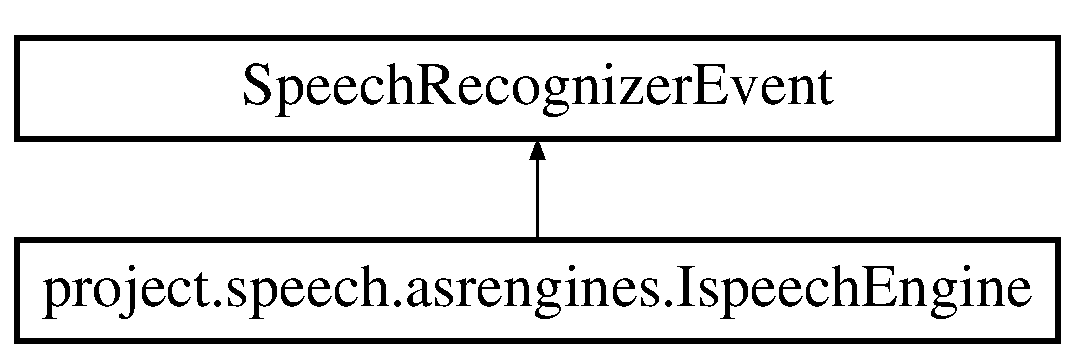
\includegraphics[height=2.000000cm]{classproject_1_1speech_1_1asrengines_1_1_ispeech_engine}
\end{center}
\end{figure}
\subsection*{Public Member Functions}
\begin{DoxyCompactItemize}
\item 
{\bf Ispeech\+Engine} ()
\item 
void {\bf run\+File} (File current\+Speech\+Folder, File current\+Speech\+Files, File reference\+File)  throws Exception 
\item 
void {\bf state\+Changed} (int event, int free\+Form\+Value, Exception last\+Exception)
\end{DoxyCompactItemize}
\subsection*{Private Attributes}
\begin{DoxyCompactItemize}
\item 
Array\+List$<$ String $>$ {\bf output\+Sentences\+Ispeech\+List} = new Array\+List$<$String$>$()
\item 
Array\+List$<$ String $>$ {\bf output\+File\+Names\+Ispeech\+List} = new Array\+List$<$String$>$()
\item 
double {\bf start\+Time\+Ms\+Ispeech}
\item 
double {\bf stop\+Time\+Ms\+Ispeech}
\item 
double {\bf time\+Diff\+Ispeech}
\end{DoxyCompactItemize}
\subsection*{Static Private Attributes}
\begin{DoxyCompactItemize}
\item 
static String {\bf api}
\item 
static boolean {\bf production}
\end{DoxyCompactItemize}


\subsection{Constructor \& Destructor Documentation}
\index{project\+::speech\+::asrengines\+::\+Ispeech\+Engine@{project\+::speech\+::asrengines\+::\+Ispeech\+Engine}!Ispeech\+Engine@{Ispeech\+Engine}}
\index{Ispeech\+Engine@{Ispeech\+Engine}!project\+::speech\+::asrengines\+::\+Ispeech\+Engine@{project\+::speech\+::asrengines\+::\+Ispeech\+Engine}}
\subsubsection[{Ispeech\+Engine}]{\setlength{\rightskip}{0pt plus 5cm}project.\+speech.\+asrengines.\+Ispeech\+Engine.\+Ispeech\+Engine (
\begin{DoxyParamCaption}
{}
\end{DoxyParamCaption}
)}\label{classproject_1_1speech_1_1asrengines_1_1_ispeech_engine_a3df65783c30f2a6af6f1702ed4541d4f}


\subsection{Member Function Documentation}
\index{project\+::speech\+::asrengines\+::\+Ispeech\+Engine@{project\+::speech\+::asrengines\+::\+Ispeech\+Engine}!run\+File@{run\+File}}
\index{run\+File@{run\+File}!project\+::speech\+::asrengines\+::\+Ispeech\+Engine@{project\+::speech\+::asrengines\+::\+Ispeech\+Engine}}
\subsubsection[{run\+File}]{\setlength{\rightskip}{0pt plus 5cm}void project.\+speech.\+asrengines.\+Ispeech\+Engine.\+run\+File (
\begin{DoxyParamCaption}
\item[{File}]{current\+Speech\+Folder, }
\item[{File}]{current\+Speech\+Files, }
\item[{File}]{reference\+File}
\end{DoxyParamCaption}
) throws Exception}\label{classproject_1_1speech_1_1asrengines_1_1_ispeech_engine_ae8d11abffca81068fe6f0e320c850a32}
\index{project\+::speech\+::asrengines\+::\+Ispeech\+Engine@{project\+::speech\+::asrengines\+::\+Ispeech\+Engine}!state\+Changed@{state\+Changed}}
\index{state\+Changed@{state\+Changed}!project\+::speech\+::asrengines\+::\+Ispeech\+Engine@{project\+::speech\+::asrengines\+::\+Ispeech\+Engine}}
\subsubsection[{state\+Changed}]{\setlength{\rightskip}{0pt plus 5cm}void project.\+speech.\+asrengines.\+Ispeech\+Engine.\+state\+Changed (
\begin{DoxyParamCaption}
\item[{int}]{event, }
\item[{int}]{free\+Form\+Value, }
\item[{Exception}]{last\+Exception}
\end{DoxyParamCaption}
)}\label{classproject_1_1speech_1_1asrengines_1_1_ispeech_engine_ad998ce02c0960c2f8a87483e8a4ecf6f}


\subsection{Member Data Documentation}
\index{project\+::speech\+::asrengines\+::\+Ispeech\+Engine@{project\+::speech\+::asrengines\+::\+Ispeech\+Engine}!api@{api}}
\index{api@{api}!project\+::speech\+::asrengines\+::\+Ispeech\+Engine@{project\+::speech\+::asrengines\+::\+Ispeech\+Engine}}
\subsubsection[{api}]{\setlength{\rightskip}{0pt plus 5cm}String project.\+speech.\+asrengines.\+Ispeech\+Engine.\+api\hspace{0.3cm}{\ttfamily [static]}, {\ttfamily [private]}}\label{classproject_1_1speech_1_1asrengines_1_1_ispeech_engine_a96d59d9b47d63be631354fd2773c1910}
\index{project\+::speech\+::asrengines\+::\+Ispeech\+Engine@{project\+::speech\+::asrengines\+::\+Ispeech\+Engine}!output\+File\+Names\+Ispeech\+List@{output\+File\+Names\+Ispeech\+List}}
\index{output\+File\+Names\+Ispeech\+List@{output\+File\+Names\+Ispeech\+List}!project\+::speech\+::asrengines\+::\+Ispeech\+Engine@{project\+::speech\+::asrengines\+::\+Ispeech\+Engine}}
\subsubsection[{output\+File\+Names\+Ispeech\+List}]{\setlength{\rightskip}{0pt plus 5cm}Array\+List$<$String$>$ project.\+speech.\+asrengines.\+Ispeech\+Engine.\+output\+File\+Names\+Ispeech\+List = new Array\+List$<$String$>$()\hspace{0.3cm}{\ttfamily [private]}}\label{classproject_1_1speech_1_1asrengines_1_1_ispeech_engine_a4d29e66408937ac4188229b4b2198132}
\index{project\+::speech\+::asrengines\+::\+Ispeech\+Engine@{project\+::speech\+::asrengines\+::\+Ispeech\+Engine}!output\+Sentences\+Ispeech\+List@{output\+Sentences\+Ispeech\+List}}
\index{output\+Sentences\+Ispeech\+List@{output\+Sentences\+Ispeech\+List}!project\+::speech\+::asrengines\+::\+Ispeech\+Engine@{project\+::speech\+::asrengines\+::\+Ispeech\+Engine}}
\subsubsection[{output\+Sentences\+Ispeech\+List}]{\setlength{\rightskip}{0pt plus 5cm}Array\+List$<$String$>$ project.\+speech.\+asrengines.\+Ispeech\+Engine.\+output\+Sentences\+Ispeech\+List = new Array\+List$<$String$>$()\hspace{0.3cm}{\ttfamily [private]}}\label{classproject_1_1speech_1_1asrengines_1_1_ispeech_engine_a2f96e80a8d364fb76e8b98be1cb2342c}
\index{project\+::speech\+::asrengines\+::\+Ispeech\+Engine@{project\+::speech\+::asrengines\+::\+Ispeech\+Engine}!production@{production}}
\index{production@{production}!project\+::speech\+::asrengines\+::\+Ispeech\+Engine@{project\+::speech\+::asrengines\+::\+Ispeech\+Engine}}
\subsubsection[{production}]{\setlength{\rightskip}{0pt plus 5cm}boolean project.\+speech.\+asrengines.\+Ispeech\+Engine.\+production\hspace{0.3cm}{\ttfamily [static]}, {\ttfamily [private]}}\label{classproject_1_1speech_1_1asrengines_1_1_ispeech_engine_a9660f67cd28dd76af87fe81e86111f86}
\index{project\+::speech\+::asrengines\+::\+Ispeech\+Engine@{project\+::speech\+::asrengines\+::\+Ispeech\+Engine}!start\+Time\+Ms\+Ispeech@{start\+Time\+Ms\+Ispeech}}
\index{start\+Time\+Ms\+Ispeech@{start\+Time\+Ms\+Ispeech}!project\+::speech\+::asrengines\+::\+Ispeech\+Engine@{project\+::speech\+::asrengines\+::\+Ispeech\+Engine}}
\subsubsection[{start\+Time\+Ms\+Ispeech}]{\setlength{\rightskip}{0pt plus 5cm}double project.\+speech.\+asrengines.\+Ispeech\+Engine.\+start\+Time\+Ms\+Ispeech\hspace{0.3cm}{\ttfamily [private]}}\label{classproject_1_1speech_1_1asrengines_1_1_ispeech_engine_af35ab752f183de83b5ba56643028c065}
\index{project\+::speech\+::asrengines\+::\+Ispeech\+Engine@{project\+::speech\+::asrengines\+::\+Ispeech\+Engine}!stop\+Time\+Ms\+Ispeech@{stop\+Time\+Ms\+Ispeech}}
\index{stop\+Time\+Ms\+Ispeech@{stop\+Time\+Ms\+Ispeech}!project\+::speech\+::asrengines\+::\+Ispeech\+Engine@{project\+::speech\+::asrengines\+::\+Ispeech\+Engine}}
\subsubsection[{stop\+Time\+Ms\+Ispeech}]{\setlength{\rightskip}{0pt plus 5cm}double project.\+speech.\+asrengines.\+Ispeech\+Engine.\+stop\+Time\+Ms\+Ispeech\hspace{0.3cm}{\ttfamily [private]}}\label{classproject_1_1speech_1_1asrengines_1_1_ispeech_engine_a273e73123f75fdb60e6e8a96448aa686}
\index{project\+::speech\+::asrengines\+::\+Ispeech\+Engine@{project\+::speech\+::asrengines\+::\+Ispeech\+Engine}!time\+Diff\+Ispeech@{time\+Diff\+Ispeech}}
\index{time\+Diff\+Ispeech@{time\+Diff\+Ispeech}!project\+::speech\+::asrengines\+::\+Ispeech\+Engine@{project\+::speech\+::asrengines\+::\+Ispeech\+Engine}}
\subsubsection[{time\+Diff\+Ispeech}]{\setlength{\rightskip}{0pt plus 5cm}double project.\+speech.\+asrengines.\+Ispeech\+Engine.\+time\+Diff\+Ispeech\hspace{0.3cm}{\ttfamily [private]}}\label{classproject_1_1speech_1_1asrengines_1_1_ispeech_engine_a0d129ec33fbe333f3337ceeead4e6994}


The documentation for this class was generated from the following file\+:\begin{DoxyCompactItemize}
\item 
project/speech/asrengines/{\bf Ispeech\+Engine.\+java}\end{DoxyCompactItemize}

\section{project.\+speech.\+user\+Interface.\+Ui\+Asr\+Properties Class Reference}
\label{classproject_1_1speech_1_1user_interface_1_1_ui_asr_properties}\index{project.\+speech.\+user\+Interface.\+Ui\+Asr\+Properties@{project.\+speech.\+user\+Interface.\+Ui\+Asr\+Properties}}
\subsection*{Public Member Functions}
\begin{DoxyCompactItemize}
\item 
File {\bf get\+Ui\+Speech\+Corpus} ()
\item 
void {\bf set\+Ui\+Speech\+Corpus} (File {\bf ui\+Speech\+Corpus})
\item 
File {\bf get\+Ui\+Dictionary} ()
\item 
void {\bf set\+Ui\+Dictionary} (File {\bf ui\+Dictionary})
\item 
File {\bf get\+Ui\+Acoustic} ()
\item 
void {\bf set\+Ui\+Acoustic} (File {\bf ui\+Acoustic})
\item 
File {\bf get\+Ui\+Language} ()
\item 
void {\bf set\+Ui\+Language} (File {\bf ui\+Language})
\end{DoxyCompactItemize}
\subsection*{Private Attributes}
\begin{DoxyCompactItemize}
\item 
File {\bf ui\+Speech\+Corpus}
\item 
File {\bf ui\+Dictionary}
\item 
File {\bf ui\+Acoustic}
\item 
File {\bf ui\+Language}
\end{DoxyCompactItemize}


\subsection{Member Function Documentation}
\index{project\+::speech\+::user\+Interface\+::\+Ui\+Asr\+Properties@{project\+::speech\+::user\+Interface\+::\+Ui\+Asr\+Properties}!get\+Ui\+Acoustic@{get\+Ui\+Acoustic}}
\index{get\+Ui\+Acoustic@{get\+Ui\+Acoustic}!project\+::speech\+::user\+Interface\+::\+Ui\+Asr\+Properties@{project\+::speech\+::user\+Interface\+::\+Ui\+Asr\+Properties}}
\subsubsection[{get\+Ui\+Acoustic}]{\setlength{\rightskip}{0pt plus 5cm}File project.\+speech.\+user\+Interface.\+Ui\+Asr\+Properties.\+get\+Ui\+Acoustic (
\begin{DoxyParamCaption}
{}
\end{DoxyParamCaption}
)}\label{classproject_1_1speech_1_1user_interface_1_1_ui_asr_properties_a0a24d501db131d911009a5e16d153e59}
Returns acoustic model path \begin{DoxyReturn}{Returns}
File path of acoustic file 
\end{DoxyReturn}
\index{project\+::speech\+::user\+Interface\+::\+Ui\+Asr\+Properties@{project\+::speech\+::user\+Interface\+::\+Ui\+Asr\+Properties}!get\+Ui\+Dictionary@{get\+Ui\+Dictionary}}
\index{get\+Ui\+Dictionary@{get\+Ui\+Dictionary}!project\+::speech\+::user\+Interface\+::\+Ui\+Asr\+Properties@{project\+::speech\+::user\+Interface\+::\+Ui\+Asr\+Properties}}
\subsubsection[{get\+Ui\+Dictionary}]{\setlength{\rightskip}{0pt plus 5cm}File project.\+speech.\+user\+Interface.\+Ui\+Asr\+Properties.\+get\+Ui\+Dictionary (
\begin{DoxyParamCaption}
{}
\end{DoxyParamCaption}
)}\label{classproject_1_1speech_1_1user_interface_1_1_ui_asr_properties_ae729b7ad4cfcd50e818eb9498e6c406e}
Returns dictionary model path \begin{DoxyReturn}{Returns}
File path of dictionary file 
\end{DoxyReturn}
\index{project\+::speech\+::user\+Interface\+::\+Ui\+Asr\+Properties@{project\+::speech\+::user\+Interface\+::\+Ui\+Asr\+Properties}!get\+Ui\+Language@{get\+Ui\+Language}}
\index{get\+Ui\+Language@{get\+Ui\+Language}!project\+::speech\+::user\+Interface\+::\+Ui\+Asr\+Properties@{project\+::speech\+::user\+Interface\+::\+Ui\+Asr\+Properties}}
\subsubsection[{get\+Ui\+Language}]{\setlength{\rightskip}{0pt plus 5cm}File project.\+speech.\+user\+Interface.\+Ui\+Asr\+Properties.\+get\+Ui\+Language (
\begin{DoxyParamCaption}
{}
\end{DoxyParamCaption}
)}\label{classproject_1_1speech_1_1user_interface_1_1_ui_asr_properties_a0291c402d178031aadab91eb5033c8d1}
Returns Language model path \begin{DoxyReturn}{Returns}
File path of language file 
\end{DoxyReturn}
\index{project\+::speech\+::user\+Interface\+::\+Ui\+Asr\+Properties@{project\+::speech\+::user\+Interface\+::\+Ui\+Asr\+Properties}!get\+Ui\+Speech\+Corpus@{get\+Ui\+Speech\+Corpus}}
\index{get\+Ui\+Speech\+Corpus@{get\+Ui\+Speech\+Corpus}!project\+::speech\+::user\+Interface\+::\+Ui\+Asr\+Properties@{project\+::speech\+::user\+Interface\+::\+Ui\+Asr\+Properties}}
\subsubsection[{get\+Ui\+Speech\+Corpus}]{\setlength{\rightskip}{0pt plus 5cm}File project.\+speech.\+user\+Interface.\+Ui\+Asr\+Properties.\+get\+Ui\+Speech\+Corpus (
\begin{DoxyParamCaption}
{}
\end{DoxyParamCaption}
)}\label{classproject_1_1speech_1_1user_interface_1_1_ui_asr_properties_a761950dc3c1892a7b388c6c505a23769}
Returns speech database path \begin{DoxyReturn}{Returns}
Folder path of the speech database 
\end{DoxyReturn}
\index{project\+::speech\+::user\+Interface\+::\+Ui\+Asr\+Properties@{project\+::speech\+::user\+Interface\+::\+Ui\+Asr\+Properties}!set\+Ui\+Acoustic@{set\+Ui\+Acoustic}}
\index{set\+Ui\+Acoustic@{set\+Ui\+Acoustic}!project\+::speech\+::user\+Interface\+::\+Ui\+Asr\+Properties@{project\+::speech\+::user\+Interface\+::\+Ui\+Asr\+Properties}}
\subsubsection[{set\+Ui\+Acoustic}]{\setlength{\rightskip}{0pt plus 5cm}void project.\+speech.\+user\+Interface.\+Ui\+Asr\+Properties.\+set\+Ui\+Acoustic (
\begin{DoxyParamCaption}
\item[{File}]{ui\+Acoustic}
\end{DoxyParamCaption}
)}\label{classproject_1_1speech_1_1user_interface_1_1_ui_asr_properties_ab2bb11978f492dd86eacc5689887cc08}
Sets acoustic file path 
\begin{DoxyParams}{Parameters}
{\em ui\+Acoustic} & File path of acoustic file \\
\hline
\end{DoxyParams}
\index{project\+::speech\+::user\+Interface\+::\+Ui\+Asr\+Properties@{project\+::speech\+::user\+Interface\+::\+Ui\+Asr\+Properties}!set\+Ui\+Dictionary@{set\+Ui\+Dictionary}}
\index{set\+Ui\+Dictionary@{set\+Ui\+Dictionary}!project\+::speech\+::user\+Interface\+::\+Ui\+Asr\+Properties@{project\+::speech\+::user\+Interface\+::\+Ui\+Asr\+Properties}}
\subsubsection[{set\+Ui\+Dictionary}]{\setlength{\rightskip}{0pt plus 5cm}void project.\+speech.\+user\+Interface.\+Ui\+Asr\+Properties.\+set\+Ui\+Dictionary (
\begin{DoxyParamCaption}
\item[{File}]{ui\+Dictionary}
\end{DoxyParamCaption}
)}\label{classproject_1_1speech_1_1user_interface_1_1_ui_asr_properties_abb8b36aa4bf54f677b3a50ca14ef377a}
Sets dictionary model path 
\begin{DoxyParams}{Parameters}
{\em ui\+Dictionary} & File path of dictionary file \\
\hline
\end{DoxyParams}
\index{project\+::speech\+::user\+Interface\+::\+Ui\+Asr\+Properties@{project\+::speech\+::user\+Interface\+::\+Ui\+Asr\+Properties}!set\+Ui\+Language@{set\+Ui\+Language}}
\index{set\+Ui\+Language@{set\+Ui\+Language}!project\+::speech\+::user\+Interface\+::\+Ui\+Asr\+Properties@{project\+::speech\+::user\+Interface\+::\+Ui\+Asr\+Properties}}
\subsubsection[{set\+Ui\+Language}]{\setlength{\rightskip}{0pt plus 5cm}void project.\+speech.\+user\+Interface.\+Ui\+Asr\+Properties.\+set\+Ui\+Language (
\begin{DoxyParamCaption}
\item[{File}]{ui\+Language}
\end{DoxyParamCaption}
)}\label{classproject_1_1speech_1_1user_interface_1_1_ui_asr_properties_a0c62495f17869c0c91b9008fb716000e}
Sets language file path 
\begin{DoxyParams}{Parameters}
{\em ui\+Language} & File path of language file \\
\hline
\end{DoxyParams}
\index{project\+::speech\+::user\+Interface\+::\+Ui\+Asr\+Properties@{project\+::speech\+::user\+Interface\+::\+Ui\+Asr\+Properties}!set\+Ui\+Speech\+Corpus@{set\+Ui\+Speech\+Corpus}}
\index{set\+Ui\+Speech\+Corpus@{set\+Ui\+Speech\+Corpus}!project\+::speech\+::user\+Interface\+::\+Ui\+Asr\+Properties@{project\+::speech\+::user\+Interface\+::\+Ui\+Asr\+Properties}}
\subsubsection[{set\+Ui\+Speech\+Corpus}]{\setlength{\rightskip}{0pt plus 5cm}void project.\+speech.\+user\+Interface.\+Ui\+Asr\+Properties.\+set\+Ui\+Speech\+Corpus (
\begin{DoxyParamCaption}
\item[{File}]{ui\+Speech\+Corpus}
\end{DoxyParamCaption}
)}\label{classproject_1_1speech_1_1user_interface_1_1_ui_asr_properties_a181d982d4bc101a80b499627d28190dd}
Sets speech database path 
\begin{DoxyParams}{Parameters}
{\em ui\+Speech\+Corpus} & Folder path of the speech database \\
\hline
\end{DoxyParams}


\subsection{Member Data Documentation}
\index{project\+::speech\+::user\+Interface\+::\+Ui\+Asr\+Properties@{project\+::speech\+::user\+Interface\+::\+Ui\+Asr\+Properties}!ui\+Acoustic@{ui\+Acoustic}}
\index{ui\+Acoustic@{ui\+Acoustic}!project\+::speech\+::user\+Interface\+::\+Ui\+Asr\+Properties@{project\+::speech\+::user\+Interface\+::\+Ui\+Asr\+Properties}}
\subsubsection[{ui\+Acoustic}]{\setlength{\rightskip}{0pt plus 5cm}File project.\+speech.\+user\+Interface.\+Ui\+Asr\+Properties.\+ui\+Acoustic\hspace{0.3cm}{\ttfamily [private]}}\label{classproject_1_1speech_1_1user_interface_1_1_ui_asr_properties_a8176c79b33ad3f2be82ff18b77751077}
\index{project\+::speech\+::user\+Interface\+::\+Ui\+Asr\+Properties@{project\+::speech\+::user\+Interface\+::\+Ui\+Asr\+Properties}!ui\+Dictionary@{ui\+Dictionary}}
\index{ui\+Dictionary@{ui\+Dictionary}!project\+::speech\+::user\+Interface\+::\+Ui\+Asr\+Properties@{project\+::speech\+::user\+Interface\+::\+Ui\+Asr\+Properties}}
\subsubsection[{ui\+Dictionary}]{\setlength{\rightskip}{0pt plus 5cm}File project.\+speech.\+user\+Interface.\+Ui\+Asr\+Properties.\+ui\+Dictionary\hspace{0.3cm}{\ttfamily [private]}}\label{classproject_1_1speech_1_1user_interface_1_1_ui_asr_properties_a145d6c60adf65497a8ee44cdecc76993}
\index{project\+::speech\+::user\+Interface\+::\+Ui\+Asr\+Properties@{project\+::speech\+::user\+Interface\+::\+Ui\+Asr\+Properties}!ui\+Language@{ui\+Language}}
\index{ui\+Language@{ui\+Language}!project\+::speech\+::user\+Interface\+::\+Ui\+Asr\+Properties@{project\+::speech\+::user\+Interface\+::\+Ui\+Asr\+Properties}}
\subsubsection[{ui\+Language}]{\setlength{\rightskip}{0pt plus 5cm}File project.\+speech.\+user\+Interface.\+Ui\+Asr\+Properties.\+ui\+Language\hspace{0.3cm}{\ttfamily [private]}}\label{classproject_1_1speech_1_1user_interface_1_1_ui_asr_properties_ad891b8ede2e34cc669acf75848720aa4}
\index{project\+::speech\+::user\+Interface\+::\+Ui\+Asr\+Properties@{project\+::speech\+::user\+Interface\+::\+Ui\+Asr\+Properties}!ui\+Speech\+Corpus@{ui\+Speech\+Corpus}}
\index{ui\+Speech\+Corpus@{ui\+Speech\+Corpus}!project\+::speech\+::user\+Interface\+::\+Ui\+Asr\+Properties@{project\+::speech\+::user\+Interface\+::\+Ui\+Asr\+Properties}}
\subsubsection[{ui\+Speech\+Corpus}]{\setlength{\rightskip}{0pt plus 5cm}File project.\+speech.\+user\+Interface.\+Ui\+Asr\+Properties.\+ui\+Speech\+Corpus\hspace{0.3cm}{\ttfamily [private]}}\label{classproject_1_1speech_1_1user_interface_1_1_ui_asr_properties_aa121a276dc88a5fe3e7b5edc4f1eea95}


The documentation for this class was generated from the following file\+:\begin{DoxyCompactItemize}
\item 
project/speech/user\+Interface/{\bf Ui\+Asr\+Properties.\+java}\end{DoxyCompactItemize}

\section{project.\+speech.\+user\+Interface.\+Ui\+Instruction\+Frame1 Class Reference}
\label{classproject_1_1speech_1_1user_interface_1_1_ui_instruction_frame1}\index{project.\+speech.\+user\+Interface.\+Ui\+Instruction\+Frame1@{project.\+speech.\+user\+Interface.\+Ui\+Instruction\+Frame1}}
Inheritance diagram for project.\+speech.\+user\+Interface.\+Ui\+Instruction\+Frame1\+:\begin{figure}[H]
\begin{center}
\leavevmode
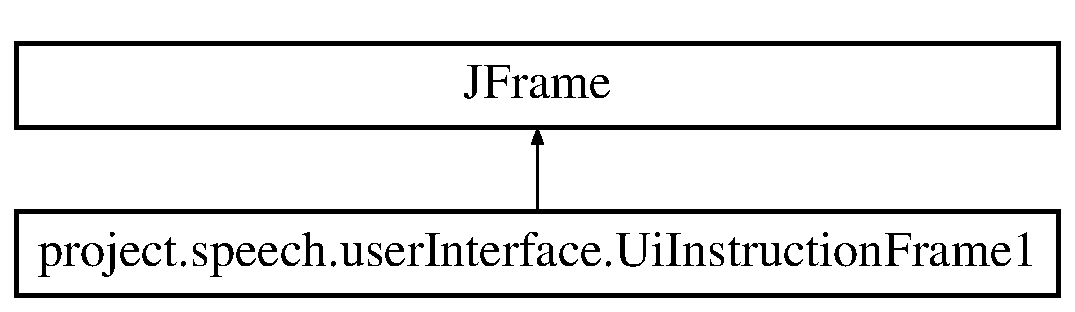
\includegraphics[height=2.000000cm]{classproject_1_1speech_1_1user_interface_1_1_ui_instruction_frame1}
\end{center}
\end{figure}
\subsection*{Public Member Functions}
\begin{DoxyCompactItemize}
\item 
{\bf Ui\+Instruction\+Frame1} ()
\end{DoxyCompactItemize}
\subsection*{Private Attributes}
\begin{DoxyCompactItemize}
\item 
J\+Panel {\bf content\+Pane}
\item 
J\+Panel {\bf panel\+Tree}
\item 
J\+Panel {\bf panel\+Steps}
\item 
J\+Label {\bf lbl\+Steps}
\item 
J\+Panel {\bf panel\+Note}
\item 
J\+Label {\bf lbl\+Note}
\item 
J\+Panel {\bf panel\+Transcript}
\item 
J\+Label {\bf lbl\+Transcript}
\item 
Buffered\+Image {\bf my\+Picture} = null
\item 
J\+Label {\bf lbl\+Performance2}
\end{DoxyCompactItemize}


\subsection{Constructor \& Destructor Documentation}
\index{project\+::speech\+::user\+Interface\+::\+Ui\+Instruction\+Frame1@{project\+::speech\+::user\+Interface\+::\+Ui\+Instruction\+Frame1}!Ui\+Instruction\+Frame1@{Ui\+Instruction\+Frame1}}
\index{Ui\+Instruction\+Frame1@{Ui\+Instruction\+Frame1}!project\+::speech\+::user\+Interface\+::\+Ui\+Instruction\+Frame1@{project\+::speech\+::user\+Interface\+::\+Ui\+Instruction\+Frame1}}
\subsubsection[{Ui\+Instruction\+Frame1}]{\setlength{\rightskip}{0pt plus 5cm}project.\+speech.\+user\+Interface.\+Ui\+Instruction\+Frame1.\+Ui\+Instruction\+Frame1 (
\begin{DoxyParamCaption}
{}
\end{DoxyParamCaption}
)}\label{classproject_1_1speech_1_1user_interface_1_1_ui_instruction_frame1_af8e5357bcc681ae396b5f25129f22754}


\subsection{Member Data Documentation}
\index{project\+::speech\+::user\+Interface\+::\+Ui\+Instruction\+Frame1@{project\+::speech\+::user\+Interface\+::\+Ui\+Instruction\+Frame1}!content\+Pane@{content\+Pane}}
\index{content\+Pane@{content\+Pane}!project\+::speech\+::user\+Interface\+::\+Ui\+Instruction\+Frame1@{project\+::speech\+::user\+Interface\+::\+Ui\+Instruction\+Frame1}}
\subsubsection[{content\+Pane}]{\setlength{\rightskip}{0pt plus 5cm}J\+Panel project.\+speech.\+user\+Interface.\+Ui\+Instruction\+Frame1.\+content\+Pane\hspace{0.3cm}{\ttfamily [private]}}\label{classproject_1_1speech_1_1user_interface_1_1_ui_instruction_frame1_a1654fbba46cb16f9cc1a3e4cf6d1ec87}
\index{project\+::speech\+::user\+Interface\+::\+Ui\+Instruction\+Frame1@{project\+::speech\+::user\+Interface\+::\+Ui\+Instruction\+Frame1}!lbl\+Note@{lbl\+Note}}
\index{lbl\+Note@{lbl\+Note}!project\+::speech\+::user\+Interface\+::\+Ui\+Instruction\+Frame1@{project\+::speech\+::user\+Interface\+::\+Ui\+Instruction\+Frame1}}
\subsubsection[{lbl\+Note}]{\setlength{\rightskip}{0pt plus 5cm}J\+Label project.\+speech.\+user\+Interface.\+Ui\+Instruction\+Frame1.\+lbl\+Note\hspace{0.3cm}{\ttfamily [private]}}\label{classproject_1_1speech_1_1user_interface_1_1_ui_instruction_frame1_a7175e51ce513679cdf0bbbd9c7ccbe69}
\index{project\+::speech\+::user\+Interface\+::\+Ui\+Instruction\+Frame1@{project\+::speech\+::user\+Interface\+::\+Ui\+Instruction\+Frame1}!lbl\+Performance2@{lbl\+Performance2}}
\index{lbl\+Performance2@{lbl\+Performance2}!project\+::speech\+::user\+Interface\+::\+Ui\+Instruction\+Frame1@{project\+::speech\+::user\+Interface\+::\+Ui\+Instruction\+Frame1}}
\subsubsection[{lbl\+Performance2}]{\setlength{\rightskip}{0pt plus 5cm}J\+Label project.\+speech.\+user\+Interface.\+Ui\+Instruction\+Frame1.\+lbl\+Performance2\hspace{0.3cm}{\ttfamily [private]}}\label{classproject_1_1speech_1_1user_interface_1_1_ui_instruction_frame1_aef2e7241dd78123ce1db98d294b05698}
\index{project\+::speech\+::user\+Interface\+::\+Ui\+Instruction\+Frame1@{project\+::speech\+::user\+Interface\+::\+Ui\+Instruction\+Frame1}!lbl\+Steps@{lbl\+Steps}}
\index{lbl\+Steps@{lbl\+Steps}!project\+::speech\+::user\+Interface\+::\+Ui\+Instruction\+Frame1@{project\+::speech\+::user\+Interface\+::\+Ui\+Instruction\+Frame1}}
\subsubsection[{lbl\+Steps}]{\setlength{\rightskip}{0pt plus 5cm}J\+Label project.\+speech.\+user\+Interface.\+Ui\+Instruction\+Frame1.\+lbl\+Steps\hspace{0.3cm}{\ttfamily [private]}}\label{classproject_1_1speech_1_1user_interface_1_1_ui_instruction_frame1_a133b30793a9d47ce7fdea4ee6e5240e1}
\index{project\+::speech\+::user\+Interface\+::\+Ui\+Instruction\+Frame1@{project\+::speech\+::user\+Interface\+::\+Ui\+Instruction\+Frame1}!lbl\+Transcript@{lbl\+Transcript}}
\index{lbl\+Transcript@{lbl\+Transcript}!project\+::speech\+::user\+Interface\+::\+Ui\+Instruction\+Frame1@{project\+::speech\+::user\+Interface\+::\+Ui\+Instruction\+Frame1}}
\subsubsection[{lbl\+Transcript}]{\setlength{\rightskip}{0pt plus 5cm}J\+Label project.\+speech.\+user\+Interface.\+Ui\+Instruction\+Frame1.\+lbl\+Transcript\hspace{0.3cm}{\ttfamily [private]}}\label{classproject_1_1speech_1_1user_interface_1_1_ui_instruction_frame1_ab2d1cec5942e170a47eb2466a629e499}
\index{project\+::speech\+::user\+Interface\+::\+Ui\+Instruction\+Frame1@{project\+::speech\+::user\+Interface\+::\+Ui\+Instruction\+Frame1}!my\+Picture@{my\+Picture}}
\index{my\+Picture@{my\+Picture}!project\+::speech\+::user\+Interface\+::\+Ui\+Instruction\+Frame1@{project\+::speech\+::user\+Interface\+::\+Ui\+Instruction\+Frame1}}
\subsubsection[{my\+Picture}]{\setlength{\rightskip}{0pt plus 5cm}Buffered\+Image project.\+speech.\+user\+Interface.\+Ui\+Instruction\+Frame1.\+my\+Picture = null\hspace{0.3cm}{\ttfamily [private]}}\label{classproject_1_1speech_1_1user_interface_1_1_ui_instruction_frame1_aa51a880230d7a86734d02921a0b81c4b}
\index{project\+::speech\+::user\+Interface\+::\+Ui\+Instruction\+Frame1@{project\+::speech\+::user\+Interface\+::\+Ui\+Instruction\+Frame1}!panel\+Note@{panel\+Note}}
\index{panel\+Note@{panel\+Note}!project\+::speech\+::user\+Interface\+::\+Ui\+Instruction\+Frame1@{project\+::speech\+::user\+Interface\+::\+Ui\+Instruction\+Frame1}}
\subsubsection[{panel\+Note}]{\setlength{\rightskip}{0pt plus 5cm}J\+Panel project.\+speech.\+user\+Interface.\+Ui\+Instruction\+Frame1.\+panel\+Note\hspace{0.3cm}{\ttfamily [private]}}\label{classproject_1_1speech_1_1user_interface_1_1_ui_instruction_frame1_a7498f2257480d84170eb65c322ff7c85}
\index{project\+::speech\+::user\+Interface\+::\+Ui\+Instruction\+Frame1@{project\+::speech\+::user\+Interface\+::\+Ui\+Instruction\+Frame1}!panel\+Steps@{panel\+Steps}}
\index{panel\+Steps@{panel\+Steps}!project\+::speech\+::user\+Interface\+::\+Ui\+Instruction\+Frame1@{project\+::speech\+::user\+Interface\+::\+Ui\+Instruction\+Frame1}}
\subsubsection[{panel\+Steps}]{\setlength{\rightskip}{0pt plus 5cm}J\+Panel project.\+speech.\+user\+Interface.\+Ui\+Instruction\+Frame1.\+panel\+Steps\hspace{0.3cm}{\ttfamily [private]}}\label{classproject_1_1speech_1_1user_interface_1_1_ui_instruction_frame1_ace71335faaddb330f819281e82df7c11}
\index{project\+::speech\+::user\+Interface\+::\+Ui\+Instruction\+Frame1@{project\+::speech\+::user\+Interface\+::\+Ui\+Instruction\+Frame1}!panel\+Transcript@{panel\+Transcript}}
\index{panel\+Transcript@{panel\+Transcript}!project\+::speech\+::user\+Interface\+::\+Ui\+Instruction\+Frame1@{project\+::speech\+::user\+Interface\+::\+Ui\+Instruction\+Frame1}}
\subsubsection[{panel\+Transcript}]{\setlength{\rightskip}{0pt plus 5cm}J\+Panel project.\+speech.\+user\+Interface.\+Ui\+Instruction\+Frame1.\+panel\+Transcript\hspace{0.3cm}{\ttfamily [private]}}\label{classproject_1_1speech_1_1user_interface_1_1_ui_instruction_frame1_a8c31fcef9e437645eaf15d714368f00d}
\index{project\+::speech\+::user\+Interface\+::\+Ui\+Instruction\+Frame1@{project\+::speech\+::user\+Interface\+::\+Ui\+Instruction\+Frame1}!panel\+Tree@{panel\+Tree}}
\index{panel\+Tree@{panel\+Tree}!project\+::speech\+::user\+Interface\+::\+Ui\+Instruction\+Frame1@{project\+::speech\+::user\+Interface\+::\+Ui\+Instruction\+Frame1}}
\subsubsection[{panel\+Tree}]{\setlength{\rightskip}{0pt plus 5cm}J\+Panel project.\+speech.\+user\+Interface.\+Ui\+Instruction\+Frame1.\+panel\+Tree\hspace{0.3cm}{\ttfamily [private]}}\label{classproject_1_1speech_1_1user_interface_1_1_ui_instruction_frame1_a602ed08e80d737c5d95412b4f2cb311e}


The documentation for this class was generated from the following file\+:\begin{DoxyCompactItemize}
\item 
project/speech/user\+Interface/{\bf Ui\+Instruction\+Frame1.\+java}\end{DoxyCompactItemize}

\section{project.\+speech.\+user\+Interface.\+Ui\+Instruction\+Frame2 Class Reference}
\label{classproject_1_1speech_1_1user_interface_1_1_ui_instruction_frame2}\index{project.\+speech.\+user\+Interface.\+Ui\+Instruction\+Frame2@{project.\+speech.\+user\+Interface.\+Ui\+Instruction\+Frame2}}
Inheritance diagram for project.\+speech.\+user\+Interface.\+Ui\+Instruction\+Frame2\+:\begin{figure}[H]
\begin{center}
\leavevmode
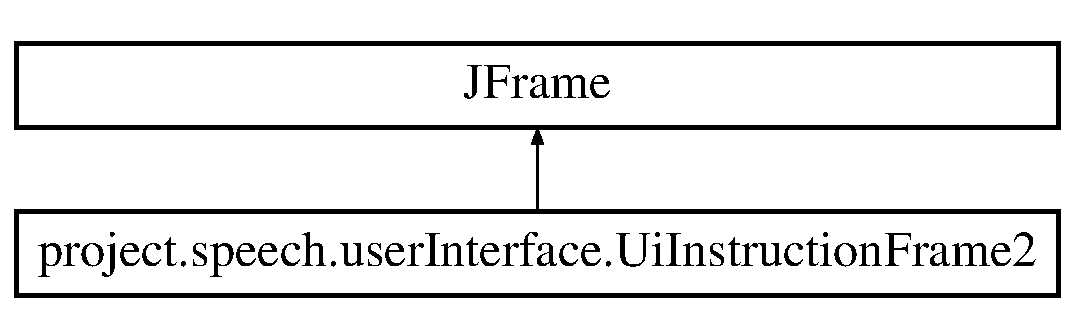
\includegraphics[height=2.000000cm]{classproject_1_1speech_1_1user_interface_1_1_ui_instruction_frame2}
\end{center}
\end{figure}
\subsection*{Public Member Functions}
\begin{DoxyCompactItemize}
\item 
{\bf Ui\+Instruction\+Frame2} ()
\end{DoxyCompactItemize}
\subsection*{Private Attributes}
\begin{DoxyCompactItemize}
\item 
J\+Panel {\bf content\+Pane}
\item 
J\+Panel {\bf panel\+Instructions}
\item 
J\+Label {\bf lbl\+Steps}
\item 
J\+Panel {\bf panel\+Transcript}
\item 
J\+Label {\bf lbl\+Transcript}
\item 
J\+Panel {\bf panel}
\item 
J\+Label {\bf label}
\item 
J\+Label {\bf lblwer\+Word}
\end{DoxyCompactItemize}


\subsection{Constructor \& Destructor Documentation}
\index{project\+::speech\+::user\+Interface\+::\+Ui\+Instruction\+Frame2@{project\+::speech\+::user\+Interface\+::\+Ui\+Instruction\+Frame2}!Ui\+Instruction\+Frame2@{Ui\+Instruction\+Frame2}}
\index{Ui\+Instruction\+Frame2@{Ui\+Instruction\+Frame2}!project\+::speech\+::user\+Interface\+::\+Ui\+Instruction\+Frame2@{project\+::speech\+::user\+Interface\+::\+Ui\+Instruction\+Frame2}}
\subsubsection[{Ui\+Instruction\+Frame2}]{\setlength{\rightskip}{0pt plus 5cm}project.\+speech.\+user\+Interface.\+Ui\+Instruction\+Frame2.\+Ui\+Instruction\+Frame2 (
\begin{DoxyParamCaption}
{}
\end{DoxyParamCaption}
)}\label{classproject_1_1speech_1_1user_interface_1_1_ui_instruction_frame2_a410d29474a94593eb94111fa1992b217}


\subsection{Member Data Documentation}
\index{project\+::speech\+::user\+Interface\+::\+Ui\+Instruction\+Frame2@{project\+::speech\+::user\+Interface\+::\+Ui\+Instruction\+Frame2}!content\+Pane@{content\+Pane}}
\index{content\+Pane@{content\+Pane}!project\+::speech\+::user\+Interface\+::\+Ui\+Instruction\+Frame2@{project\+::speech\+::user\+Interface\+::\+Ui\+Instruction\+Frame2}}
\subsubsection[{content\+Pane}]{\setlength{\rightskip}{0pt plus 5cm}J\+Panel project.\+speech.\+user\+Interface.\+Ui\+Instruction\+Frame2.\+content\+Pane\hspace{0.3cm}{\ttfamily [private]}}\label{classproject_1_1speech_1_1user_interface_1_1_ui_instruction_frame2_a8fbe72e15ebbb09291a74be8be87782b}
\index{project\+::speech\+::user\+Interface\+::\+Ui\+Instruction\+Frame2@{project\+::speech\+::user\+Interface\+::\+Ui\+Instruction\+Frame2}!label@{label}}
\index{label@{label}!project\+::speech\+::user\+Interface\+::\+Ui\+Instruction\+Frame2@{project\+::speech\+::user\+Interface\+::\+Ui\+Instruction\+Frame2}}
\subsubsection[{label}]{\setlength{\rightskip}{0pt plus 5cm}J\+Label project.\+speech.\+user\+Interface.\+Ui\+Instruction\+Frame2.\+label\hspace{0.3cm}{\ttfamily [private]}}\label{classproject_1_1speech_1_1user_interface_1_1_ui_instruction_frame2_abdcea3a58333e91a007e0798dc0e3610}
\index{project\+::speech\+::user\+Interface\+::\+Ui\+Instruction\+Frame2@{project\+::speech\+::user\+Interface\+::\+Ui\+Instruction\+Frame2}!lbl\+Steps@{lbl\+Steps}}
\index{lbl\+Steps@{lbl\+Steps}!project\+::speech\+::user\+Interface\+::\+Ui\+Instruction\+Frame2@{project\+::speech\+::user\+Interface\+::\+Ui\+Instruction\+Frame2}}
\subsubsection[{lbl\+Steps}]{\setlength{\rightskip}{0pt plus 5cm}J\+Label project.\+speech.\+user\+Interface.\+Ui\+Instruction\+Frame2.\+lbl\+Steps\hspace{0.3cm}{\ttfamily [private]}}\label{classproject_1_1speech_1_1user_interface_1_1_ui_instruction_frame2_acf55e44dd73788f9cf965b5336f01a80}
\index{project\+::speech\+::user\+Interface\+::\+Ui\+Instruction\+Frame2@{project\+::speech\+::user\+Interface\+::\+Ui\+Instruction\+Frame2}!lbl\+Transcript@{lbl\+Transcript}}
\index{lbl\+Transcript@{lbl\+Transcript}!project\+::speech\+::user\+Interface\+::\+Ui\+Instruction\+Frame2@{project\+::speech\+::user\+Interface\+::\+Ui\+Instruction\+Frame2}}
\subsubsection[{lbl\+Transcript}]{\setlength{\rightskip}{0pt plus 5cm}J\+Label project.\+speech.\+user\+Interface.\+Ui\+Instruction\+Frame2.\+lbl\+Transcript\hspace{0.3cm}{\ttfamily [private]}}\label{classproject_1_1speech_1_1user_interface_1_1_ui_instruction_frame2_a39e7aabd3d87b88fbd78ebb227a0918f}
\index{project\+::speech\+::user\+Interface\+::\+Ui\+Instruction\+Frame2@{project\+::speech\+::user\+Interface\+::\+Ui\+Instruction\+Frame2}!lblwer\+Word@{lblwer\+Word}}
\index{lblwer\+Word@{lblwer\+Word}!project\+::speech\+::user\+Interface\+::\+Ui\+Instruction\+Frame2@{project\+::speech\+::user\+Interface\+::\+Ui\+Instruction\+Frame2}}
\subsubsection[{lblwer\+Word}]{\setlength{\rightskip}{0pt plus 5cm}J\+Label project.\+speech.\+user\+Interface.\+Ui\+Instruction\+Frame2.\+lblwer\+Word\hspace{0.3cm}{\ttfamily [private]}}\label{classproject_1_1speech_1_1user_interface_1_1_ui_instruction_frame2_afc19912c4f107f62f7abe2be3ff6fbdd}
\index{project\+::speech\+::user\+Interface\+::\+Ui\+Instruction\+Frame2@{project\+::speech\+::user\+Interface\+::\+Ui\+Instruction\+Frame2}!panel@{panel}}
\index{panel@{panel}!project\+::speech\+::user\+Interface\+::\+Ui\+Instruction\+Frame2@{project\+::speech\+::user\+Interface\+::\+Ui\+Instruction\+Frame2}}
\subsubsection[{panel}]{\setlength{\rightskip}{0pt plus 5cm}J\+Panel project.\+speech.\+user\+Interface.\+Ui\+Instruction\+Frame2.\+panel\hspace{0.3cm}{\ttfamily [private]}}\label{classproject_1_1speech_1_1user_interface_1_1_ui_instruction_frame2_a4a3b7f293a13d8f01c7e2c69faad8fcc}
\index{project\+::speech\+::user\+Interface\+::\+Ui\+Instruction\+Frame2@{project\+::speech\+::user\+Interface\+::\+Ui\+Instruction\+Frame2}!panel\+Instructions@{panel\+Instructions}}
\index{panel\+Instructions@{panel\+Instructions}!project\+::speech\+::user\+Interface\+::\+Ui\+Instruction\+Frame2@{project\+::speech\+::user\+Interface\+::\+Ui\+Instruction\+Frame2}}
\subsubsection[{panel\+Instructions}]{\setlength{\rightskip}{0pt plus 5cm}J\+Panel project.\+speech.\+user\+Interface.\+Ui\+Instruction\+Frame2.\+panel\+Instructions\hspace{0.3cm}{\ttfamily [private]}}\label{classproject_1_1speech_1_1user_interface_1_1_ui_instruction_frame2_ac2544a6dde59201deb0321eba1a07470}
\index{project\+::speech\+::user\+Interface\+::\+Ui\+Instruction\+Frame2@{project\+::speech\+::user\+Interface\+::\+Ui\+Instruction\+Frame2}!panel\+Transcript@{panel\+Transcript}}
\index{panel\+Transcript@{panel\+Transcript}!project\+::speech\+::user\+Interface\+::\+Ui\+Instruction\+Frame2@{project\+::speech\+::user\+Interface\+::\+Ui\+Instruction\+Frame2}}
\subsubsection[{panel\+Transcript}]{\setlength{\rightskip}{0pt plus 5cm}J\+Panel project.\+speech.\+user\+Interface.\+Ui\+Instruction\+Frame2.\+panel\+Transcript\hspace{0.3cm}{\ttfamily [private]}}\label{classproject_1_1speech_1_1user_interface_1_1_ui_instruction_frame2_a2323bbb36d7b03268e82fbe45ef19e89}


The documentation for this class was generated from the following file\+:\begin{DoxyCompactItemize}
\item 
project/speech/user\+Interface/{\bf Ui\+Instruction\+Frame2.\+java}\end{DoxyCompactItemize}

\section{project.\+speech.\+user\+Interface.\+Ui\+Instruction\+Main\+Frame Class Reference}
\label{classproject_1_1speech_1_1user_interface_1_1_ui_instruction_main_frame}\index{project.\+speech.\+user\+Interface.\+Ui\+Instruction\+Main\+Frame@{project.\+speech.\+user\+Interface.\+Ui\+Instruction\+Main\+Frame}}
Inheritance diagram for project.\+speech.\+user\+Interface.\+Ui\+Instruction\+Main\+Frame\+:\begin{figure}[H]
\begin{center}
\leavevmode
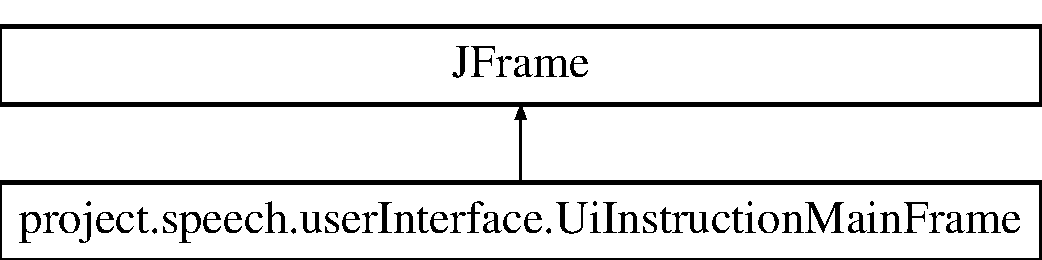
\includegraphics[height=2.000000cm]{classproject_1_1speech_1_1user_interface_1_1_ui_instruction_main_frame}
\end{center}
\end{figure}
\subsection*{Public Member Functions}
\begin{DoxyCompactItemize}
\item 
{\bf Ui\+Instruction\+Main\+Frame} ()
\end{DoxyCompactItemize}
\subsection*{Private Attributes}
\begin{DoxyCompactItemize}
\item 
J\+Panel {\bf content\+Pane}
\item 
J\+Panel {\bf panel\+Model1}
\item 
J\+Panel {\bf panel\+Model2}
\item 
J\+Label {\bf lbl\+Model1}
\item 
J\+Label {\bf lbl\+Model2}
\end{DoxyCompactItemize}


\subsection{Constructor \& Destructor Documentation}
\index{project\+::speech\+::user\+Interface\+::\+Ui\+Instruction\+Main\+Frame@{project\+::speech\+::user\+Interface\+::\+Ui\+Instruction\+Main\+Frame}!Ui\+Instruction\+Main\+Frame@{Ui\+Instruction\+Main\+Frame}}
\index{Ui\+Instruction\+Main\+Frame@{Ui\+Instruction\+Main\+Frame}!project\+::speech\+::user\+Interface\+::\+Ui\+Instruction\+Main\+Frame@{project\+::speech\+::user\+Interface\+::\+Ui\+Instruction\+Main\+Frame}}
\subsubsection[{Ui\+Instruction\+Main\+Frame}]{\setlength{\rightskip}{0pt plus 5cm}project.\+speech.\+user\+Interface.\+Ui\+Instruction\+Main\+Frame.\+Ui\+Instruction\+Main\+Frame (
\begin{DoxyParamCaption}
{}
\end{DoxyParamCaption}
)}\label{classproject_1_1speech_1_1user_interface_1_1_ui_instruction_main_frame_a649c7230bd99ac399db4edffbd17a9cd}


\subsection{Member Data Documentation}
\index{project\+::speech\+::user\+Interface\+::\+Ui\+Instruction\+Main\+Frame@{project\+::speech\+::user\+Interface\+::\+Ui\+Instruction\+Main\+Frame}!content\+Pane@{content\+Pane}}
\index{content\+Pane@{content\+Pane}!project\+::speech\+::user\+Interface\+::\+Ui\+Instruction\+Main\+Frame@{project\+::speech\+::user\+Interface\+::\+Ui\+Instruction\+Main\+Frame}}
\subsubsection[{content\+Pane}]{\setlength{\rightskip}{0pt plus 5cm}J\+Panel project.\+speech.\+user\+Interface.\+Ui\+Instruction\+Main\+Frame.\+content\+Pane\hspace{0.3cm}{\ttfamily [private]}}\label{classproject_1_1speech_1_1user_interface_1_1_ui_instruction_main_frame_ad8a9fffbac5ae79df9b58ce0bb58e044}
\index{project\+::speech\+::user\+Interface\+::\+Ui\+Instruction\+Main\+Frame@{project\+::speech\+::user\+Interface\+::\+Ui\+Instruction\+Main\+Frame}!lbl\+Model1@{lbl\+Model1}}
\index{lbl\+Model1@{lbl\+Model1}!project\+::speech\+::user\+Interface\+::\+Ui\+Instruction\+Main\+Frame@{project\+::speech\+::user\+Interface\+::\+Ui\+Instruction\+Main\+Frame}}
\subsubsection[{lbl\+Model1}]{\setlength{\rightskip}{0pt plus 5cm}J\+Label project.\+speech.\+user\+Interface.\+Ui\+Instruction\+Main\+Frame.\+lbl\+Model1\hspace{0.3cm}{\ttfamily [private]}}\label{classproject_1_1speech_1_1user_interface_1_1_ui_instruction_main_frame_a50f6b54e039035a1c4c5fa7b3d0c0515}
\index{project\+::speech\+::user\+Interface\+::\+Ui\+Instruction\+Main\+Frame@{project\+::speech\+::user\+Interface\+::\+Ui\+Instruction\+Main\+Frame}!lbl\+Model2@{lbl\+Model2}}
\index{lbl\+Model2@{lbl\+Model2}!project\+::speech\+::user\+Interface\+::\+Ui\+Instruction\+Main\+Frame@{project\+::speech\+::user\+Interface\+::\+Ui\+Instruction\+Main\+Frame}}
\subsubsection[{lbl\+Model2}]{\setlength{\rightskip}{0pt plus 5cm}J\+Label project.\+speech.\+user\+Interface.\+Ui\+Instruction\+Main\+Frame.\+lbl\+Model2\hspace{0.3cm}{\ttfamily [private]}}\label{classproject_1_1speech_1_1user_interface_1_1_ui_instruction_main_frame_a5277b931f0fef7e0fb78c573dc3290cf}
\index{project\+::speech\+::user\+Interface\+::\+Ui\+Instruction\+Main\+Frame@{project\+::speech\+::user\+Interface\+::\+Ui\+Instruction\+Main\+Frame}!panel\+Model1@{panel\+Model1}}
\index{panel\+Model1@{panel\+Model1}!project\+::speech\+::user\+Interface\+::\+Ui\+Instruction\+Main\+Frame@{project\+::speech\+::user\+Interface\+::\+Ui\+Instruction\+Main\+Frame}}
\subsubsection[{panel\+Model1}]{\setlength{\rightskip}{0pt plus 5cm}J\+Panel project.\+speech.\+user\+Interface.\+Ui\+Instruction\+Main\+Frame.\+panel\+Model1\hspace{0.3cm}{\ttfamily [private]}}\label{classproject_1_1speech_1_1user_interface_1_1_ui_instruction_main_frame_a1915c8243e411812a25c256fa3be5e00}
\index{project\+::speech\+::user\+Interface\+::\+Ui\+Instruction\+Main\+Frame@{project\+::speech\+::user\+Interface\+::\+Ui\+Instruction\+Main\+Frame}!panel\+Model2@{panel\+Model2}}
\index{panel\+Model2@{panel\+Model2}!project\+::speech\+::user\+Interface\+::\+Ui\+Instruction\+Main\+Frame@{project\+::speech\+::user\+Interface\+::\+Ui\+Instruction\+Main\+Frame}}
\subsubsection[{panel\+Model2}]{\setlength{\rightskip}{0pt plus 5cm}J\+Panel project.\+speech.\+user\+Interface.\+Ui\+Instruction\+Main\+Frame.\+panel\+Model2\hspace{0.3cm}{\ttfamily [private]}}\label{classproject_1_1speech_1_1user_interface_1_1_ui_instruction_main_frame_a543874daafc0fc6cad3f29745f5f94c9}


The documentation for this class was generated from the following file\+:\begin{DoxyCompactItemize}
\item 
project/speech/user\+Interface/{\bf Ui\+Instruction\+Main\+Frame.\+java}\end{DoxyCompactItemize}

\section{project.\+speech.\+user\+Interface.\+Ui\+Main\+Frame Class Reference}
\label{classproject_1_1speech_1_1user_interface_1_1_ui_main_frame}\index{project.\+speech.\+user\+Interface.\+Ui\+Main\+Frame@{project.\+speech.\+user\+Interface.\+Ui\+Main\+Frame}}
Inheritance diagram for project.\+speech.\+user\+Interface.\+Ui\+Main\+Frame\+:\begin{figure}[H]
\begin{center}
\leavevmode
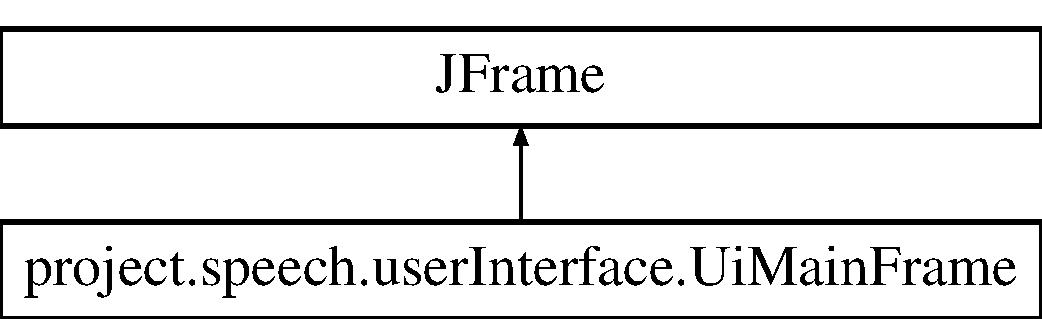
\includegraphics[height=2.000000cm]{classproject_1_1speech_1_1user_interface_1_1_ui_main_frame}
\end{center}
\end{figure}
\subsection*{Public Member Functions}
\begin{DoxyCompactItemize}
\item 
{\bf Ui\+Main\+Frame} ()
\end{DoxyCompactItemize}
\subsection*{Static Public Member Functions}
\begin{DoxyCompactItemize}
\item 
static void {\bf main} (String[$\,$] args)
\end{DoxyCompactItemize}
\subsection*{Static Private Attributes}
\begin{DoxyCompactItemize}
\item 
static final long {\bf serial\+Version\+U\+I\+D} = 1\+L
\item 
static J\+Panel {\bf content\+Pane}
\item 
static J\+Button {\bf btn\+Model1}
\item 
static J\+Button {\bf btn\+Model2}
\item 
static J\+Button {\bf btn\+Instructions}
\item 
static J\+Label {\bf lbl\+Asr\+Tool}
\end{DoxyCompactItemize}


\subsection{Constructor \& Destructor Documentation}
\index{project\+::speech\+::user\+Interface\+::\+Ui\+Main\+Frame@{project\+::speech\+::user\+Interface\+::\+Ui\+Main\+Frame}!Ui\+Main\+Frame@{Ui\+Main\+Frame}}
\index{Ui\+Main\+Frame@{Ui\+Main\+Frame}!project\+::speech\+::user\+Interface\+::\+Ui\+Main\+Frame@{project\+::speech\+::user\+Interface\+::\+Ui\+Main\+Frame}}
\subsubsection[{Ui\+Main\+Frame}]{\setlength{\rightskip}{0pt plus 5cm}project.\+speech.\+user\+Interface.\+Ui\+Main\+Frame.\+Ui\+Main\+Frame (
\begin{DoxyParamCaption}
{}
\end{DoxyParamCaption}
)}\label{classproject_1_1speech_1_1user_interface_1_1_ui_main_frame_aba01766b9fa5c3d4d745260f1a84b974}


\subsection{Member Function Documentation}
\index{project\+::speech\+::user\+Interface\+::\+Ui\+Main\+Frame@{project\+::speech\+::user\+Interface\+::\+Ui\+Main\+Frame}!main@{main}}
\index{main@{main}!project\+::speech\+::user\+Interface\+::\+Ui\+Main\+Frame@{project\+::speech\+::user\+Interface\+::\+Ui\+Main\+Frame}}
\subsubsection[{main}]{\setlength{\rightskip}{0pt plus 5cm}static void project.\+speech.\+user\+Interface.\+Ui\+Main\+Frame.\+main (
\begin{DoxyParamCaption}
\item[{String[$\,$]}]{args}
\end{DoxyParamCaption}
)\hspace{0.3cm}{\ttfamily [static]}}\label{classproject_1_1speech_1_1user_interface_1_1_ui_main_frame_adf9e24a550e0a34545a683fb36478e52}


\subsection{Member Data Documentation}
\index{project\+::speech\+::user\+Interface\+::\+Ui\+Main\+Frame@{project\+::speech\+::user\+Interface\+::\+Ui\+Main\+Frame}!btn\+Instructions@{btn\+Instructions}}
\index{btn\+Instructions@{btn\+Instructions}!project\+::speech\+::user\+Interface\+::\+Ui\+Main\+Frame@{project\+::speech\+::user\+Interface\+::\+Ui\+Main\+Frame}}
\subsubsection[{btn\+Instructions}]{\setlength{\rightskip}{0pt plus 5cm}J\+Button project.\+speech.\+user\+Interface.\+Ui\+Main\+Frame.\+btn\+Instructions\hspace{0.3cm}{\ttfamily [static]}, {\ttfamily [private]}}\label{classproject_1_1speech_1_1user_interface_1_1_ui_main_frame_aaab97a5abaf2c0c70f6a47029f3813f0}
\index{project\+::speech\+::user\+Interface\+::\+Ui\+Main\+Frame@{project\+::speech\+::user\+Interface\+::\+Ui\+Main\+Frame}!btn\+Model1@{btn\+Model1}}
\index{btn\+Model1@{btn\+Model1}!project\+::speech\+::user\+Interface\+::\+Ui\+Main\+Frame@{project\+::speech\+::user\+Interface\+::\+Ui\+Main\+Frame}}
\subsubsection[{btn\+Model1}]{\setlength{\rightskip}{0pt plus 5cm}J\+Button project.\+speech.\+user\+Interface.\+Ui\+Main\+Frame.\+btn\+Model1\hspace{0.3cm}{\ttfamily [static]}, {\ttfamily [private]}}\label{classproject_1_1speech_1_1user_interface_1_1_ui_main_frame_ab73cc6609c5cd32cce950f3d842bfe04}
\index{project\+::speech\+::user\+Interface\+::\+Ui\+Main\+Frame@{project\+::speech\+::user\+Interface\+::\+Ui\+Main\+Frame}!btn\+Model2@{btn\+Model2}}
\index{btn\+Model2@{btn\+Model2}!project\+::speech\+::user\+Interface\+::\+Ui\+Main\+Frame@{project\+::speech\+::user\+Interface\+::\+Ui\+Main\+Frame}}
\subsubsection[{btn\+Model2}]{\setlength{\rightskip}{0pt plus 5cm}J\+Button project.\+speech.\+user\+Interface.\+Ui\+Main\+Frame.\+btn\+Model2\hspace{0.3cm}{\ttfamily [static]}, {\ttfamily [private]}}\label{classproject_1_1speech_1_1user_interface_1_1_ui_main_frame_afaad6fbc5576e1d815d4f929ee5072b4}
\index{project\+::speech\+::user\+Interface\+::\+Ui\+Main\+Frame@{project\+::speech\+::user\+Interface\+::\+Ui\+Main\+Frame}!content\+Pane@{content\+Pane}}
\index{content\+Pane@{content\+Pane}!project\+::speech\+::user\+Interface\+::\+Ui\+Main\+Frame@{project\+::speech\+::user\+Interface\+::\+Ui\+Main\+Frame}}
\subsubsection[{content\+Pane}]{\setlength{\rightskip}{0pt plus 5cm}J\+Panel project.\+speech.\+user\+Interface.\+Ui\+Main\+Frame.\+content\+Pane\hspace{0.3cm}{\ttfamily [static]}, {\ttfamily [private]}}\label{classproject_1_1speech_1_1user_interface_1_1_ui_main_frame_a5bc09ca52031f4c875e2037d7bd8fea6}
\index{project\+::speech\+::user\+Interface\+::\+Ui\+Main\+Frame@{project\+::speech\+::user\+Interface\+::\+Ui\+Main\+Frame}!lbl\+Asr\+Tool@{lbl\+Asr\+Tool}}
\index{lbl\+Asr\+Tool@{lbl\+Asr\+Tool}!project\+::speech\+::user\+Interface\+::\+Ui\+Main\+Frame@{project\+::speech\+::user\+Interface\+::\+Ui\+Main\+Frame}}
\subsubsection[{lbl\+Asr\+Tool}]{\setlength{\rightskip}{0pt plus 5cm}J\+Label project.\+speech.\+user\+Interface.\+Ui\+Main\+Frame.\+lbl\+Asr\+Tool\hspace{0.3cm}{\ttfamily [static]}, {\ttfamily [private]}}\label{classproject_1_1speech_1_1user_interface_1_1_ui_main_frame_a582d52a29f63166c169a8dc8796d52ed}
\index{project\+::speech\+::user\+Interface\+::\+Ui\+Main\+Frame@{project\+::speech\+::user\+Interface\+::\+Ui\+Main\+Frame}!serial\+Version\+U\+I\+D@{serial\+Version\+U\+I\+D}}
\index{serial\+Version\+U\+I\+D@{serial\+Version\+U\+I\+D}!project\+::speech\+::user\+Interface\+::\+Ui\+Main\+Frame@{project\+::speech\+::user\+Interface\+::\+Ui\+Main\+Frame}}
\subsubsection[{serial\+Version\+U\+I\+D}]{\setlength{\rightskip}{0pt plus 5cm}final long project.\+speech.\+user\+Interface.\+Ui\+Main\+Frame.\+serial\+Version\+U\+I\+D = 1\+L\hspace{0.3cm}{\ttfamily [static]}, {\ttfamily [private]}}\label{classproject_1_1speech_1_1user_interface_1_1_ui_main_frame_a2ba293118fadf5f21e124e52fe5f1de0}


The documentation for this class was generated from the following file\+:\begin{DoxyCompactItemize}
\item 
project/speech/user\+Interface/{\bf Ui\+Main\+Frame.\+java}\end{DoxyCompactItemize}

\section{project.\+speech.\+user\+Interface.\+Ui\+Method1\+Frame Class Reference}
\label{classproject_1_1speech_1_1user_interface_1_1_ui_method1_frame}\index{project.\+speech.\+user\+Interface.\+Ui\+Method1\+Frame@{project.\+speech.\+user\+Interface.\+Ui\+Method1\+Frame}}
\subsection*{Static Public Member Functions}
\begin{DoxyCompactItemize}
\item 
static File {\bf get\+Relative\+Path} (File file)
\item 
static void {\bf set\+Default\+Color} ()
\item 
static void {\bf set\+Selected\+Asr} (String received)
\end{DoxyCompactItemize}
\subsection*{Static Public Attributes}
\begin{DoxyCompactItemize}
\item 
static J\+Button {\bf btn\+Result}
\end{DoxyCompactItemize}
\subsection*{Static Private Attributes}
\begin{DoxyCompactItemize}
\item 
static J\+Check\+Box {\bf chk\+W\+E\+R}
\item 
static J\+Check\+Box {\bf chk\+S\+E\+R}
\item 
static J\+Check\+Box {\bf chk\+M\+U\+C}
\item 
static J\+Check\+Box {\bf chk\+A\+C\+C}
\item 
static J\+Check\+Box {\bf chk\+A\+L\+L}
\item 
static J\+Button {\bf btn\+Dictionary\+Model}
\item 
static J\+Button {\bf btn\+Language\+Model}
\item 
static J\+Button {\bf btn\+Acoustic\+Model}
\item 
static J\+Button {\bf btn\+Check}
\item 
static J\+Button {\bf btn\+Instructions}
\item 
static J\+Button {\bf btn\+Evaluate}
\item 
static J\+Label {\bf lbl\+Speech\+Corpus\+Path}
\item 
static J\+File\+Chooser {\bf speech\+Corpus\+Chooser}
\item 
static J\+File\+Chooser {\bf dictionary\+Chooser}
\item 
static J\+File\+Chooser {\bf acoustic\+Chooser}
\item 
static J\+File\+Chooser {\bf language\+Chooser}
\item 
static String {\bf speech\+Corpus\+Choosertitle} = \char`\"{}Select the path of Speech corpus...\char`\"{}
\item 
static String {\bf dictionary\+Choosertitle} = \char`\"{}Select the dictionary file...\char`\"{}
\item 
static String {\bf acoustic\+Choosertitle} = \char`\"{}Select the acoustic file...\char`\"{}
\item 
static String {\bf language\+Choosertitle} = \char`\"{}Select the language file...\char`\"{}
\item 
static String {\bf current\+Asr\+Selected} = null
\item 
static File {\bf speech\+Corpus\+Path\+Result} = null
\item 
static boolean {\bf speech\+Corpus\+Loaded} = false
\item 
static boolean {\bf models\+Needed} = false
\item 
static boolean {\bf dict\+Loaded\+Cmu} = false
\item 
static boolean {\bf acous\+Loaded\+Cmu} = false
\item 
static boolean {\bf lang\+Loaded\+Cmu} = false
\item 
static boolean {\bf dict\+Loaded\+Ispeech} = false
\item 
static boolean {\bf acous\+Loaded\+Ispeech} = false
\item 
static boolean {\bf lang\+Loaded\+Ispeech} = false
\item 
static boolean {\bf check\+Bool} = false
\item 
static boolean {\bf check\+Cmu} = false
\item 
static boolean {\bf check\+Ispeech} = false
\item 
static Object {\bf asr\+Selected\+Obj}
\item 
static Array\+List$<$ {\bf Ui\+Asr\+Properties} $>$ {\bf speech\+Properties\+List} = new Array\+List$<${\bf Ui\+Asr\+Properties}$>$()
\item 
static Array\+List$<$ J\+Check\+Box $>$ {\bf performance\+List\+Checked} = new Array\+List$<$J\+Check\+Box$>$()
\item 
static Array\+List$<$ String $>$ {\bf performance\+List\+Selected} = new Array\+List$<$String$>$()
\item 
static Array\+List$<$ String $>$ {\bf asr\+Systems\+Selected} = new Array\+List$<$String$>$()
\item 
static String {\bf algorithm\+Selected} = null
\item 
static String {\bf output\+File\+Path} = \char`\"{}/evaluation\+Output/evaluation-\/result.\+txt\char`\"{}
\item 
static J\+Label {\bf lbl\+Model1}
\item 
static J\+Combo\+Box {\bf combo\+Asr\+Select}
\item 
static J\+Combo\+Box {\bf combo\+Asr\+Result}
\item 
static J\+Combo\+Box {\bf combo\+Algorithm}
\item 
static J\+Label {\bf lbl\+Dictionary\+Model}
\item 
static J\+Label {\bf lbl\+Language\+Model}
\item 
static J\+Label {\bf lbl\+Acoustic\+Model}
\item 
static J\+Label {\bf lbl\+Asr\+Choice}
\item 
static J\+Label {\bf lbl\+Algorithm\+Choice}
\end{DoxyCompactItemize}


\subsection{Member Function Documentation}
\index{project\+::speech\+::user\+Interface\+::\+Ui\+Method1\+Frame@{project\+::speech\+::user\+Interface\+::\+Ui\+Method1\+Frame}!get\+Relative\+Path@{get\+Relative\+Path}}
\index{get\+Relative\+Path@{get\+Relative\+Path}!project\+::speech\+::user\+Interface\+::\+Ui\+Method1\+Frame@{project\+::speech\+::user\+Interface\+::\+Ui\+Method1\+Frame}}
\subsubsection[{get\+Relative\+Path}]{\setlength{\rightskip}{0pt plus 5cm}static File project.\+speech.\+user\+Interface.\+Ui\+Method1\+Frame.\+get\+Relative\+Path (
\begin{DoxyParamCaption}
\item[{File}]{file}
\end{DoxyParamCaption}
)\hspace{0.3cm}{\ttfamily [static]}}\label{classproject_1_1speech_1_1user_interface_1_1_ui_method1_frame_a236ae66315d16da8a17b82c9afb04b4b}
\index{project\+::speech\+::user\+Interface\+::\+Ui\+Method1\+Frame@{project\+::speech\+::user\+Interface\+::\+Ui\+Method1\+Frame}!set\+Default\+Color@{set\+Default\+Color}}
\index{set\+Default\+Color@{set\+Default\+Color}!project\+::speech\+::user\+Interface\+::\+Ui\+Method1\+Frame@{project\+::speech\+::user\+Interface\+::\+Ui\+Method1\+Frame}}
\subsubsection[{set\+Default\+Color}]{\setlength{\rightskip}{0pt plus 5cm}static void project.\+speech.\+user\+Interface.\+Ui\+Method1\+Frame.\+set\+Default\+Color (
\begin{DoxyParamCaption}
{}
\end{DoxyParamCaption}
)\hspace{0.3cm}{\ttfamily [static]}}\label{classproject_1_1speech_1_1user_interface_1_1_ui_method1_frame_aeeebf6c05a90aeff887cd1f13a1b026f}
\index{project\+::speech\+::user\+Interface\+::\+Ui\+Method1\+Frame@{project\+::speech\+::user\+Interface\+::\+Ui\+Method1\+Frame}!set\+Selected\+Asr@{set\+Selected\+Asr}}
\index{set\+Selected\+Asr@{set\+Selected\+Asr}!project\+::speech\+::user\+Interface\+::\+Ui\+Method1\+Frame@{project\+::speech\+::user\+Interface\+::\+Ui\+Method1\+Frame}}
\subsubsection[{set\+Selected\+Asr}]{\setlength{\rightskip}{0pt plus 5cm}static void project.\+speech.\+user\+Interface.\+Ui\+Method1\+Frame.\+set\+Selected\+Asr (
\begin{DoxyParamCaption}
\item[{String}]{received}
\end{DoxyParamCaption}
)\hspace{0.3cm}{\ttfamily [static]}}\label{classproject_1_1speech_1_1user_interface_1_1_ui_method1_frame_ae03378a39e12031c14ac99e338dc5c04}


\subsection{Member Data Documentation}
\index{project\+::speech\+::user\+Interface\+::\+Ui\+Method1\+Frame@{project\+::speech\+::user\+Interface\+::\+Ui\+Method1\+Frame}!acous\+Loaded\+Cmu@{acous\+Loaded\+Cmu}}
\index{acous\+Loaded\+Cmu@{acous\+Loaded\+Cmu}!project\+::speech\+::user\+Interface\+::\+Ui\+Method1\+Frame@{project\+::speech\+::user\+Interface\+::\+Ui\+Method1\+Frame}}
\subsubsection[{acous\+Loaded\+Cmu}]{\setlength{\rightskip}{0pt plus 5cm}boolean project.\+speech.\+user\+Interface.\+Ui\+Method1\+Frame.\+acous\+Loaded\+Cmu = false\hspace{0.3cm}{\ttfamily [static]}, {\ttfamily [private]}}\label{classproject_1_1speech_1_1user_interface_1_1_ui_method1_frame_aaf4052e0e7352d2ff4143cb3242940ca}
\index{project\+::speech\+::user\+Interface\+::\+Ui\+Method1\+Frame@{project\+::speech\+::user\+Interface\+::\+Ui\+Method1\+Frame}!acous\+Loaded\+Ispeech@{acous\+Loaded\+Ispeech}}
\index{acous\+Loaded\+Ispeech@{acous\+Loaded\+Ispeech}!project\+::speech\+::user\+Interface\+::\+Ui\+Method1\+Frame@{project\+::speech\+::user\+Interface\+::\+Ui\+Method1\+Frame}}
\subsubsection[{acous\+Loaded\+Ispeech}]{\setlength{\rightskip}{0pt plus 5cm}boolean project.\+speech.\+user\+Interface.\+Ui\+Method1\+Frame.\+acous\+Loaded\+Ispeech = false\hspace{0.3cm}{\ttfamily [static]}, {\ttfamily [private]}}\label{classproject_1_1speech_1_1user_interface_1_1_ui_method1_frame_a099ba9ac5b719ca6479bbf6ec0647c62}
\index{project\+::speech\+::user\+Interface\+::\+Ui\+Method1\+Frame@{project\+::speech\+::user\+Interface\+::\+Ui\+Method1\+Frame}!acoustic\+Chooser@{acoustic\+Chooser}}
\index{acoustic\+Chooser@{acoustic\+Chooser}!project\+::speech\+::user\+Interface\+::\+Ui\+Method1\+Frame@{project\+::speech\+::user\+Interface\+::\+Ui\+Method1\+Frame}}
\subsubsection[{acoustic\+Chooser}]{\setlength{\rightskip}{0pt plus 5cm}J\+File\+Chooser project.\+speech.\+user\+Interface.\+Ui\+Method1\+Frame.\+acoustic\+Chooser\hspace{0.3cm}{\ttfamily [static]}, {\ttfamily [private]}}\label{classproject_1_1speech_1_1user_interface_1_1_ui_method1_frame_a401a35e0d74d408c89435e49ed43191b}
\index{project\+::speech\+::user\+Interface\+::\+Ui\+Method1\+Frame@{project\+::speech\+::user\+Interface\+::\+Ui\+Method1\+Frame}!acoustic\+Choosertitle@{acoustic\+Choosertitle}}
\index{acoustic\+Choosertitle@{acoustic\+Choosertitle}!project\+::speech\+::user\+Interface\+::\+Ui\+Method1\+Frame@{project\+::speech\+::user\+Interface\+::\+Ui\+Method1\+Frame}}
\subsubsection[{acoustic\+Choosertitle}]{\setlength{\rightskip}{0pt plus 5cm}String project.\+speech.\+user\+Interface.\+Ui\+Method1\+Frame.\+acoustic\+Choosertitle = \char`\"{}Select the acoustic file...\char`\"{}\hspace{0.3cm}{\ttfamily [static]}, {\ttfamily [private]}}\label{classproject_1_1speech_1_1user_interface_1_1_ui_method1_frame_a1d43e3dda7edda3f0ff7cb8d12b4057e}
\index{project\+::speech\+::user\+Interface\+::\+Ui\+Method1\+Frame@{project\+::speech\+::user\+Interface\+::\+Ui\+Method1\+Frame}!algorithm\+Selected@{algorithm\+Selected}}
\index{algorithm\+Selected@{algorithm\+Selected}!project\+::speech\+::user\+Interface\+::\+Ui\+Method1\+Frame@{project\+::speech\+::user\+Interface\+::\+Ui\+Method1\+Frame}}
\subsubsection[{algorithm\+Selected}]{\setlength{\rightskip}{0pt plus 5cm}String project.\+speech.\+user\+Interface.\+Ui\+Method1\+Frame.\+algorithm\+Selected = null\hspace{0.3cm}{\ttfamily [static]}, {\ttfamily [private]}}\label{classproject_1_1speech_1_1user_interface_1_1_ui_method1_frame_a6f3473d8391169e77f2a2eb888231824}
\index{project\+::speech\+::user\+Interface\+::\+Ui\+Method1\+Frame@{project\+::speech\+::user\+Interface\+::\+Ui\+Method1\+Frame}!asr\+Selected\+Obj@{asr\+Selected\+Obj}}
\index{asr\+Selected\+Obj@{asr\+Selected\+Obj}!project\+::speech\+::user\+Interface\+::\+Ui\+Method1\+Frame@{project\+::speech\+::user\+Interface\+::\+Ui\+Method1\+Frame}}
\subsubsection[{asr\+Selected\+Obj}]{\setlength{\rightskip}{0pt plus 5cm}Object project.\+speech.\+user\+Interface.\+Ui\+Method1\+Frame.\+asr\+Selected\+Obj\hspace{0.3cm}{\ttfamily [static]}, {\ttfamily [private]}}\label{classproject_1_1speech_1_1user_interface_1_1_ui_method1_frame_a51d6d37537f7499c10c1896ab49a4db6}
\index{project\+::speech\+::user\+Interface\+::\+Ui\+Method1\+Frame@{project\+::speech\+::user\+Interface\+::\+Ui\+Method1\+Frame}!asr\+Systems\+Selected@{asr\+Systems\+Selected}}
\index{asr\+Systems\+Selected@{asr\+Systems\+Selected}!project\+::speech\+::user\+Interface\+::\+Ui\+Method1\+Frame@{project\+::speech\+::user\+Interface\+::\+Ui\+Method1\+Frame}}
\subsubsection[{asr\+Systems\+Selected}]{\setlength{\rightskip}{0pt plus 5cm}Array\+List$<$String$>$ project.\+speech.\+user\+Interface.\+Ui\+Method1\+Frame.\+asr\+Systems\+Selected = new Array\+List$<$String$>$()\hspace{0.3cm}{\ttfamily [static]}, {\ttfamily [private]}}\label{classproject_1_1speech_1_1user_interface_1_1_ui_method1_frame_a556de5dd42e2d26db376de903253bb40}
\index{project\+::speech\+::user\+Interface\+::\+Ui\+Method1\+Frame@{project\+::speech\+::user\+Interface\+::\+Ui\+Method1\+Frame}!btn\+Acoustic\+Model@{btn\+Acoustic\+Model}}
\index{btn\+Acoustic\+Model@{btn\+Acoustic\+Model}!project\+::speech\+::user\+Interface\+::\+Ui\+Method1\+Frame@{project\+::speech\+::user\+Interface\+::\+Ui\+Method1\+Frame}}
\subsubsection[{btn\+Acoustic\+Model}]{\setlength{\rightskip}{0pt plus 5cm}J\+Button project.\+speech.\+user\+Interface.\+Ui\+Method1\+Frame.\+btn\+Acoustic\+Model\hspace{0.3cm}{\ttfamily [static]}, {\ttfamily [private]}}\label{classproject_1_1speech_1_1user_interface_1_1_ui_method1_frame_a5f0931d4ec3dfbcbbc6e563b93017cba}
\index{project\+::speech\+::user\+Interface\+::\+Ui\+Method1\+Frame@{project\+::speech\+::user\+Interface\+::\+Ui\+Method1\+Frame}!btn\+Check@{btn\+Check}}
\index{btn\+Check@{btn\+Check}!project\+::speech\+::user\+Interface\+::\+Ui\+Method1\+Frame@{project\+::speech\+::user\+Interface\+::\+Ui\+Method1\+Frame}}
\subsubsection[{btn\+Check}]{\setlength{\rightskip}{0pt plus 5cm}J\+Button project.\+speech.\+user\+Interface.\+Ui\+Method1\+Frame.\+btn\+Check\hspace{0.3cm}{\ttfamily [static]}, {\ttfamily [private]}}\label{classproject_1_1speech_1_1user_interface_1_1_ui_method1_frame_ac5a82fbe572d5d5aa0d429039054d34c}
\index{project\+::speech\+::user\+Interface\+::\+Ui\+Method1\+Frame@{project\+::speech\+::user\+Interface\+::\+Ui\+Method1\+Frame}!btn\+Dictionary\+Model@{btn\+Dictionary\+Model}}
\index{btn\+Dictionary\+Model@{btn\+Dictionary\+Model}!project\+::speech\+::user\+Interface\+::\+Ui\+Method1\+Frame@{project\+::speech\+::user\+Interface\+::\+Ui\+Method1\+Frame}}
\subsubsection[{btn\+Dictionary\+Model}]{\setlength{\rightskip}{0pt plus 5cm}J\+Button project.\+speech.\+user\+Interface.\+Ui\+Method1\+Frame.\+btn\+Dictionary\+Model\hspace{0.3cm}{\ttfamily [static]}, {\ttfamily [private]}}\label{classproject_1_1speech_1_1user_interface_1_1_ui_method1_frame_a8a96f9f18ab6eda80a491d93c3d9d6ce}
\index{project\+::speech\+::user\+Interface\+::\+Ui\+Method1\+Frame@{project\+::speech\+::user\+Interface\+::\+Ui\+Method1\+Frame}!btn\+Evaluate@{btn\+Evaluate}}
\index{btn\+Evaluate@{btn\+Evaluate}!project\+::speech\+::user\+Interface\+::\+Ui\+Method1\+Frame@{project\+::speech\+::user\+Interface\+::\+Ui\+Method1\+Frame}}
\subsubsection[{btn\+Evaluate}]{\setlength{\rightskip}{0pt plus 5cm}J\+Button project.\+speech.\+user\+Interface.\+Ui\+Method1\+Frame.\+btn\+Evaluate\hspace{0.3cm}{\ttfamily [static]}, {\ttfamily [private]}}\label{classproject_1_1speech_1_1user_interface_1_1_ui_method1_frame_add44e43b35c94280d0a8b4dea0e2197c}
\index{project\+::speech\+::user\+Interface\+::\+Ui\+Method1\+Frame@{project\+::speech\+::user\+Interface\+::\+Ui\+Method1\+Frame}!btn\+Instructions@{btn\+Instructions}}
\index{btn\+Instructions@{btn\+Instructions}!project\+::speech\+::user\+Interface\+::\+Ui\+Method1\+Frame@{project\+::speech\+::user\+Interface\+::\+Ui\+Method1\+Frame}}
\subsubsection[{btn\+Instructions}]{\setlength{\rightskip}{0pt plus 5cm}J\+Button project.\+speech.\+user\+Interface.\+Ui\+Method1\+Frame.\+btn\+Instructions\hspace{0.3cm}{\ttfamily [static]}, {\ttfamily [private]}}\label{classproject_1_1speech_1_1user_interface_1_1_ui_method1_frame_ab1415fb70cad6099ea3e10fd08b3e795}
\index{project\+::speech\+::user\+Interface\+::\+Ui\+Method1\+Frame@{project\+::speech\+::user\+Interface\+::\+Ui\+Method1\+Frame}!btn\+Language\+Model@{btn\+Language\+Model}}
\index{btn\+Language\+Model@{btn\+Language\+Model}!project\+::speech\+::user\+Interface\+::\+Ui\+Method1\+Frame@{project\+::speech\+::user\+Interface\+::\+Ui\+Method1\+Frame}}
\subsubsection[{btn\+Language\+Model}]{\setlength{\rightskip}{0pt plus 5cm}J\+Button project.\+speech.\+user\+Interface.\+Ui\+Method1\+Frame.\+btn\+Language\+Model\hspace{0.3cm}{\ttfamily [static]}, {\ttfamily [private]}}\label{classproject_1_1speech_1_1user_interface_1_1_ui_method1_frame_aa5a380d0e977b95e8454c2c68a555865}
\index{project\+::speech\+::user\+Interface\+::\+Ui\+Method1\+Frame@{project\+::speech\+::user\+Interface\+::\+Ui\+Method1\+Frame}!btn\+Result@{btn\+Result}}
\index{btn\+Result@{btn\+Result}!project\+::speech\+::user\+Interface\+::\+Ui\+Method1\+Frame@{project\+::speech\+::user\+Interface\+::\+Ui\+Method1\+Frame}}
\subsubsection[{btn\+Result}]{\setlength{\rightskip}{0pt plus 5cm}J\+Button project.\+speech.\+user\+Interface.\+Ui\+Method1\+Frame.\+btn\+Result\hspace{0.3cm}{\ttfamily [static]}}\label{classproject_1_1speech_1_1user_interface_1_1_ui_method1_frame_a3c88a149feefe2971588e9d5d5688013}
\index{project\+::speech\+::user\+Interface\+::\+Ui\+Method1\+Frame@{project\+::speech\+::user\+Interface\+::\+Ui\+Method1\+Frame}!check\+Bool@{check\+Bool}}
\index{check\+Bool@{check\+Bool}!project\+::speech\+::user\+Interface\+::\+Ui\+Method1\+Frame@{project\+::speech\+::user\+Interface\+::\+Ui\+Method1\+Frame}}
\subsubsection[{check\+Bool}]{\setlength{\rightskip}{0pt plus 5cm}boolean project.\+speech.\+user\+Interface.\+Ui\+Method1\+Frame.\+check\+Bool = false\hspace{0.3cm}{\ttfamily [static]}, {\ttfamily [private]}}\label{classproject_1_1speech_1_1user_interface_1_1_ui_method1_frame_a5e6e2a1fa907dc34a6f542fd05cc2a0a}
\index{project\+::speech\+::user\+Interface\+::\+Ui\+Method1\+Frame@{project\+::speech\+::user\+Interface\+::\+Ui\+Method1\+Frame}!check\+Cmu@{check\+Cmu}}
\index{check\+Cmu@{check\+Cmu}!project\+::speech\+::user\+Interface\+::\+Ui\+Method1\+Frame@{project\+::speech\+::user\+Interface\+::\+Ui\+Method1\+Frame}}
\subsubsection[{check\+Cmu}]{\setlength{\rightskip}{0pt plus 5cm}boolean project.\+speech.\+user\+Interface.\+Ui\+Method1\+Frame.\+check\+Cmu = false\hspace{0.3cm}{\ttfamily [static]}, {\ttfamily [private]}}\label{classproject_1_1speech_1_1user_interface_1_1_ui_method1_frame_a34ccbd3dcc36a320f2b32b8bd8aeebd7}
\index{project\+::speech\+::user\+Interface\+::\+Ui\+Method1\+Frame@{project\+::speech\+::user\+Interface\+::\+Ui\+Method1\+Frame}!check\+Ispeech@{check\+Ispeech}}
\index{check\+Ispeech@{check\+Ispeech}!project\+::speech\+::user\+Interface\+::\+Ui\+Method1\+Frame@{project\+::speech\+::user\+Interface\+::\+Ui\+Method1\+Frame}}
\subsubsection[{check\+Ispeech}]{\setlength{\rightskip}{0pt plus 5cm}boolean project.\+speech.\+user\+Interface.\+Ui\+Method1\+Frame.\+check\+Ispeech = false\hspace{0.3cm}{\ttfamily [static]}, {\ttfamily [private]}}\label{classproject_1_1speech_1_1user_interface_1_1_ui_method1_frame_a98895f5b44edfd13443dccdce8cf29b4}
\index{project\+::speech\+::user\+Interface\+::\+Ui\+Method1\+Frame@{project\+::speech\+::user\+Interface\+::\+Ui\+Method1\+Frame}!chk\+A\+C\+C@{chk\+A\+C\+C}}
\index{chk\+A\+C\+C@{chk\+A\+C\+C}!project\+::speech\+::user\+Interface\+::\+Ui\+Method1\+Frame@{project\+::speech\+::user\+Interface\+::\+Ui\+Method1\+Frame}}
\subsubsection[{chk\+A\+C\+C}]{\setlength{\rightskip}{0pt plus 5cm}J\+Check\+Box project.\+speech.\+user\+Interface.\+Ui\+Method1\+Frame.\+chk\+A\+C\+C\hspace{0.3cm}{\ttfamily [static]}, {\ttfamily [private]}}\label{classproject_1_1speech_1_1user_interface_1_1_ui_method1_frame_ad5bf6c413eaaae73d188d5acfe6b8f36}
\index{project\+::speech\+::user\+Interface\+::\+Ui\+Method1\+Frame@{project\+::speech\+::user\+Interface\+::\+Ui\+Method1\+Frame}!chk\+A\+L\+L@{chk\+A\+L\+L}}
\index{chk\+A\+L\+L@{chk\+A\+L\+L}!project\+::speech\+::user\+Interface\+::\+Ui\+Method1\+Frame@{project\+::speech\+::user\+Interface\+::\+Ui\+Method1\+Frame}}
\subsubsection[{chk\+A\+L\+L}]{\setlength{\rightskip}{0pt plus 5cm}J\+Check\+Box project.\+speech.\+user\+Interface.\+Ui\+Method1\+Frame.\+chk\+A\+L\+L\hspace{0.3cm}{\ttfamily [static]}, {\ttfamily [private]}}\label{classproject_1_1speech_1_1user_interface_1_1_ui_method1_frame_a1098486f633510308762390ea0fb0283}
\index{project\+::speech\+::user\+Interface\+::\+Ui\+Method1\+Frame@{project\+::speech\+::user\+Interface\+::\+Ui\+Method1\+Frame}!chk\+M\+U\+C@{chk\+M\+U\+C}}
\index{chk\+M\+U\+C@{chk\+M\+U\+C}!project\+::speech\+::user\+Interface\+::\+Ui\+Method1\+Frame@{project\+::speech\+::user\+Interface\+::\+Ui\+Method1\+Frame}}
\subsubsection[{chk\+M\+U\+C}]{\setlength{\rightskip}{0pt plus 5cm}J\+Check\+Box project.\+speech.\+user\+Interface.\+Ui\+Method1\+Frame.\+chk\+M\+U\+C\hspace{0.3cm}{\ttfamily [static]}, {\ttfamily [private]}}\label{classproject_1_1speech_1_1user_interface_1_1_ui_method1_frame_ac062b65d0a26b578a6a4fda5c8329af6}
\index{project\+::speech\+::user\+Interface\+::\+Ui\+Method1\+Frame@{project\+::speech\+::user\+Interface\+::\+Ui\+Method1\+Frame}!chk\+S\+E\+R@{chk\+S\+E\+R}}
\index{chk\+S\+E\+R@{chk\+S\+E\+R}!project\+::speech\+::user\+Interface\+::\+Ui\+Method1\+Frame@{project\+::speech\+::user\+Interface\+::\+Ui\+Method1\+Frame}}
\subsubsection[{chk\+S\+E\+R}]{\setlength{\rightskip}{0pt plus 5cm}J\+Check\+Box project.\+speech.\+user\+Interface.\+Ui\+Method1\+Frame.\+chk\+S\+E\+R\hspace{0.3cm}{\ttfamily [static]}, {\ttfamily [private]}}\label{classproject_1_1speech_1_1user_interface_1_1_ui_method1_frame_adaec5fcb96aabd9711f14dd0b2f6a840}
\index{project\+::speech\+::user\+Interface\+::\+Ui\+Method1\+Frame@{project\+::speech\+::user\+Interface\+::\+Ui\+Method1\+Frame}!chk\+W\+E\+R@{chk\+W\+E\+R}}
\index{chk\+W\+E\+R@{chk\+W\+E\+R}!project\+::speech\+::user\+Interface\+::\+Ui\+Method1\+Frame@{project\+::speech\+::user\+Interface\+::\+Ui\+Method1\+Frame}}
\subsubsection[{chk\+W\+E\+R}]{\setlength{\rightskip}{0pt plus 5cm}J\+Check\+Box project.\+speech.\+user\+Interface.\+Ui\+Method1\+Frame.\+chk\+W\+E\+R\hspace{0.3cm}{\ttfamily [static]}, {\ttfamily [private]}}\label{classproject_1_1speech_1_1user_interface_1_1_ui_method1_frame_a39c35ec25744b9cc2d7c18f6bbfdfd6c}
\index{project\+::speech\+::user\+Interface\+::\+Ui\+Method1\+Frame@{project\+::speech\+::user\+Interface\+::\+Ui\+Method1\+Frame}!combo\+Algorithm@{combo\+Algorithm}}
\index{combo\+Algorithm@{combo\+Algorithm}!project\+::speech\+::user\+Interface\+::\+Ui\+Method1\+Frame@{project\+::speech\+::user\+Interface\+::\+Ui\+Method1\+Frame}}
\subsubsection[{combo\+Algorithm}]{\setlength{\rightskip}{0pt plus 5cm}J\+Combo\+Box project.\+speech.\+user\+Interface.\+Ui\+Method1\+Frame.\+combo\+Algorithm\hspace{0.3cm}{\ttfamily [static]}, {\ttfamily [private]}}\label{classproject_1_1speech_1_1user_interface_1_1_ui_method1_frame_a71bc8646178991e0897487b4508fc5de}
\index{project\+::speech\+::user\+Interface\+::\+Ui\+Method1\+Frame@{project\+::speech\+::user\+Interface\+::\+Ui\+Method1\+Frame}!combo\+Asr\+Result@{combo\+Asr\+Result}}
\index{combo\+Asr\+Result@{combo\+Asr\+Result}!project\+::speech\+::user\+Interface\+::\+Ui\+Method1\+Frame@{project\+::speech\+::user\+Interface\+::\+Ui\+Method1\+Frame}}
\subsubsection[{combo\+Asr\+Result}]{\setlength{\rightskip}{0pt plus 5cm}J\+Combo\+Box project.\+speech.\+user\+Interface.\+Ui\+Method1\+Frame.\+combo\+Asr\+Result\hspace{0.3cm}{\ttfamily [static]}, {\ttfamily [private]}}\label{classproject_1_1speech_1_1user_interface_1_1_ui_method1_frame_aa0bf44ad1509893f6adb0e80e1edc41c}
\index{project\+::speech\+::user\+Interface\+::\+Ui\+Method1\+Frame@{project\+::speech\+::user\+Interface\+::\+Ui\+Method1\+Frame}!combo\+Asr\+Select@{combo\+Asr\+Select}}
\index{combo\+Asr\+Select@{combo\+Asr\+Select}!project\+::speech\+::user\+Interface\+::\+Ui\+Method1\+Frame@{project\+::speech\+::user\+Interface\+::\+Ui\+Method1\+Frame}}
\subsubsection[{combo\+Asr\+Select}]{\setlength{\rightskip}{0pt plus 5cm}J\+Combo\+Box project.\+speech.\+user\+Interface.\+Ui\+Method1\+Frame.\+combo\+Asr\+Select\hspace{0.3cm}{\ttfamily [static]}, {\ttfamily [private]}}\label{classproject_1_1speech_1_1user_interface_1_1_ui_method1_frame_aa9a1c95c12c6d0fc176bbb680f608440}
\index{project\+::speech\+::user\+Interface\+::\+Ui\+Method1\+Frame@{project\+::speech\+::user\+Interface\+::\+Ui\+Method1\+Frame}!current\+Asr\+Selected@{current\+Asr\+Selected}}
\index{current\+Asr\+Selected@{current\+Asr\+Selected}!project\+::speech\+::user\+Interface\+::\+Ui\+Method1\+Frame@{project\+::speech\+::user\+Interface\+::\+Ui\+Method1\+Frame}}
\subsubsection[{current\+Asr\+Selected}]{\setlength{\rightskip}{0pt plus 5cm}String project.\+speech.\+user\+Interface.\+Ui\+Method1\+Frame.\+current\+Asr\+Selected = null\hspace{0.3cm}{\ttfamily [static]}, {\ttfamily [private]}}\label{classproject_1_1speech_1_1user_interface_1_1_ui_method1_frame_ae1d8521e87f8ac6dbac882e0af623fff}
\index{project\+::speech\+::user\+Interface\+::\+Ui\+Method1\+Frame@{project\+::speech\+::user\+Interface\+::\+Ui\+Method1\+Frame}!dictionary\+Chooser@{dictionary\+Chooser}}
\index{dictionary\+Chooser@{dictionary\+Chooser}!project\+::speech\+::user\+Interface\+::\+Ui\+Method1\+Frame@{project\+::speech\+::user\+Interface\+::\+Ui\+Method1\+Frame}}
\subsubsection[{dictionary\+Chooser}]{\setlength{\rightskip}{0pt plus 5cm}J\+File\+Chooser project.\+speech.\+user\+Interface.\+Ui\+Method1\+Frame.\+dictionary\+Chooser\hspace{0.3cm}{\ttfamily [static]}, {\ttfamily [private]}}\label{classproject_1_1speech_1_1user_interface_1_1_ui_method1_frame_adb89ae9c6d86da2583523f7ddae5c430}
\index{project\+::speech\+::user\+Interface\+::\+Ui\+Method1\+Frame@{project\+::speech\+::user\+Interface\+::\+Ui\+Method1\+Frame}!dictionary\+Choosertitle@{dictionary\+Choosertitle}}
\index{dictionary\+Choosertitle@{dictionary\+Choosertitle}!project\+::speech\+::user\+Interface\+::\+Ui\+Method1\+Frame@{project\+::speech\+::user\+Interface\+::\+Ui\+Method1\+Frame}}
\subsubsection[{dictionary\+Choosertitle}]{\setlength{\rightskip}{0pt plus 5cm}String project.\+speech.\+user\+Interface.\+Ui\+Method1\+Frame.\+dictionary\+Choosertitle = \char`\"{}Select the dictionary file...\char`\"{}\hspace{0.3cm}{\ttfamily [static]}, {\ttfamily [private]}}\label{classproject_1_1speech_1_1user_interface_1_1_ui_method1_frame_a6ec8a844cea722f8024cb07f1783e0ff}
\index{project\+::speech\+::user\+Interface\+::\+Ui\+Method1\+Frame@{project\+::speech\+::user\+Interface\+::\+Ui\+Method1\+Frame}!dict\+Loaded\+Cmu@{dict\+Loaded\+Cmu}}
\index{dict\+Loaded\+Cmu@{dict\+Loaded\+Cmu}!project\+::speech\+::user\+Interface\+::\+Ui\+Method1\+Frame@{project\+::speech\+::user\+Interface\+::\+Ui\+Method1\+Frame}}
\subsubsection[{dict\+Loaded\+Cmu}]{\setlength{\rightskip}{0pt plus 5cm}boolean project.\+speech.\+user\+Interface.\+Ui\+Method1\+Frame.\+dict\+Loaded\+Cmu = false\hspace{0.3cm}{\ttfamily [static]}, {\ttfamily [private]}}\label{classproject_1_1speech_1_1user_interface_1_1_ui_method1_frame_a5a47f2fad13c6679a58a14acf4300e2f}
\index{project\+::speech\+::user\+Interface\+::\+Ui\+Method1\+Frame@{project\+::speech\+::user\+Interface\+::\+Ui\+Method1\+Frame}!dict\+Loaded\+Ispeech@{dict\+Loaded\+Ispeech}}
\index{dict\+Loaded\+Ispeech@{dict\+Loaded\+Ispeech}!project\+::speech\+::user\+Interface\+::\+Ui\+Method1\+Frame@{project\+::speech\+::user\+Interface\+::\+Ui\+Method1\+Frame}}
\subsubsection[{dict\+Loaded\+Ispeech}]{\setlength{\rightskip}{0pt plus 5cm}boolean project.\+speech.\+user\+Interface.\+Ui\+Method1\+Frame.\+dict\+Loaded\+Ispeech = false\hspace{0.3cm}{\ttfamily [static]}, {\ttfamily [private]}}\label{classproject_1_1speech_1_1user_interface_1_1_ui_method1_frame_a878ac65daf5fc5bbb40c4a75a046cc81}
\index{project\+::speech\+::user\+Interface\+::\+Ui\+Method1\+Frame@{project\+::speech\+::user\+Interface\+::\+Ui\+Method1\+Frame}!lang\+Loaded\+Cmu@{lang\+Loaded\+Cmu}}
\index{lang\+Loaded\+Cmu@{lang\+Loaded\+Cmu}!project\+::speech\+::user\+Interface\+::\+Ui\+Method1\+Frame@{project\+::speech\+::user\+Interface\+::\+Ui\+Method1\+Frame}}
\subsubsection[{lang\+Loaded\+Cmu}]{\setlength{\rightskip}{0pt plus 5cm}boolean project.\+speech.\+user\+Interface.\+Ui\+Method1\+Frame.\+lang\+Loaded\+Cmu = false\hspace{0.3cm}{\ttfamily [static]}, {\ttfamily [private]}}\label{classproject_1_1speech_1_1user_interface_1_1_ui_method1_frame_a8f67d606975574fd733f540826e3ff66}
\index{project\+::speech\+::user\+Interface\+::\+Ui\+Method1\+Frame@{project\+::speech\+::user\+Interface\+::\+Ui\+Method1\+Frame}!lang\+Loaded\+Ispeech@{lang\+Loaded\+Ispeech}}
\index{lang\+Loaded\+Ispeech@{lang\+Loaded\+Ispeech}!project\+::speech\+::user\+Interface\+::\+Ui\+Method1\+Frame@{project\+::speech\+::user\+Interface\+::\+Ui\+Method1\+Frame}}
\subsubsection[{lang\+Loaded\+Ispeech}]{\setlength{\rightskip}{0pt plus 5cm}boolean project.\+speech.\+user\+Interface.\+Ui\+Method1\+Frame.\+lang\+Loaded\+Ispeech = false\hspace{0.3cm}{\ttfamily [static]}, {\ttfamily [private]}}\label{classproject_1_1speech_1_1user_interface_1_1_ui_method1_frame_a5781d5eee99352f4cba7f62f18efc1ad}
\index{project\+::speech\+::user\+Interface\+::\+Ui\+Method1\+Frame@{project\+::speech\+::user\+Interface\+::\+Ui\+Method1\+Frame}!language\+Chooser@{language\+Chooser}}
\index{language\+Chooser@{language\+Chooser}!project\+::speech\+::user\+Interface\+::\+Ui\+Method1\+Frame@{project\+::speech\+::user\+Interface\+::\+Ui\+Method1\+Frame}}
\subsubsection[{language\+Chooser}]{\setlength{\rightskip}{0pt plus 5cm}J\+File\+Chooser project.\+speech.\+user\+Interface.\+Ui\+Method1\+Frame.\+language\+Chooser\hspace{0.3cm}{\ttfamily [static]}, {\ttfamily [private]}}\label{classproject_1_1speech_1_1user_interface_1_1_ui_method1_frame_a4acbdd7593142ad5c5cd91dfa1d1e822}
\index{project\+::speech\+::user\+Interface\+::\+Ui\+Method1\+Frame@{project\+::speech\+::user\+Interface\+::\+Ui\+Method1\+Frame}!language\+Choosertitle@{language\+Choosertitle}}
\index{language\+Choosertitle@{language\+Choosertitle}!project\+::speech\+::user\+Interface\+::\+Ui\+Method1\+Frame@{project\+::speech\+::user\+Interface\+::\+Ui\+Method1\+Frame}}
\subsubsection[{language\+Choosertitle}]{\setlength{\rightskip}{0pt plus 5cm}String project.\+speech.\+user\+Interface.\+Ui\+Method1\+Frame.\+language\+Choosertitle = \char`\"{}Select the language file...\char`\"{}\hspace{0.3cm}{\ttfamily [static]}, {\ttfamily [private]}}\label{classproject_1_1speech_1_1user_interface_1_1_ui_method1_frame_ac6c35c82a3b62bd4f5634dc567627f9c}
\index{project\+::speech\+::user\+Interface\+::\+Ui\+Method1\+Frame@{project\+::speech\+::user\+Interface\+::\+Ui\+Method1\+Frame}!lbl\+Acoustic\+Model@{lbl\+Acoustic\+Model}}
\index{lbl\+Acoustic\+Model@{lbl\+Acoustic\+Model}!project\+::speech\+::user\+Interface\+::\+Ui\+Method1\+Frame@{project\+::speech\+::user\+Interface\+::\+Ui\+Method1\+Frame}}
\subsubsection[{lbl\+Acoustic\+Model}]{\setlength{\rightskip}{0pt plus 5cm}J\+Label project.\+speech.\+user\+Interface.\+Ui\+Method1\+Frame.\+lbl\+Acoustic\+Model\hspace{0.3cm}{\ttfamily [static]}, {\ttfamily [private]}}\label{classproject_1_1speech_1_1user_interface_1_1_ui_method1_frame_ad9ae6d99893483c53f1102a884c198ed}
\index{project\+::speech\+::user\+Interface\+::\+Ui\+Method1\+Frame@{project\+::speech\+::user\+Interface\+::\+Ui\+Method1\+Frame}!lbl\+Algorithm\+Choice@{lbl\+Algorithm\+Choice}}
\index{lbl\+Algorithm\+Choice@{lbl\+Algorithm\+Choice}!project\+::speech\+::user\+Interface\+::\+Ui\+Method1\+Frame@{project\+::speech\+::user\+Interface\+::\+Ui\+Method1\+Frame}}
\subsubsection[{lbl\+Algorithm\+Choice}]{\setlength{\rightskip}{0pt plus 5cm}J\+Label project.\+speech.\+user\+Interface.\+Ui\+Method1\+Frame.\+lbl\+Algorithm\+Choice\hspace{0.3cm}{\ttfamily [static]}, {\ttfamily [private]}}\label{classproject_1_1speech_1_1user_interface_1_1_ui_method1_frame_a4f69a388b52a5fc67bda98b14a237d8b}
\index{project\+::speech\+::user\+Interface\+::\+Ui\+Method1\+Frame@{project\+::speech\+::user\+Interface\+::\+Ui\+Method1\+Frame}!lbl\+Asr\+Choice@{lbl\+Asr\+Choice}}
\index{lbl\+Asr\+Choice@{lbl\+Asr\+Choice}!project\+::speech\+::user\+Interface\+::\+Ui\+Method1\+Frame@{project\+::speech\+::user\+Interface\+::\+Ui\+Method1\+Frame}}
\subsubsection[{lbl\+Asr\+Choice}]{\setlength{\rightskip}{0pt plus 5cm}J\+Label project.\+speech.\+user\+Interface.\+Ui\+Method1\+Frame.\+lbl\+Asr\+Choice\hspace{0.3cm}{\ttfamily [static]}, {\ttfamily [private]}}\label{classproject_1_1speech_1_1user_interface_1_1_ui_method1_frame_a0a2c62fd64d024a1aafd128716cd6e6a}
\index{project\+::speech\+::user\+Interface\+::\+Ui\+Method1\+Frame@{project\+::speech\+::user\+Interface\+::\+Ui\+Method1\+Frame}!lbl\+Dictionary\+Model@{lbl\+Dictionary\+Model}}
\index{lbl\+Dictionary\+Model@{lbl\+Dictionary\+Model}!project\+::speech\+::user\+Interface\+::\+Ui\+Method1\+Frame@{project\+::speech\+::user\+Interface\+::\+Ui\+Method1\+Frame}}
\subsubsection[{lbl\+Dictionary\+Model}]{\setlength{\rightskip}{0pt plus 5cm}J\+Label project.\+speech.\+user\+Interface.\+Ui\+Method1\+Frame.\+lbl\+Dictionary\+Model\hspace{0.3cm}{\ttfamily [static]}, {\ttfamily [private]}}\label{classproject_1_1speech_1_1user_interface_1_1_ui_method1_frame_a1da5e2271530dfff21500db403cbcdf5}
\index{project\+::speech\+::user\+Interface\+::\+Ui\+Method1\+Frame@{project\+::speech\+::user\+Interface\+::\+Ui\+Method1\+Frame}!lbl\+Language\+Model@{lbl\+Language\+Model}}
\index{lbl\+Language\+Model@{lbl\+Language\+Model}!project\+::speech\+::user\+Interface\+::\+Ui\+Method1\+Frame@{project\+::speech\+::user\+Interface\+::\+Ui\+Method1\+Frame}}
\subsubsection[{lbl\+Language\+Model}]{\setlength{\rightskip}{0pt plus 5cm}J\+Label project.\+speech.\+user\+Interface.\+Ui\+Method1\+Frame.\+lbl\+Language\+Model\hspace{0.3cm}{\ttfamily [static]}, {\ttfamily [private]}}\label{classproject_1_1speech_1_1user_interface_1_1_ui_method1_frame_a98d07c6b0e5fca7d84384ff71e714825}
\index{project\+::speech\+::user\+Interface\+::\+Ui\+Method1\+Frame@{project\+::speech\+::user\+Interface\+::\+Ui\+Method1\+Frame}!lbl\+Model1@{lbl\+Model1}}
\index{lbl\+Model1@{lbl\+Model1}!project\+::speech\+::user\+Interface\+::\+Ui\+Method1\+Frame@{project\+::speech\+::user\+Interface\+::\+Ui\+Method1\+Frame}}
\subsubsection[{lbl\+Model1}]{\setlength{\rightskip}{0pt plus 5cm}J\+Label project.\+speech.\+user\+Interface.\+Ui\+Method1\+Frame.\+lbl\+Model1\hspace{0.3cm}{\ttfamily [static]}, {\ttfamily [private]}}\label{classproject_1_1speech_1_1user_interface_1_1_ui_method1_frame_afcc1509388b963e021156ad044345e61}
\index{project\+::speech\+::user\+Interface\+::\+Ui\+Method1\+Frame@{project\+::speech\+::user\+Interface\+::\+Ui\+Method1\+Frame}!lbl\+Speech\+Corpus\+Path@{lbl\+Speech\+Corpus\+Path}}
\index{lbl\+Speech\+Corpus\+Path@{lbl\+Speech\+Corpus\+Path}!project\+::speech\+::user\+Interface\+::\+Ui\+Method1\+Frame@{project\+::speech\+::user\+Interface\+::\+Ui\+Method1\+Frame}}
\subsubsection[{lbl\+Speech\+Corpus\+Path}]{\setlength{\rightskip}{0pt plus 5cm}J\+Label project.\+speech.\+user\+Interface.\+Ui\+Method1\+Frame.\+lbl\+Speech\+Corpus\+Path\hspace{0.3cm}{\ttfamily [static]}, {\ttfamily [private]}}\label{classproject_1_1speech_1_1user_interface_1_1_ui_method1_frame_a0a0f6fc44a77fd7ea56bd25bf6638ace}
\index{project\+::speech\+::user\+Interface\+::\+Ui\+Method1\+Frame@{project\+::speech\+::user\+Interface\+::\+Ui\+Method1\+Frame}!models\+Needed@{models\+Needed}}
\index{models\+Needed@{models\+Needed}!project\+::speech\+::user\+Interface\+::\+Ui\+Method1\+Frame@{project\+::speech\+::user\+Interface\+::\+Ui\+Method1\+Frame}}
\subsubsection[{models\+Needed}]{\setlength{\rightskip}{0pt plus 5cm}boolean project.\+speech.\+user\+Interface.\+Ui\+Method1\+Frame.\+models\+Needed = false\hspace{0.3cm}{\ttfamily [static]}, {\ttfamily [private]}}\label{classproject_1_1speech_1_1user_interface_1_1_ui_method1_frame_a9cebdbdfccfff6fcde1d28c34453acd6}
\index{project\+::speech\+::user\+Interface\+::\+Ui\+Method1\+Frame@{project\+::speech\+::user\+Interface\+::\+Ui\+Method1\+Frame}!output\+File\+Path@{output\+File\+Path}}
\index{output\+File\+Path@{output\+File\+Path}!project\+::speech\+::user\+Interface\+::\+Ui\+Method1\+Frame@{project\+::speech\+::user\+Interface\+::\+Ui\+Method1\+Frame}}
\subsubsection[{output\+File\+Path}]{\setlength{\rightskip}{0pt plus 5cm}String project.\+speech.\+user\+Interface.\+Ui\+Method1\+Frame.\+output\+File\+Path = \char`\"{}/evaluation\+Output/evaluation-\/result.\+txt\char`\"{}\hspace{0.3cm}{\ttfamily [static]}, {\ttfamily [private]}}\label{classproject_1_1speech_1_1user_interface_1_1_ui_method1_frame_a6742b184dfb498ac011dee95e2aa3b80}
\index{project\+::speech\+::user\+Interface\+::\+Ui\+Method1\+Frame@{project\+::speech\+::user\+Interface\+::\+Ui\+Method1\+Frame}!performance\+List\+Checked@{performance\+List\+Checked}}
\index{performance\+List\+Checked@{performance\+List\+Checked}!project\+::speech\+::user\+Interface\+::\+Ui\+Method1\+Frame@{project\+::speech\+::user\+Interface\+::\+Ui\+Method1\+Frame}}
\subsubsection[{performance\+List\+Checked}]{\setlength{\rightskip}{0pt plus 5cm}Array\+List$<$J\+Check\+Box$>$ project.\+speech.\+user\+Interface.\+Ui\+Method1\+Frame.\+performance\+List\+Checked = new Array\+List$<$J\+Check\+Box$>$()\hspace{0.3cm}{\ttfamily [static]}, {\ttfamily [private]}}\label{classproject_1_1speech_1_1user_interface_1_1_ui_method1_frame_a9acf7f44dfdbe624509353f83fd512b7}
\index{project\+::speech\+::user\+Interface\+::\+Ui\+Method1\+Frame@{project\+::speech\+::user\+Interface\+::\+Ui\+Method1\+Frame}!performance\+List\+Selected@{performance\+List\+Selected}}
\index{performance\+List\+Selected@{performance\+List\+Selected}!project\+::speech\+::user\+Interface\+::\+Ui\+Method1\+Frame@{project\+::speech\+::user\+Interface\+::\+Ui\+Method1\+Frame}}
\subsubsection[{performance\+List\+Selected}]{\setlength{\rightskip}{0pt plus 5cm}Array\+List$<$String$>$ project.\+speech.\+user\+Interface.\+Ui\+Method1\+Frame.\+performance\+List\+Selected = new Array\+List$<$String$>$()\hspace{0.3cm}{\ttfamily [static]}, {\ttfamily [private]}}\label{classproject_1_1speech_1_1user_interface_1_1_ui_method1_frame_aadc7e3631c6025f1826beb81638189bf}
\index{project\+::speech\+::user\+Interface\+::\+Ui\+Method1\+Frame@{project\+::speech\+::user\+Interface\+::\+Ui\+Method1\+Frame}!speech\+Corpus\+Chooser@{speech\+Corpus\+Chooser}}
\index{speech\+Corpus\+Chooser@{speech\+Corpus\+Chooser}!project\+::speech\+::user\+Interface\+::\+Ui\+Method1\+Frame@{project\+::speech\+::user\+Interface\+::\+Ui\+Method1\+Frame}}
\subsubsection[{speech\+Corpus\+Chooser}]{\setlength{\rightskip}{0pt plus 5cm}J\+File\+Chooser project.\+speech.\+user\+Interface.\+Ui\+Method1\+Frame.\+speech\+Corpus\+Chooser\hspace{0.3cm}{\ttfamily [static]}, {\ttfamily [private]}}\label{classproject_1_1speech_1_1user_interface_1_1_ui_method1_frame_a8f60e183d58d7c9132634756fde1a81f}
\index{project\+::speech\+::user\+Interface\+::\+Ui\+Method1\+Frame@{project\+::speech\+::user\+Interface\+::\+Ui\+Method1\+Frame}!speech\+Corpus\+Choosertitle@{speech\+Corpus\+Choosertitle}}
\index{speech\+Corpus\+Choosertitle@{speech\+Corpus\+Choosertitle}!project\+::speech\+::user\+Interface\+::\+Ui\+Method1\+Frame@{project\+::speech\+::user\+Interface\+::\+Ui\+Method1\+Frame}}
\subsubsection[{speech\+Corpus\+Choosertitle}]{\setlength{\rightskip}{0pt plus 5cm}String project.\+speech.\+user\+Interface.\+Ui\+Method1\+Frame.\+speech\+Corpus\+Choosertitle = \char`\"{}Select the path of Speech corpus...\char`\"{}\hspace{0.3cm}{\ttfamily [static]}, {\ttfamily [private]}}\label{classproject_1_1speech_1_1user_interface_1_1_ui_method1_frame_a528259219703e2213d4ccb203bfd04f1}
\index{project\+::speech\+::user\+Interface\+::\+Ui\+Method1\+Frame@{project\+::speech\+::user\+Interface\+::\+Ui\+Method1\+Frame}!speech\+Corpus\+Loaded@{speech\+Corpus\+Loaded}}
\index{speech\+Corpus\+Loaded@{speech\+Corpus\+Loaded}!project\+::speech\+::user\+Interface\+::\+Ui\+Method1\+Frame@{project\+::speech\+::user\+Interface\+::\+Ui\+Method1\+Frame}}
\subsubsection[{speech\+Corpus\+Loaded}]{\setlength{\rightskip}{0pt plus 5cm}boolean project.\+speech.\+user\+Interface.\+Ui\+Method1\+Frame.\+speech\+Corpus\+Loaded = false\hspace{0.3cm}{\ttfamily [static]}, {\ttfamily [private]}}\label{classproject_1_1speech_1_1user_interface_1_1_ui_method1_frame_a7a4b6e36b7a55255f56ae0ff2a173241}
\index{project\+::speech\+::user\+Interface\+::\+Ui\+Method1\+Frame@{project\+::speech\+::user\+Interface\+::\+Ui\+Method1\+Frame}!speech\+Corpus\+Path\+Result@{speech\+Corpus\+Path\+Result}}
\index{speech\+Corpus\+Path\+Result@{speech\+Corpus\+Path\+Result}!project\+::speech\+::user\+Interface\+::\+Ui\+Method1\+Frame@{project\+::speech\+::user\+Interface\+::\+Ui\+Method1\+Frame}}
\subsubsection[{speech\+Corpus\+Path\+Result}]{\setlength{\rightskip}{0pt plus 5cm}File project.\+speech.\+user\+Interface.\+Ui\+Method1\+Frame.\+speech\+Corpus\+Path\+Result = null\hspace{0.3cm}{\ttfamily [static]}, {\ttfamily [private]}}\label{classproject_1_1speech_1_1user_interface_1_1_ui_method1_frame_a67d435afdbd332b9d62c8229f814ab68}
\index{project\+::speech\+::user\+Interface\+::\+Ui\+Method1\+Frame@{project\+::speech\+::user\+Interface\+::\+Ui\+Method1\+Frame}!speech\+Properties\+List@{speech\+Properties\+List}}
\index{speech\+Properties\+List@{speech\+Properties\+List}!project\+::speech\+::user\+Interface\+::\+Ui\+Method1\+Frame@{project\+::speech\+::user\+Interface\+::\+Ui\+Method1\+Frame}}
\subsubsection[{speech\+Properties\+List}]{\setlength{\rightskip}{0pt plus 5cm}Array\+List$<${\bf Ui\+Asr\+Properties}$>$ project.\+speech.\+user\+Interface.\+Ui\+Method1\+Frame.\+speech\+Properties\+List = new Array\+List$<${\bf Ui\+Asr\+Properties}$>$()\hspace{0.3cm}{\ttfamily [static]}, {\ttfamily [private]}}\label{classproject_1_1speech_1_1user_interface_1_1_ui_method1_frame_a73ea7e20e55c124b4d6af8b977aedb6e}


The documentation for this class was generated from the following file\+:\begin{DoxyCompactItemize}
\item 
project/speech/user\+Interface/{\bf Ui\+Method1\+Frame.\+java}\end{DoxyCompactItemize}

\section{project.\+speech.\+user\+Interface.\+Ui\+Method2\+Frame Class Reference}
\label{classproject_1_1speech_1_1user_interface_1_1_ui_method2_frame}\index{project.\+speech.\+user\+Interface.\+Ui\+Method2\+Frame@{project.\+speech.\+user\+Interface.\+Ui\+Method2\+Frame}}
\subsection*{Static Public Member Functions}
\begin{DoxyCompactItemize}
\item 
static void {\bf set\+Chk\+All\+False} (Item\+Event e)
\end{DoxyCompactItemize}
\subsection*{Static Public Attributes}
\begin{DoxyCompactItemize}
\item 
static J\+Button {\bf btn\+Save\+Result2}
\end{DoxyCompactItemize}
\subsection*{Private Attributes}
\begin{DoxyCompactItemize}
\item 
J\+Panel {\bf content\+Pane}
\end{DoxyCompactItemize}
\subsection*{Static Private Attributes}
\begin{DoxyCompactItemize}
\item 
static J\+Combo\+Box {\bf combo\+Algorithm}
\item 
static J\+Button {\bf btn\+Instructions}
\item 
static J\+Button {\bf btn\+Ref\+File}
\item 
static J\+Button {\bf btn\+Hyp\+File}
\item 
static J\+Button {\bf btn\+Check}
\item 
static J\+Button {\bf btn\+Evaluate}
\item 
static J\+Label {\bf lbl\+Model2}
\item 
static J\+Panel {\bf panel\+Performance}
\item 
static J\+Panel {\bf panel\+File\+Chooser}
\item 
static J\+Panel {\bf panel\+Evaluate}
\item 
static J\+Panel {\bf panel\+Criteria}
\item 
static J\+Check\+Box {\bf chk\+Percent\+Hits}
\item 
static J\+Check\+Box {\bf chk\+Percent\+Subs}
\item 
static J\+Check\+Box {\bf chk\+Percent\+Del}
\item 
static J\+Check\+Box {\bf chk\+Percent\+Ins}
\item 
static J\+Check\+Box {\bf chk\+M\+E\+R}
\item 
static J\+Check\+Box {\bf chk\+W\+I\+L}
\item 
static J\+Check\+Box {\bf chk\+W\+E\+R}
\item 
static J\+Check\+Box {\bf chk\+A\+L\+L}
\item 
static J\+File\+Chooser {\bf reference\+File\+Chooser}
\item 
static J\+File\+Chooser {\bf hypothesis\+File\+Chooser}
\item 
static File {\bf reference\+File\+Path} = null
\item 
static File {\bf hypothesis\+File\+Path} = null
\item 
static String {\bf reference\+Chooser\+Title} = \char`\"{}Select the reference file\char`\"{}
\item 
static String {\bf hypothesis\+Chooser\+Title} = \char`\"{}Select the hypothesis file\char`\"{}
\item 
static String {\bf algorithm\+Selected} = null
\item 
static boolean {\bf reference\+File\+Loaded} = false
\item 
static boolean {\bf hypothesis\+File\+Loaded} = false
\item 
static Array\+List$<$ J\+Check\+Box $>$ {\bf performance\+List\+Checked} = new Array\+List$<$J\+Check\+Box$>$()
\item 
static Array\+List$<$ String $>$ {\bf performance\+List\+Selected} = new Array\+List$<$String$>$()
\item 
static J\+Label {\bf lbl\+Algorithm}
\item 
static J\+Label {\bf lbl\+Reference\+File}
\item 
static J\+Label {\bf lbl\+Hypothesis\+File}
\end{DoxyCompactItemize}


\subsection{Member Function Documentation}
\index{project\+::speech\+::user\+Interface\+::\+Ui\+Method2\+Frame@{project\+::speech\+::user\+Interface\+::\+Ui\+Method2\+Frame}!set\+Chk\+All\+False@{set\+Chk\+All\+False}}
\index{set\+Chk\+All\+False@{set\+Chk\+All\+False}!project\+::speech\+::user\+Interface\+::\+Ui\+Method2\+Frame@{project\+::speech\+::user\+Interface\+::\+Ui\+Method2\+Frame}}
\subsubsection[{set\+Chk\+All\+False}]{\setlength{\rightskip}{0pt plus 5cm}static void project.\+speech.\+user\+Interface.\+Ui\+Method2\+Frame.\+set\+Chk\+All\+False (
\begin{DoxyParamCaption}
\item[{Item\+Event}]{e}
\end{DoxyParamCaption}
)\hspace{0.3cm}{\ttfamily [static]}}\label{classproject_1_1speech_1_1user_interface_1_1_ui_method2_frame_a2525a727a4f3f87a2e7a36c81d5806a6}
Resets check button and evaluate button 
\begin{DoxyParams}{Parameters}
{\em e} & when the event retuns 2, the item is selected \\
\hline
\end{DoxyParams}


\subsection{Member Data Documentation}
\index{project\+::speech\+::user\+Interface\+::\+Ui\+Method2\+Frame@{project\+::speech\+::user\+Interface\+::\+Ui\+Method2\+Frame}!algorithm\+Selected@{algorithm\+Selected}}
\index{algorithm\+Selected@{algorithm\+Selected}!project\+::speech\+::user\+Interface\+::\+Ui\+Method2\+Frame@{project\+::speech\+::user\+Interface\+::\+Ui\+Method2\+Frame}}
\subsubsection[{algorithm\+Selected}]{\setlength{\rightskip}{0pt plus 5cm}String project.\+speech.\+user\+Interface.\+Ui\+Method2\+Frame.\+algorithm\+Selected = null\hspace{0.3cm}{\ttfamily [static]}, {\ttfamily [private]}}\label{classproject_1_1speech_1_1user_interface_1_1_ui_method2_frame_a809066c7335725aa3df8cc5a9d817470}
\index{project\+::speech\+::user\+Interface\+::\+Ui\+Method2\+Frame@{project\+::speech\+::user\+Interface\+::\+Ui\+Method2\+Frame}!btn\+Check@{btn\+Check}}
\index{btn\+Check@{btn\+Check}!project\+::speech\+::user\+Interface\+::\+Ui\+Method2\+Frame@{project\+::speech\+::user\+Interface\+::\+Ui\+Method2\+Frame}}
\subsubsection[{btn\+Check}]{\setlength{\rightskip}{0pt plus 5cm}J\+Button project.\+speech.\+user\+Interface.\+Ui\+Method2\+Frame.\+btn\+Check\hspace{0.3cm}{\ttfamily [static]}, {\ttfamily [private]}}\label{classproject_1_1speech_1_1user_interface_1_1_ui_method2_frame_adf208493f6b69aa2abbc35b2e8778ae9}
\index{project\+::speech\+::user\+Interface\+::\+Ui\+Method2\+Frame@{project\+::speech\+::user\+Interface\+::\+Ui\+Method2\+Frame}!btn\+Evaluate@{btn\+Evaluate}}
\index{btn\+Evaluate@{btn\+Evaluate}!project\+::speech\+::user\+Interface\+::\+Ui\+Method2\+Frame@{project\+::speech\+::user\+Interface\+::\+Ui\+Method2\+Frame}}
\subsubsection[{btn\+Evaluate}]{\setlength{\rightskip}{0pt plus 5cm}J\+Button project.\+speech.\+user\+Interface.\+Ui\+Method2\+Frame.\+btn\+Evaluate\hspace{0.3cm}{\ttfamily [static]}, {\ttfamily [private]}}\label{classproject_1_1speech_1_1user_interface_1_1_ui_method2_frame_afabdd1d6178dae46108d551a433577b4}
\index{project\+::speech\+::user\+Interface\+::\+Ui\+Method2\+Frame@{project\+::speech\+::user\+Interface\+::\+Ui\+Method2\+Frame}!btn\+Hyp\+File@{btn\+Hyp\+File}}
\index{btn\+Hyp\+File@{btn\+Hyp\+File}!project\+::speech\+::user\+Interface\+::\+Ui\+Method2\+Frame@{project\+::speech\+::user\+Interface\+::\+Ui\+Method2\+Frame}}
\subsubsection[{btn\+Hyp\+File}]{\setlength{\rightskip}{0pt plus 5cm}J\+Button project.\+speech.\+user\+Interface.\+Ui\+Method2\+Frame.\+btn\+Hyp\+File\hspace{0.3cm}{\ttfamily [static]}, {\ttfamily [private]}}\label{classproject_1_1speech_1_1user_interface_1_1_ui_method2_frame_a619ca946b5f6c2fd8e2a44c27190c68b}
\index{project\+::speech\+::user\+Interface\+::\+Ui\+Method2\+Frame@{project\+::speech\+::user\+Interface\+::\+Ui\+Method2\+Frame}!btn\+Instructions@{btn\+Instructions}}
\index{btn\+Instructions@{btn\+Instructions}!project\+::speech\+::user\+Interface\+::\+Ui\+Method2\+Frame@{project\+::speech\+::user\+Interface\+::\+Ui\+Method2\+Frame}}
\subsubsection[{btn\+Instructions}]{\setlength{\rightskip}{0pt plus 5cm}J\+Button project.\+speech.\+user\+Interface.\+Ui\+Method2\+Frame.\+btn\+Instructions\hspace{0.3cm}{\ttfamily [static]}, {\ttfamily [private]}}\label{classproject_1_1speech_1_1user_interface_1_1_ui_method2_frame_a03709f15fa527e9ff7385a8b4f33874a}
\index{project\+::speech\+::user\+Interface\+::\+Ui\+Method2\+Frame@{project\+::speech\+::user\+Interface\+::\+Ui\+Method2\+Frame}!btn\+Ref\+File@{btn\+Ref\+File}}
\index{btn\+Ref\+File@{btn\+Ref\+File}!project\+::speech\+::user\+Interface\+::\+Ui\+Method2\+Frame@{project\+::speech\+::user\+Interface\+::\+Ui\+Method2\+Frame}}
\subsubsection[{btn\+Ref\+File}]{\setlength{\rightskip}{0pt plus 5cm}J\+Button project.\+speech.\+user\+Interface.\+Ui\+Method2\+Frame.\+btn\+Ref\+File\hspace{0.3cm}{\ttfamily [static]}, {\ttfamily [private]}}\label{classproject_1_1speech_1_1user_interface_1_1_ui_method2_frame_addd42f344a7e95cecd6ee7197e05c10a}
\index{project\+::speech\+::user\+Interface\+::\+Ui\+Method2\+Frame@{project\+::speech\+::user\+Interface\+::\+Ui\+Method2\+Frame}!btn\+Save\+Result2@{btn\+Save\+Result2}}
\index{btn\+Save\+Result2@{btn\+Save\+Result2}!project\+::speech\+::user\+Interface\+::\+Ui\+Method2\+Frame@{project\+::speech\+::user\+Interface\+::\+Ui\+Method2\+Frame}}
\subsubsection[{btn\+Save\+Result2}]{\setlength{\rightskip}{0pt plus 5cm}J\+Button project.\+speech.\+user\+Interface.\+Ui\+Method2\+Frame.\+btn\+Save\+Result2\hspace{0.3cm}{\ttfamily [static]}}\label{classproject_1_1speech_1_1user_interface_1_1_ui_method2_frame_a86cdae563a01613399144c0abb0d8a40}
\index{project\+::speech\+::user\+Interface\+::\+Ui\+Method2\+Frame@{project\+::speech\+::user\+Interface\+::\+Ui\+Method2\+Frame}!chk\+A\+L\+L@{chk\+A\+L\+L}}
\index{chk\+A\+L\+L@{chk\+A\+L\+L}!project\+::speech\+::user\+Interface\+::\+Ui\+Method2\+Frame@{project\+::speech\+::user\+Interface\+::\+Ui\+Method2\+Frame}}
\subsubsection[{chk\+A\+L\+L}]{\setlength{\rightskip}{0pt plus 5cm}J\+Check\+Box project.\+speech.\+user\+Interface.\+Ui\+Method2\+Frame.\+chk\+A\+L\+L\hspace{0.3cm}{\ttfamily [static]}, {\ttfamily [private]}}\label{classproject_1_1speech_1_1user_interface_1_1_ui_method2_frame_aa0ec6fbac69e323485d27a4da1c58548}
\index{project\+::speech\+::user\+Interface\+::\+Ui\+Method2\+Frame@{project\+::speech\+::user\+Interface\+::\+Ui\+Method2\+Frame}!chk\+M\+E\+R@{chk\+M\+E\+R}}
\index{chk\+M\+E\+R@{chk\+M\+E\+R}!project\+::speech\+::user\+Interface\+::\+Ui\+Method2\+Frame@{project\+::speech\+::user\+Interface\+::\+Ui\+Method2\+Frame}}
\subsubsection[{chk\+M\+E\+R}]{\setlength{\rightskip}{0pt plus 5cm}J\+Check\+Box project.\+speech.\+user\+Interface.\+Ui\+Method2\+Frame.\+chk\+M\+E\+R\hspace{0.3cm}{\ttfamily [static]}, {\ttfamily [private]}}\label{classproject_1_1speech_1_1user_interface_1_1_ui_method2_frame_a355c0aae8d44d8651b85a4ff0cb7249e}
\index{project\+::speech\+::user\+Interface\+::\+Ui\+Method2\+Frame@{project\+::speech\+::user\+Interface\+::\+Ui\+Method2\+Frame}!chk\+Percent\+Del@{chk\+Percent\+Del}}
\index{chk\+Percent\+Del@{chk\+Percent\+Del}!project\+::speech\+::user\+Interface\+::\+Ui\+Method2\+Frame@{project\+::speech\+::user\+Interface\+::\+Ui\+Method2\+Frame}}
\subsubsection[{chk\+Percent\+Del}]{\setlength{\rightskip}{0pt plus 5cm}J\+Check\+Box project.\+speech.\+user\+Interface.\+Ui\+Method2\+Frame.\+chk\+Percent\+Del\hspace{0.3cm}{\ttfamily [static]}, {\ttfamily [private]}}\label{classproject_1_1speech_1_1user_interface_1_1_ui_method2_frame_a4d6a0944152a70f72c4c469c2829bb2b}
\index{project\+::speech\+::user\+Interface\+::\+Ui\+Method2\+Frame@{project\+::speech\+::user\+Interface\+::\+Ui\+Method2\+Frame}!chk\+Percent\+Hits@{chk\+Percent\+Hits}}
\index{chk\+Percent\+Hits@{chk\+Percent\+Hits}!project\+::speech\+::user\+Interface\+::\+Ui\+Method2\+Frame@{project\+::speech\+::user\+Interface\+::\+Ui\+Method2\+Frame}}
\subsubsection[{chk\+Percent\+Hits}]{\setlength{\rightskip}{0pt plus 5cm}J\+Check\+Box project.\+speech.\+user\+Interface.\+Ui\+Method2\+Frame.\+chk\+Percent\+Hits\hspace{0.3cm}{\ttfamily [static]}, {\ttfamily [private]}}\label{classproject_1_1speech_1_1user_interface_1_1_ui_method2_frame_af3e49db7819c5c11373432d2a68b615b}
\index{project\+::speech\+::user\+Interface\+::\+Ui\+Method2\+Frame@{project\+::speech\+::user\+Interface\+::\+Ui\+Method2\+Frame}!chk\+Percent\+Ins@{chk\+Percent\+Ins}}
\index{chk\+Percent\+Ins@{chk\+Percent\+Ins}!project\+::speech\+::user\+Interface\+::\+Ui\+Method2\+Frame@{project\+::speech\+::user\+Interface\+::\+Ui\+Method2\+Frame}}
\subsubsection[{chk\+Percent\+Ins}]{\setlength{\rightskip}{0pt plus 5cm}J\+Check\+Box project.\+speech.\+user\+Interface.\+Ui\+Method2\+Frame.\+chk\+Percent\+Ins\hspace{0.3cm}{\ttfamily [static]}, {\ttfamily [private]}}\label{classproject_1_1speech_1_1user_interface_1_1_ui_method2_frame_a2b9d0639838a51729cc7882ca356140b}
\index{project\+::speech\+::user\+Interface\+::\+Ui\+Method2\+Frame@{project\+::speech\+::user\+Interface\+::\+Ui\+Method2\+Frame}!chk\+Percent\+Subs@{chk\+Percent\+Subs}}
\index{chk\+Percent\+Subs@{chk\+Percent\+Subs}!project\+::speech\+::user\+Interface\+::\+Ui\+Method2\+Frame@{project\+::speech\+::user\+Interface\+::\+Ui\+Method2\+Frame}}
\subsubsection[{chk\+Percent\+Subs}]{\setlength{\rightskip}{0pt plus 5cm}J\+Check\+Box project.\+speech.\+user\+Interface.\+Ui\+Method2\+Frame.\+chk\+Percent\+Subs\hspace{0.3cm}{\ttfamily [static]}, {\ttfamily [private]}}\label{classproject_1_1speech_1_1user_interface_1_1_ui_method2_frame_ac9b5e9f729db17ad5c43adcf65576b43}
\index{project\+::speech\+::user\+Interface\+::\+Ui\+Method2\+Frame@{project\+::speech\+::user\+Interface\+::\+Ui\+Method2\+Frame}!chk\+W\+E\+R@{chk\+W\+E\+R}}
\index{chk\+W\+E\+R@{chk\+W\+E\+R}!project\+::speech\+::user\+Interface\+::\+Ui\+Method2\+Frame@{project\+::speech\+::user\+Interface\+::\+Ui\+Method2\+Frame}}
\subsubsection[{chk\+W\+E\+R}]{\setlength{\rightskip}{0pt plus 5cm}J\+Check\+Box project.\+speech.\+user\+Interface.\+Ui\+Method2\+Frame.\+chk\+W\+E\+R\hspace{0.3cm}{\ttfamily [static]}, {\ttfamily [private]}}\label{classproject_1_1speech_1_1user_interface_1_1_ui_method2_frame_ad32014a882b0a9ac15c83877d4916c08}
\index{project\+::speech\+::user\+Interface\+::\+Ui\+Method2\+Frame@{project\+::speech\+::user\+Interface\+::\+Ui\+Method2\+Frame}!chk\+W\+I\+L@{chk\+W\+I\+L}}
\index{chk\+W\+I\+L@{chk\+W\+I\+L}!project\+::speech\+::user\+Interface\+::\+Ui\+Method2\+Frame@{project\+::speech\+::user\+Interface\+::\+Ui\+Method2\+Frame}}
\subsubsection[{chk\+W\+I\+L}]{\setlength{\rightskip}{0pt plus 5cm}J\+Check\+Box project.\+speech.\+user\+Interface.\+Ui\+Method2\+Frame.\+chk\+W\+I\+L\hspace{0.3cm}{\ttfamily [static]}, {\ttfamily [private]}}\label{classproject_1_1speech_1_1user_interface_1_1_ui_method2_frame_a993dfe7de4e0b8824ec2fb37df34e76c}
\index{project\+::speech\+::user\+Interface\+::\+Ui\+Method2\+Frame@{project\+::speech\+::user\+Interface\+::\+Ui\+Method2\+Frame}!combo\+Algorithm@{combo\+Algorithm}}
\index{combo\+Algorithm@{combo\+Algorithm}!project\+::speech\+::user\+Interface\+::\+Ui\+Method2\+Frame@{project\+::speech\+::user\+Interface\+::\+Ui\+Method2\+Frame}}
\subsubsection[{combo\+Algorithm}]{\setlength{\rightskip}{0pt plus 5cm}J\+Combo\+Box project.\+speech.\+user\+Interface.\+Ui\+Method2\+Frame.\+combo\+Algorithm\hspace{0.3cm}{\ttfamily [static]}, {\ttfamily [private]}}\label{classproject_1_1speech_1_1user_interface_1_1_ui_method2_frame_ae250bd7aaa7b16eb9e9d18ed22e2a4d1}
\index{project\+::speech\+::user\+Interface\+::\+Ui\+Method2\+Frame@{project\+::speech\+::user\+Interface\+::\+Ui\+Method2\+Frame}!content\+Pane@{content\+Pane}}
\index{content\+Pane@{content\+Pane}!project\+::speech\+::user\+Interface\+::\+Ui\+Method2\+Frame@{project\+::speech\+::user\+Interface\+::\+Ui\+Method2\+Frame}}
\subsubsection[{content\+Pane}]{\setlength{\rightskip}{0pt plus 5cm}J\+Panel project.\+speech.\+user\+Interface.\+Ui\+Method2\+Frame.\+content\+Pane\hspace{0.3cm}{\ttfamily [private]}}\label{classproject_1_1speech_1_1user_interface_1_1_ui_method2_frame_a4b9359a8ef077daf9745a4a0661f3e05}
\index{project\+::speech\+::user\+Interface\+::\+Ui\+Method2\+Frame@{project\+::speech\+::user\+Interface\+::\+Ui\+Method2\+Frame}!hypothesis\+Chooser\+Title@{hypothesis\+Chooser\+Title}}
\index{hypothesis\+Chooser\+Title@{hypothesis\+Chooser\+Title}!project\+::speech\+::user\+Interface\+::\+Ui\+Method2\+Frame@{project\+::speech\+::user\+Interface\+::\+Ui\+Method2\+Frame}}
\subsubsection[{hypothesis\+Chooser\+Title}]{\setlength{\rightskip}{0pt plus 5cm}String project.\+speech.\+user\+Interface.\+Ui\+Method2\+Frame.\+hypothesis\+Chooser\+Title = \char`\"{}Select the hypothesis file\char`\"{}\hspace{0.3cm}{\ttfamily [static]}, {\ttfamily [private]}}\label{classproject_1_1speech_1_1user_interface_1_1_ui_method2_frame_a3cae87c069abf63968ea3f032de23445}
\index{project\+::speech\+::user\+Interface\+::\+Ui\+Method2\+Frame@{project\+::speech\+::user\+Interface\+::\+Ui\+Method2\+Frame}!hypothesis\+File\+Chooser@{hypothesis\+File\+Chooser}}
\index{hypothesis\+File\+Chooser@{hypothesis\+File\+Chooser}!project\+::speech\+::user\+Interface\+::\+Ui\+Method2\+Frame@{project\+::speech\+::user\+Interface\+::\+Ui\+Method2\+Frame}}
\subsubsection[{hypothesis\+File\+Chooser}]{\setlength{\rightskip}{0pt plus 5cm}J\+File\+Chooser project.\+speech.\+user\+Interface.\+Ui\+Method2\+Frame.\+hypothesis\+File\+Chooser\hspace{0.3cm}{\ttfamily [static]}, {\ttfamily [private]}}\label{classproject_1_1speech_1_1user_interface_1_1_ui_method2_frame_ae93579cfd991d9eb132d31b89369b537}
\index{project\+::speech\+::user\+Interface\+::\+Ui\+Method2\+Frame@{project\+::speech\+::user\+Interface\+::\+Ui\+Method2\+Frame}!hypothesis\+File\+Loaded@{hypothesis\+File\+Loaded}}
\index{hypothesis\+File\+Loaded@{hypothesis\+File\+Loaded}!project\+::speech\+::user\+Interface\+::\+Ui\+Method2\+Frame@{project\+::speech\+::user\+Interface\+::\+Ui\+Method2\+Frame}}
\subsubsection[{hypothesis\+File\+Loaded}]{\setlength{\rightskip}{0pt plus 5cm}boolean project.\+speech.\+user\+Interface.\+Ui\+Method2\+Frame.\+hypothesis\+File\+Loaded = false\hspace{0.3cm}{\ttfamily [static]}, {\ttfamily [private]}}\label{classproject_1_1speech_1_1user_interface_1_1_ui_method2_frame_a51a41006aaf2c33f2cacac2f207c32f7}
\index{project\+::speech\+::user\+Interface\+::\+Ui\+Method2\+Frame@{project\+::speech\+::user\+Interface\+::\+Ui\+Method2\+Frame}!hypothesis\+File\+Path@{hypothesis\+File\+Path}}
\index{hypothesis\+File\+Path@{hypothesis\+File\+Path}!project\+::speech\+::user\+Interface\+::\+Ui\+Method2\+Frame@{project\+::speech\+::user\+Interface\+::\+Ui\+Method2\+Frame}}
\subsubsection[{hypothesis\+File\+Path}]{\setlength{\rightskip}{0pt plus 5cm}File project.\+speech.\+user\+Interface.\+Ui\+Method2\+Frame.\+hypothesis\+File\+Path = null\hspace{0.3cm}{\ttfamily [static]}, {\ttfamily [private]}}\label{classproject_1_1speech_1_1user_interface_1_1_ui_method2_frame_a9598e30f74fe4ff5907cece9d9811eeb}
\index{project\+::speech\+::user\+Interface\+::\+Ui\+Method2\+Frame@{project\+::speech\+::user\+Interface\+::\+Ui\+Method2\+Frame}!lbl\+Algorithm@{lbl\+Algorithm}}
\index{lbl\+Algorithm@{lbl\+Algorithm}!project\+::speech\+::user\+Interface\+::\+Ui\+Method2\+Frame@{project\+::speech\+::user\+Interface\+::\+Ui\+Method2\+Frame}}
\subsubsection[{lbl\+Algorithm}]{\setlength{\rightskip}{0pt plus 5cm}J\+Label project.\+speech.\+user\+Interface.\+Ui\+Method2\+Frame.\+lbl\+Algorithm\hspace{0.3cm}{\ttfamily [static]}, {\ttfamily [private]}}\label{classproject_1_1speech_1_1user_interface_1_1_ui_method2_frame_acf5cd08893c1b3d8a248b263787f8011}
\index{project\+::speech\+::user\+Interface\+::\+Ui\+Method2\+Frame@{project\+::speech\+::user\+Interface\+::\+Ui\+Method2\+Frame}!lbl\+Hypothesis\+File@{lbl\+Hypothesis\+File}}
\index{lbl\+Hypothesis\+File@{lbl\+Hypothesis\+File}!project\+::speech\+::user\+Interface\+::\+Ui\+Method2\+Frame@{project\+::speech\+::user\+Interface\+::\+Ui\+Method2\+Frame}}
\subsubsection[{lbl\+Hypothesis\+File}]{\setlength{\rightskip}{0pt plus 5cm}J\+Label project.\+speech.\+user\+Interface.\+Ui\+Method2\+Frame.\+lbl\+Hypothesis\+File\hspace{0.3cm}{\ttfamily [static]}, {\ttfamily [private]}}\label{classproject_1_1speech_1_1user_interface_1_1_ui_method2_frame_acfa5eddddd4c68150af2404ce47be1dd}
\index{project\+::speech\+::user\+Interface\+::\+Ui\+Method2\+Frame@{project\+::speech\+::user\+Interface\+::\+Ui\+Method2\+Frame}!lbl\+Model2@{lbl\+Model2}}
\index{lbl\+Model2@{lbl\+Model2}!project\+::speech\+::user\+Interface\+::\+Ui\+Method2\+Frame@{project\+::speech\+::user\+Interface\+::\+Ui\+Method2\+Frame}}
\subsubsection[{lbl\+Model2}]{\setlength{\rightskip}{0pt plus 5cm}J\+Label project.\+speech.\+user\+Interface.\+Ui\+Method2\+Frame.\+lbl\+Model2\hspace{0.3cm}{\ttfamily [static]}, {\ttfamily [private]}}\label{classproject_1_1speech_1_1user_interface_1_1_ui_method2_frame_a6625b3669b705f48ed6f21eac855ecee}
\index{project\+::speech\+::user\+Interface\+::\+Ui\+Method2\+Frame@{project\+::speech\+::user\+Interface\+::\+Ui\+Method2\+Frame}!lbl\+Reference\+File@{lbl\+Reference\+File}}
\index{lbl\+Reference\+File@{lbl\+Reference\+File}!project\+::speech\+::user\+Interface\+::\+Ui\+Method2\+Frame@{project\+::speech\+::user\+Interface\+::\+Ui\+Method2\+Frame}}
\subsubsection[{lbl\+Reference\+File}]{\setlength{\rightskip}{0pt plus 5cm}J\+Label project.\+speech.\+user\+Interface.\+Ui\+Method2\+Frame.\+lbl\+Reference\+File\hspace{0.3cm}{\ttfamily [static]}, {\ttfamily [private]}}\label{classproject_1_1speech_1_1user_interface_1_1_ui_method2_frame_a3390dceff7b02e3b8d2f1f6ea753c6c7}
\index{project\+::speech\+::user\+Interface\+::\+Ui\+Method2\+Frame@{project\+::speech\+::user\+Interface\+::\+Ui\+Method2\+Frame}!panel\+Criteria@{panel\+Criteria}}
\index{panel\+Criteria@{panel\+Criteria}!project\+::speech\+::user\+Interface\+::\+Ui\+Method2\+Frame@{project\+::speech\+::user\+Interface\+::\+Ui\+Method2\+Frame}}
\subsubsection[{panel\+Criteria}]{\setlength{\rightskip}{0pt plus 5cm}J\+Panel project.\+speech.\+user\+Interface.\+Ui\+Method2\+Frame.\+panel\+Criteria\hspace{0.3cm}{\ttfamily [static]}, {\ttfamily [private]}}\label{classproject_1_1speech_1_1user_interface_1_1_ui_method2_frame_afd7351cd0822ba72beaf599f72a58dce}
\index{project\+::speech\+::user\+Interface\+::\+Ui\+Method2\+Frame@{project\+::speech\+::user\+Interface\+::\+Ui\+Method2\+Frame}!panel\+Evaluate@{panel\+Evaluate}}
\index{panel\+Evaluate@{panel\+Evaluate}!project\+::speech\+::user\+Interface\+::\+Ui\+Method2\+Frame@{project\+::speech\+::user\+Interface\+::\+Ui\+Method2\+Frame}}
\subsubsection[{panel\+Evaluate}]{\setlength{\rightskip}{0pt plus 5cm}J\+Panel project.\+speech.\+user\+Interface.\+Ui\+Method2\+Frame.\+panel\+Evaluate\hspace{0.3cm}{\ttfamily [static]}, {\ttfamily [private]}}\label{classproject_1_1speech_1_1user_interface_1_1_ui_method2_frame_ad65ee2684e403464e47769759e768cb4}
\index{project\+::speech\+::user\+Interface\+::\+Ui\+Method2\+Frame@{project\+::speech\+::user\+Interface\+::\+Ui\+Method2\+Frame}!panel\+File\+Chooser@{panel\+File\+Chooser}}
\index{panel\+File\+Chooser@{panel\+File\+Chooser}!project\+::speech\+::user\+Interface\+::\+Ui\+Method2\+Frame@{project\+::speech\+::user\+Interface\+::\+Ui\+Method2\+Frame}}
\subsubsection[{panel\+File\+Chooser}]{\setlength{\rightskip}{0pt plus 5cm}J\+Panel project.\+speech.\+user\+Interface.\+Ui\+Method2\+Frame.\+panel\+File\+Chooser\hspace{0.3cm}{\ttfamily [static]}, {\ttfamily [private]}}\label{classproject_1_1speech_1_1user_interface_1_1_ui_method2_frame_a39d07097d37075e458767f264c5acc12}
\index{project\+::speech\+::user\+Interface\+::\+Ui\+Method2\+Frame@{project\+::speech\+::user\+Interface\+::\+Ui\+Method2\+Frame}!panel\+Performance@{panel\+Performance}}
\index{panel\+Performance@{panel\+Performance}!project\+::speech\+::user\+Interface\+::\+Ui\+Method2\+Frame@{project\+::speech\+::user\+Interface\+::\+Ui\+Method2\+Frame}}
\subsubsection[{panel\+Performance}]{\setlength{\rightskip}{0pt plus 5cm}J\+Panel project.\+speech.\+user\+Interface.\+Ui\+Method2\+Frame.\+panel\+Performance\hspace{0.3cm}{\ttfamily [static]}, {\ttfamily [private]}}\label{classproject_1_1speech_1_1user_interface_1_1_ui_method2_frame_ae7a0810e6212d966adcf6a748280a6c0}
\index{project\+::speech\+::user\+Interface\+::\+Ui\+Method2\+Frame@{project\+::speech\+::user\+Interface\+::\+Ui\+Method2\+Frame}!performance\+List\+Checked@{performance\+List\+Checked}}
\index{performance\+List\+Checked@{performance\+List\+Checked}!project\+::speech\+::user\+Interface\+::\+Ui\+Method2\+Frame@{project\+::speech\+::user\+Interface\+::\+Ui\+Method2\+Frame}}
\subsubsection[{performance\+List\+Checked}]{\setlength{\rightskip}{0pt plus 5cm}Array\+List$<$J\+Check\+Box$>$ project.\+speech.\+user\+Interface.\+Ui\+Method2\+Frame.\+performance\+List\+Checked = new Array\+List$<$J\+Check\+Box$>$()\hspace{0.3cm}{\ttfamily [static]}, {\ttfamily [private]}}\label{classproject_1_1speech_1_1user_interface_1_1_ui_method2_frame_a3913c848170ba4b594f1a2f708d44461}
\index{project\+::speech\+::user\+Interface\+::\+Ui\+Method2\+Frame@{project\+::speech\+::user\+Interface\+::\+Ui\+Method2\+Frame}!performance\+List\+Selected@{performance\+List\+Selected}}
\index{performance\+List\+Selected@{performance\+List\+Selected}!project\+::speech\+::user\+Interface\+::\+Ui\+Method2\+Frame@{project\+::speech\+::user\+Interface\+::\+Ui\+Method2\+Frame}}
\subsubsection[{performance\+List\+Selected}]{\setlength{\rightskip}{0pt plus 5cm}Array\+List$<$String$>$ project.\+speech.\+user\+Interface.\+Ui\+Method2\+Frame.\+performance\+List\+Selected = new Array\+List$<$String$>$()\hspace{0.3cm}{\ttfamily [static]}, {\ttfamily [private]}}\label{classproject_1_1speech_1_1user_interface_1_1_ui_method2_frame_a11de126f750c3cff6b07ce9214da80a0}
\index{project\+::speech\+::user\+Interface\+::\+Ui\+Method2\+Frame@{project\+::speech\+::user\+Interface\+::\+Ui\+Method2\+Frame}!reference\+Chooser\+Title@{reference\+Chooser\+Title}}
\index{reference\+Chooser\+Title@{reference\+Chooser\+Title}!project\+::speech\+::user\+Interface\+::\+Ui\+Method2\+Frame@{project\+::speech\+::user\+Interface\+::\+Ui\+Method2\+Frame}}
\subsubsection[{reference\+Chooser\+Title}]{\setlength{\rightskip}{0pt plus 5cm}String project.\+speech.\+user\+Interface.\+Ui\+Method2\+Frame.\+reference\+Chooser\+Title = \char`\"{}Select the reference file\char`\"{}\hspace{0.3cm}{\ttfamily [static]}, {\ttfamily [private]}}\label{classproject_1_1speech_1_1user_interface_1_1_ui_method2_frame_ade0700b618d5d05628375ae6baa61434}
\index{project\+::speech\+::user\+Interface\+::\+Ui\+Method2\+Frame@{project\+::speech\+::user\+Interface\+::\+Ui\+Method2\+Frame}!reference\+File\+Chooser@{reference\+File\+Chooser}}
\index{reference\+File\+Chooser@{reference\+File\+Chooser}!project\+::speech\+::user\+Interface\+::\+Ui\+Method2\+Frame@{project\+::speech\+::user\+Interface\+::\+Ui\+Method2\+Frame}}
\subsubsection[{reference\+File\+Chooser}]{\setlength{\rightskip}{0pt plus 5cm}J\+File\+Chooser project.\+speech.\+user\+Interface.\+Ui\+Method2\+Frame.\+reference\+File\+Chooser\hspace{0.3cm}{\ttfamily [static]}, {\ttfamily [private]}}\label{classproject_1_1speech_1_1user_interface_1_1_ui_method2_frame_a7db7e0b48856959358b051b05d796a05}
\index{project\+::speech\+::user\+Interface\+::\+Ui\+Method2\+Frame@{project\+::speech\+::user\+Interface\+::\+Ui\+Method2\+Frame}!reference\+File\+Loaded@{reference\+File\+Loaded}}
\index{reference\+File\+Loaded@{reference\+File\+Loaded}!project\+::speech\+::user\+Interface\+::\+Ui\+Method2\+Frame@{project\+::speech\+::user\+Interface\+::\+Ui\+Method2\+Frame}}
\subsubsection[{reference\+File\+Loaded}]{\setlength{\rightskip}{0pt plus 5cm}boolean project.\+speech.\+user\+Interface.\+Ui\+Method2\+Frame.\+reference\+File\+Loaded = false\hspace{0.3cm}{\ttfamily [static]}, {\ttfamily [private]}}\label{classproject_1_1speech_1_1user_interface_1_1_ui_method2_frame_aebd83e37e6f62e99049322923985a7bd}
\index{project\+::speech\+::user\+Interface\+::\+Ui\+Method2\+Frame@{project\+::speech\+::user\+Interface\+::\+Ui\+Method2\+Frame}!reference\+File\+Path@{reference\+File\+Path}}
\index{reference\+File\+Path@{reference\+File\+Path}!project\+::speech\+::user\+Interface\+::\+Ui\+Method2\+Frame@{project\+::speech\+::user\+Interface\+::\+Ui\+Method2\+Frame}}
\subsubsection[{reference\+File\+Path}]{\setlength{\rightskip}{0pt plus 5cm}File project.\+speech.\+user\+Interface.\+Ui\+Method2\+Frame.\+reference\+File\+Path = null\hspace{0.3cm}{\ttfamily [static]}, {\ttfamily [private]}}\label{classproject_1_1speech_1_1user_interface_1_1_ui_method2_frame_adb4febf0ccfe74b564282cfeb530e5df}


The documentation for this class was generated from the following file\+:\begin{DoxyCompactItemize}
\item 
project/speech/user\+Interface/{\bf Ui\+Method2\+Frame.\+java}\end{DoxyCompactItemize}

\section{project.\+speech.\+user\+Interface.\+Ui\+Result\+Frame1 Class Reference}
\label{classproject_1_1speech_1_1user_interface_1_1_ui_result_frame1}\index{project.\+speech.\+user\+Interface.\+Ui\+Result\+Frame1@{project.\+speech.\+user\+Interface.\+Ui\+Result\+Frame1}}
\subsection*{Static Public Member Functions}
\begin{DoxyCompactItemize}
\item 
static void {\bf initialise} (String p)
\end{DoxyCompactItemize}
\subsection*{Static Private Attributes}
\begin{DoxyCompactItemize}
\item 
static J\+Frame {\bf frame\+Result}
\item 
static J\+Panel {\bf content\+Pane}
\item 
static String {\bf path\+Name}
\end{DoxyCompactItemize}


\subsection{Member Function Documentation}
\index{project\+::speech\+::user\+Interface\+::\+Ui\+Result\+Frame1@{project\+::speech\+::user\+Interface\+::\+Ui\+Result\+Frame1}!initialise@{initialise}}
\index{initialise@{initialise}!project\+::speech\+::user\+Interface\+::\+Ui\+Result\+Frame1@{project\+::speech\+::user\+Interface\+::\+Ui\+Result\+Frame1}}
\subsubsection[{initialise}]{\setlength{\rightskip}{0pt plus 5cm}static void project.\+speech.\+user\+Interface.\+Ui\+Result\+Frame1.\+initialise (
\begin{DoxyParamCaption}
\item[{String}]{p}
\end{DoxyParamCaption}
)\hspace{0.3cm}{\ttfamily [static]}}\label{classproject_1_1speech_1_1user_interface_1_1_ui_result_frame1_a6efeaeb37287c70a502154c75a6f4763}
.parser.\+entry\+Point 

\subsection{Member Data Documentation}
\index{project\+::speech\+::user\+Interface\+::\+Ui\+Result\+Frame1@{project\+::speech\+::user\+Interface\+::\+Ui\+Result\+Frame1}!content\+Pane@{content\+Pane}}
\index{content\+Pane@{content\+Pane}!project\+::speech\+::user\+Interface\+::\+Ui\+Result\+Frame1@{project\+::speech\+::user\+Interface\+::\+Ui\+Result\+Frame1}}
\subsubsection[{content\+Pane}]{\setlength{\rightskip}{0pt plus 5cm}J\+Panel project.\+speech.\+user\+Interface.\+Ui\+Result\+Frame1.\+content\+Pane\hspace{0.3cm}{\ttfamily [static]}, {\ttfamily [private]}}\label{classproject_1_1speech_1_1user_interface_1_1_ui_result_frame1_a302d838a253ffb3e5b7b3a83ac2749c2}
\index{project\+::speech\+::user\+Interface\+::\+Ui\+Result\+Frame1@{project\+::speech\+::user\+Interface\+::\+Ui\+Result\+Frame1}!frame\+Result@{frame\+Result}}
\index{frame\+Result@{frame\+Result}!project\+::speech\+::user\+Interface\+::\+Ui\+Result\+Frame1@{project\+::speech\+::user\+Interface\+::\+Ui\+Result\+Frame1}}
\subsubsection[{frame\+Result}]{\setlength{\rightskip}{0pt plus 5cm}J\+Frame project.\+speech.\+user\+Interface.\+Ui\+Result\+Frame1.\+frame\+Result\hspace{0.3cm}{\ttfamily [static]}, {\ttfamily [private]}}\label{classproject_1_1speech_1_1user_interface_1_1_ui_result_frame1_aad7dc824c022fc4f5d7c3e690fcccef5}
\index{project\+::speech\+::user\+Interface\+::\+Ui\+Result\+Frame1@{project\+::speech\+::user\+Interface\+::\+Ui\+Result\+Frame1}!path\+Name@{path\+Name}}
\index{path\+Name@{path\+Name}!project\+::speech\+::user\+Interface\+::\+Ui\+Result\+Frame1@{project\+::speech\+::user\+Interface\+::\+Ui\+Result\+Frame1}}
\subsubsection[{path\+Name}]{\setlength{\rightskip}{0pt plus 5cm}String project.\+speech.\+user\+Interface.\+Ui\+Result\+Frame1.\+path\+Name\hspace{0.3cm}{\ttfamily [static]}, {\ttfamily [private]}}\label{classproject_1_1speech_1_1user_interface_1_1_ui_result_frame1_a00e445190b912d41bded0f3a4ec27f5f}


The documentation for this class was generated from the following file\+:\begin{DoxyCompactItemize}
\item 
project/speech/user\+Interface/{\bf Ui\+Result\+Frame1.\+java}\end{DoxyCompactItemize}

\section{project.\+speech.\+user\+Interface.\+Ui\+Splash\+Screen\+Evaluation\+Frame Class Reference}
\label{classproject_1_1speech_1_1user_interface_1_1_ui_splash_screen_evaluation_frame}\index{project.\+speech.\+user\+Interface.\+Ui\+Splash\+Screen\+Evaluation\+Frame@{project.\+speech.\+user\+Interface.\+Ui\+Splash\+Screen\+Evaluation\+Frame}}
Inheritance diagram for project.\+speech.\+user\+Interface.\+Ui\+Splash\+Screen\+Evaluation\+Frame\+:\begin{figure}[H]
\begin{center}
\leavevmode
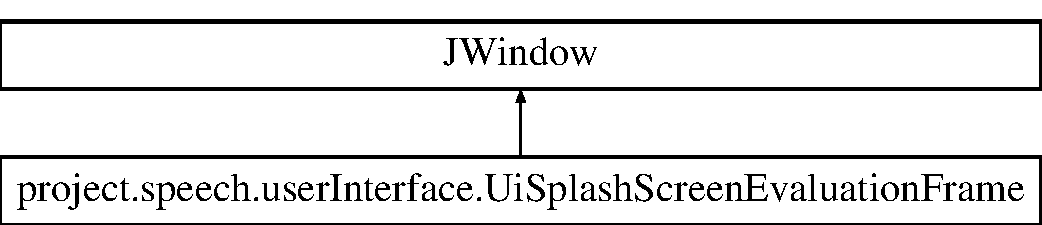
\includegraphics[height=2.000000cm]{classproject_1_1speech_1_1user_interface_1_1_ui_splash_screen_evaluation_frame}
\end{center}
\end{figure}
\subsection*{Public Member Functions}
\begin{DoxyCompactItemize}
\item 
{\bf Ui\+Splash\+Screen\+Evaluation\+Frame} (final File speech\+Database\+Directory, final Array\+List$<$ {\bf Ui\+Asr\+Properties} $>$ asr\+Properties\+Obj, final Array\+List$<$ String $>$ selected\+Performance\+List, final Array\+List$<$ String $>$ selected\+Asr\+List, final String algorithm\+Selected)  throws Invocation\+Target\+Exception, Interrupted\+Exception  
\end{DoxyCompactItemize}
\subsection*{Private Member Functions}
\begin{DoxyCompactItemize}
\item 
J\+Window {\bf create\+G\+U\+I} ()
\end{DoxyCompactItemize}


\subsection{Constructor \& Destructor Documentation}
\index{project\+::speech\+::user\+Interface\+::\+Ui\+Splash\+Screen\+Evaluation\+Frame@{project\+::speech\+::user\+Interface\+::\+Ui\+Splash\+Screen\+Evaluation\+Frame}!Ui\+Splash\+Screen\+Evaluation\+Frame@{Ui\+Splash\+Screen\+Evaluation\+Frame}}
\index{Ui\+Splash\+Screen\+Evaluation\+Frame@{Ui\+Splash\+Screen\+Evaluation\+Frame}!project\+::speech\+::user\+Interface\+::\+Ui\+Splash\+Screen\+Evaluation\+Frame@{project\+::speech\+::user\+Interface\+::\+Ui\+Splash\+Screen\+Evaluation\+Frame}}
\subsubsection[{Ui\+Splash\+Screen\+Evaluation\+Frame}]{\setlength{\rightskip}{0pt plus 5cm}project.\+speech.\+user\+Interface.\+Ui\+Splash\+Screen\+Evaluation\+Frame.\+Ui\+Splash\+Screen\+Evaluation\+Frame (
\begin{DoxyParamCaption}
\item[{final File}]{speech\+Database\+Directory, }
\item[{final Array\+List$<$ {\bf Ui\+Asr\+Properties} $>$}]{asr\+Properties\+Obj, }
\item[{final Array\+List$<$ String $>$}]{selected\+Performance\+List, }
\item[{final Array\+List$<$ String $>$}]{selected\+Asr\+List, }
\item[{final String}]{algorithm\+Selected}
\end{DoxyParamCaption}
) throws Invocation\+Target\+Exception, Interrupted\+Exception}\label{classproject_1_1speech_1_1user_interface_1_1_ui_splash_screen_evaluation_frame_a7e625a2b9162f98b64474ab105a2dd70}


\subsection{Member Function Documentation}
\index{project\+::speech\+::user\+Interface\+::\+Ui\+Splash\+Screen\+Evaluation\+Frame@{project\+::speech\+::user\+Interface\+::\+Ui\+Splash\+Screen\+Evaluation\+Frame}!create\+G\+U\+I@{create\+G\+U\+I}}
\index{create\+G\+U\+I@{create\+G\+U\+I}!project\+::speech\+::user\+Interface\+::\+Ui\+Splash\+Screen\+Evaluation\+Frame@{project\+::speech\+::user\+Interface\+::\+Ui\+Splash\+Screen\+Evaluation\+Frame}}
\subsubsection[{create\+G\+U\+I}]{\setlength{\rightskip}{0pt plus 5cm}J\+Window project.\+speech.\+user\+Interface.\+Ui\+Splash\+Screen\+Evaluation\+Frame.\+create\+G\+U\+I (
\begin{DoxyParamCaption}
{}
\end{DoxyParamCaption}
)\hspace{0.3cm}{\ttfamily [private]}}\label{classproject_1_1speech_1_1user_interface_1_1_ui_splash_screen_evaluation_frame_a584004b3197b1c43b464c669f178bf44}


The documentation for this class was generated from the following file\+:\begin{DoxyCompactItemize}
\item 
project/speech/user\+Interface/{\bf Ui\+Splash\+Screen\+Evaluation\+Frame.\+java}\end{DoxyCompactItemize}

\section{project.\+speech.\+user\+Interface.\+Ui\+Splash\+Screen\+Loading\+Frame Class Reference}
\label{classproject_1_1speech_1_1user_interface_1_1_ui_splash_screen_loading_frame}\index{project.\+speech.\+user\+Interface.\+Ui\+Splash\+Screen\+Loading\+Frame@{project.\+speech.\+user\+Interface.\+Ui\+Splash\+Screen\+Loading\+Frame}}
Inheritance diagram for project.\+speech.\+user\+Interface.\+Ui\+Splash\+Screen\+Loading\+Frame\+:\begin{figure}[H]
\begin{center}
\leavevmode
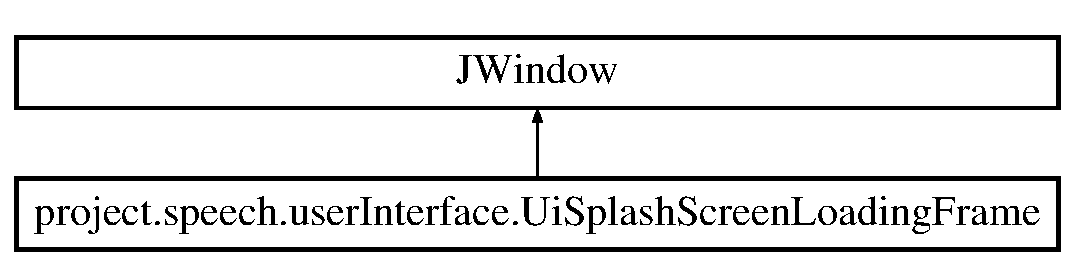
\includegraphics[height=2.000000cm]{classproject_1_1speech_1_1user_interface_1_1_ui_splash_screen_loading_frame}
\end{center}
\end{figure}
\subsection*{Public Member Functions}
\begin{DoxyCompactItemize}
\item 
{\bf Ui\+Splash\+Screen\+Loading\+Frame} ()
\item 
void {\bf show\+Splash} ()
\end{DoxyCompactItemize}
\subsection*{Private Attributes}
\begin{DoxyCompactItemize}
\item 
int {\bf thread\+Count} = 50
\end{DoxyCompactItemize}


\subsection{Constructor \& Destructor Documentation}
\index{project\+::speech\+::user\+Interface\+::\+Ui\+Splash\+Screen\+Loading\+Frame@{project\+::speech\+::user\+Interface\+::\+Ui\+Splash\+Screen\+Loading\+Frame}!Ui\+Splash\+Screen\+Loading\+Frame@{Ui\+Splash\+Screen\+Loading\+Frame}}
\index{Ui\+Splash\+Screen\+Loading\+Frame@{Ui\+Splash\+Screen\+Loading\+Frame}!project\+::speech\+::user\+Interface\+::\+Ui\+Splash\+Screen\+Loading\+Frame@{project\+::speech\+::user\+Interface\+::\+Ui\+Splash\+Screen\+Loading\+Frame}}
\subsubsection[{Ui\+Splash\+Screen\+Loading\+Frame}]{\setlength{\rightskip}{0pt plus 5cm}project.\+speech.\+user\+Interface.\+Ui\+Splash\+Screen\+Loading\+Frame.\+Ui\+Splash\+Screen\+Loading\+Frame (
\begin{DoxyParamCaption}
{}
\end{DoxyParamCaption}
)}\label{classproject_1_1speech_1_1user_interface_1_1_ui_splash_screen_loading_frame_a67469d073d3547a89c5cdff35dff85cf}


\subsection{Member Function Documentation}
\index{project\+::speech\+::user\+Interface\+::\+Ui\+Splash\+Screen\+Loading\+Frame@{project\+::speech\+::user\+Interface\+::\+Ui\+Splash\+Screen\+Loading\+Frame}!show\+Splash@{show\+Splash}}
\index{show\+Splash@{show\+Splash}!project\+::speech\+::user\+Interface\+::\+Ui\+Splash\+Screen\+Loading\+Frame@{project\+::speech\+::user\+Interface\+::\+Ui\+Splash\+Screen\+Loading\+Frame}}
\subsubsection[{show\+Splash}]{\setlength{\rightskip}{0pt plus 5cm}void project.\+speech.\+user\+Interface.\+Ui\+Splash\+Screen\+Loading\+Frame.\+show\+Splash (
\begin{DoxyParamCaption}
{}
\end{DoxyParamCaption}
)}\label{classproject_1_1speech_1_1user_interface_1_1_ui_splash_screen_loading_frame_a1dc347823bf269bb0a78afe1e1f4e8b4}


\subsection{Member Data Documentation}
\index{project\+::speech\+::user\+Interface\+::\+Ui\+Splash\+Screen\+Loading\+Frame@{project\+::speech\+::user\+Interface\+::\+Ui\+Splash\+Screen\+Loading\+Frame}!thread\+Count@{thread\+Count}}
\index{thread\+Count@{thread\+Count}!project\+::speech\+::user\+Interface\+::\+Ui\+Splash\+Screen\+Loading\+Frame@{project\+::speech\+::user\+Interface\+::\+Ui\+Splash\+Screen\+Loading\+Frame}}
\subsubsection[{thread\+Count}]{\setlength{\rightskip}{0pt plus 5cm}int project.\+speech.\+user\+Interface.\+Ui\+Splash\+Screen\+Loading\+Frame.\+thread\+Count = 50\hspace{0.3cm}{\ttfamily [private]}}\label{classproject_1_1speech_1_1user_interface_1_1_ui_splash_screen_loading_frame_a341c1250f1395e233d57291cbfcbbc0b}


The documentation for this class was generated from the following file\+:\begin{DoxyCompactItemize}
\item 
project/speech/user\+Interface/{\bf Ui\+Splash\+Screen\+Loading\+Frame.\+java}\end{DoxyCompactItemize}

\chapter{File Documentation}
\section{project/speech/asrengines/\+Cmu\+Sphinx\+Engine.java File Reference}
\label{_cmu_sphinx_engine_8java}\index{project/speech/asrengines/\+Cmu\+Sphinx\+Engine.\+java@{project/speech/asrengines/\+Cmu\+Sphinx\+Engine.\+java}}
\subsection*{Classes}
\begin{DoxyCompactItemize}
\item 
class {\bf project.\+speech.\+asrengines.\+Cmu\+Sphinx\+Engine}
\end{DoxyCompactItemize}
\subsection*{Packages}
\begin{DoxyCompactItemize}
\item 
package {\bf project.\+speech.\+asrengines}
\end{DoxyCompactItemize}

\section{project/speech/asrengines/\+Ispeech\+Engine.java File Reference}
\label{_ispeech_engine_8java}\index{project/speech/asrengines/\+Ispeech\+Engine.\+java@{project/speech/asrengines/\+Ispeech\+Engine.\+java}}
\subsection*{Classes}
\begin{DoxyCompactItemize}
\item 
class {\bf project.\+speech.\+asrengines.\+Ispeech\+Engine}
\end{DoxyCompactItemize}
\subsection*{Packages}
\begin{DoxyCompactItemize}
\item 
package {\bf project.\+speech.\+asrengines}
\end{DoxyCompactItemize}

\section{project/speech/evaluationsystem/\+Evaluation\+System.java File Reference}
\label{_evaluation_system_8java}\index{project/speech/evaluationsystem/\+Evaluation\+System.\+java@{project/speech/evaluationsystem/\+Evaluation\+System.\+java}}
\subsection*{Classes}
\begin{DoxyCompactItemize}
\item 
class {\bf project.\+speech.\+evaluationsystem.\+Evaluation\+System}
\end{DoxyCompactItemize}
\subsection*{Packages}
\begin{DoxyCompactItemize}
\item 
package {\bf project.\+speech.\+evaluationsystem}
\end{DoxyCompactItemize}

\section{project/speech/evaluator/\+Evaluation\+Aligner.java File Reference}
\label{_evaluation_aligner_8java}\index{project/speech/evaluator/\+Evaluation\+Aligner.\+java@{project/speech/evaluator/\+Evaluation\+Aligner.\+java}}
\subsection*{Classes}
\begin{DoxyCompactItemize}
\item 
class {\bf project.\+speech.\+evaluator.\+Evaluation\+Aligner}
\end{DoxyCompactItemize}
\subsection*{Packages}
\begin{DoxyCompactItemize}
\item 
package {\bf project.\+speech.\+evaluator}
\end{DoxyCompactItemize}

\section{project/speech/evaluator/\+Evaluator\+Result.java File Reference}
\label{_evaluator_result_8java}\index{project/speech/evaluator/\+Evaluator\+Result.\+java@{project/speech/evaluator/\+Evaluator\+Result.\+java}}
\subsection*{Classes}
\begin{DoxyCompactItemize}
\item 
class {\bf project.\+speech.\+evaluator.\+Evaluator\+Result}
\end{DoxyCompactItemize}
\subsection*{Packages}
\begin{DoxyCompactItemize}
\item 
package {\bf project.\+speech.\+evaluator}
\end{DoxyCompactItemize}

\section{project/speech/global\+Access/\+Globals.java File Reference}
\label{_globals_8java}\index{project/speech/global\+Access/\+Globals.\+java@{project/speech/global\+Access/\+Globals.\+java}}
\subsection*{Classes}
\begin{DoxyCompactItemize}
\item 
class {\bf project.\+speech.\+global\+Access.\+Globals}
\end{DoxyCompactItemize}
\subsection*{Packages}
\begin{DoxyCompactItemize}
\item 
package {\bf project.\+speech.\+global\+Access}
\end{DoxyCompactItemize}

\section{project/speech/reader\+And\+Writer/\+File\+Details.java File Reference}
\label{_file_details_8java}\index{project/speech/reader\+And\+Writer/\+File\+Details.\+java@{project/speech/reader\+And\+Writer/\+File\+Details.\+java}}
\subsection*{Classes}
\begin{DoxyCompactItemize}
\item 
class {\bf project.\+speech.\+reader\+And\+Writer.\+File\+Details}
\end{DoxyCompactItemize}
\subsection*{Packages}
\begin{DoxyCompactItemize}
\item 
package {\bf project.\+speech.\+reader\+And\+Writer}
\end{DoxyCompactItemize}

\section{project/speech/reader\+And\+Writer/\+File\+Reader.java File Reference}
\label{_file_reader_8java}\index{project/speech/reader\+And\+Writer/\+File\+Reader.\+java@{project/speech/reader\+And\+Writer/\+File\+Reader.\+java}}
\subsection*{Classes}
\begin{DoxyCompactItemize}
\item 
class {\bf project.\+speech.\+reader\+And\+Writer.\+File\+Reader}
\end{DoxyCompactItemize}
\subsection*{Packages}
\begin{DoxyCompactItemize}
\item 
package {\bf project.\+speech.\+reader\+And\+Writer}
\end{DoxyCompactItemize}

\section{project/speech/reader\+And\+Writer/\+File\+Scripter.java File Reference}
\label{_file_scripter_8java}\index{project/speech/reader\+And\+Writer/\+File\+Scripter.\+java@{project/speech/reader\+And\+Writer/\+File\+Scripter.\+java}}
\subsection*{Classes}
\begin{DoxyCompactItemize}
\item 
class {\bf project.\+speech.\+reader\+And\+Writer.\+File\+Scripter}
\end{DoxyCompactItemize}
\subsection*{Packages}
\begin{DoxyCompactItemize}
\item 
package {\bf project.\+speech.\+reader\+And\+Writer}
\end{DoxyCompactItemize}

\section{project/speech/user\+Interface/\+Ui\+Asr\+Properties.java File Reference}
\label{_ui_asr_properties_8java}\index{project/speech/user\+Interface/\+Ui\+Asr\+Properties.\+java@{project/speech/user\+Interface/\+Ui\+Asr\+Properties.\+java}}
\subsection*{Classes}
\begin{DoxyCompactItemize}
\item 
class {\bf project.\+speech.\+user\+Interface.\+Ui\+Asr\+Properties}
\end{DoxyCompactItemize}
\subsection*{Packages}
\begin{DoxyCompactItemize}
\item 
package {\bf project.\+speech.\+user\+Interface}
\end{DoxyCompactItemize}

\section{project/speech/user\+Interface/\+Ui\+Instruction\+Frame1.java File Reference}
\label{_ui_instruction_frame1_8java}\index{project/speech/user\+Interface/\+Ui\+Instruction\+Frame1.\+java@{project/speech/user\+Interface/\+Ui\+Instruction\+Frame1.\+java}}
\subsection*{Classes}
\begin{DoxyCompactItemize}
\item 
class {\bf project.\+speech.\+user\+Interface.\+Ui\+Instruction\+Frame1}
\end{DoxyCompactItemize}
\subsection*{Packages}
\begin{DoxyCompactItemize}
\item 
package {\bf project.\+speech.\+user\+Interface}
\end{DoxyCompactItemize}

\section{project/speech/user\+Interface/\+Ui\+Instruction\+Frame2.java File Reference}
\label{_ui_instruction_frame2_8java}\index{project/speech/user\+Interface/\+Ui\+Instruction\+Frame2.\+java@{project/speech/user\+Interface/\+Ui\+Instruction\+Frame2.\+java}}
\subsection*{Classes}
\begin{DoxyCompactItemize}
\item 
class {\bf project.\+speech.\+user\+Interface.\+Ui\+Instruction\+Frame2}
\end{DoxyCompactItemize}
\subsection*{Packages}
\begin{DoxyCompactItemize}
\item 
package {\bf project.\+speech.\+user\+Interface}
\end{DoxyCompactItemize}

\section{project/speech/user\+Interface/\+Ui\+Instruction\+Main\+Frame.java File Reference}
\label{_ui_instruction_main_frame_8java}\index{project/speech/user\+Interface/\+Ui\+Instruction\+Main\+Frame.\+java@{project/speech/user\+Interface/\+Ui\+Instruction\+Main\+Frame.\+java}}
\subsection*{Classes}
\begin{DoxyCompactItemize}
\item 
class {\bf project.\+speech.\+user\+Interface.\+Ui\+Instruction\+Main\+Frame}
\end{DoxyCompactItemize}
\subsection*{Packages}
\begin{DoxyCompactItemize}
\item 
package {\bf project.\+speech.\+user\+Interface}
\end{DoxyCompactItemize}

\section{project/speech/user\+Interface/\+Ui\+Main\+Frame.java File Reference}
\label{_ui_main_frame_8java}\index{project/speech/user\+Interface/\+Ui\+Main\+Frame.\+java@{project/speech/user\+Interface/\+Ui\+Main\+Frame.\+java}}
\subsection*{Classes}
\begin{DoxyCompactItemize}
\item 
class {\bf project.\+speech.\+user\+Interface.\+Ui\+Main\+Frame}
\end{DoxyCompactItemize}
\subsection*{Packages}
\begin{DoxyCompactItemize}
\item 
package {\bf project.\+speech.\+user\+Interface}
\end{DoxyCompactItemize}

\section{project/speech/user\+Interface/\+Ui\+Method1\+Frame.java File Reference}
\label{_ui_method1_frame_8java}\index{project/speech/user\+Interface/\+Ui\+Method1\+Frame.\+java@{project/speech/user\+Interface/\+Ui\+Method1\+Frame.\+java}}
\subsection*{Classes}
\begin{DoxyCompactItemize}
\item 
class {\bf project.\+speech.\+user\+Interface.\+Ui\+Method1\+Frame}
\end{DoxyCompactItemize}
\subsection*{Packages}
\begin{DoxyCompactItemize}
\item 
package {\bf project.\+speech.\+user\+Interface}
\end{DoxyCompactItemize}

\section{project/speech/user\+Interface/\+Ui\+Method2\+Frame.java File Reference}
\label{_ui_method2_frame_8java}\index{project/speech/user\+Interface/\+Ui\+Method2\+Frame.\+java@{project/speech/user\+Interface/\+Ui\+Method2\+Frame.\+java}}
\subsection*{Classes}
\begin{DoxyCompactItemize}
\item 
class {\bf project.\+speech.\+user\+Interface.\+Ui\+Method2\+Frame}
\end{DoxyCompactItemize}
\subsection*{Packages}
\begin{DoxyCompactItemize}
\item 
package {\bf project.\+speech.\+user\+Interface}
\end{DoxyCompactItemize}

\section{project/speech/user\+Interface/\+Ui\+Result\+Frame1.java File Reference}
\label{_ui_result_frame1_8java}\index{project/speech/user\+Interface/\+Ui\+Result\+Frame1.\+java@{project/speech/user\+Interface/\+Ui\+Result\+Frame1.\+java}}
\subsection*{Classes}
\begin{DoxyCompactItemize}
\item 
class {\bf project.\+speech.\+user\+Interface.\+Ui\+Result\+Frame1}
\end{DoxyCompactItemize}
\subsection*{Packages}
\begin{DoxyCompactItemize}
\item 
package {\bf project.\+speech.\+user\+Interface}
\end{DoxyCompactItemize}

\section{project/speech/user\+Interface/\+Ui\+Splash\+Screen\+Evaluation\+Frame.java File Reference}
\label{_ui_splash_screen_evaluation_frame_8java}\index{project/speech/user\+Interface/\+Ui\+Splash\+Screen\+Evaluation\+Frame.\+java@{project/speech/user\+Interface/\+Ui\+Splash\+Screen\+Evaluation\+Frame.\+java}}
\subsection*{Classes}
\begin{DoxyCompactItemize}
\item 
class {\bf project.\+speech.\+user\+Interface.\+Ui\+Splash\+Screen\+Evaluation\+Frame}
\item 
class {\bfseries project.\+speech.\+user\+Interface.\+My\+Swing\+Worker}
\end{DoxyCompactItemize}
\subsection*{Packages}
\begin{DoxyCompactItemize}
\item 
package {\bf project.\+speech.\+user\+Interface}
\end{DoxyCompactItemize}

\section{project/speech/user\+Interface/\+Ui\+Splash\+Screen\+Loading\+Frame.java File Reference}
\label{_ui_splash_screen_loading_frame_8java}\index{project/speech/user\+Interface/\+Ui\+Splash\+Screen\+Loading\+Frame.\+java@{project/speech/user\+Interface/\+Ui\+Splash\+Screen\+Loading\+Frame.\+java}}
\subsection*{Classes}
\begin{DoxyCompactItemize}
\item 
class {\bf project.\+speech.\+user\+Interface.\+Ui\+Splash\+Screen\+Loading\+Frame}
\end{DoxyCompactItemize}
\subsection*{Packages}
\begin{DoxyCompactItemize}
\item 
package {\bf project.\+speech.\+user\+Interface}
\end{DoxyCompactItemize}

%--- End generated contents ---

% Index
\backmatter
\newpage
\phantomsection
\clearemptydoublepage
\addcontentsline{toc}{chapter}{Index}
\printindex

\end{document}
